\documentclass[11pt]{article}
% ======================================================================
% Shared preamble for the InfoVis study guide.
% Section files may rely ONLY on the packages, environments and macros
% defined here. Do NOT \usepackage anything else inside section files.
% ======================================================================
\usepackage[utf8]{inputenc}
\usepackage[T1]{fontenc}
\usepackage{lmodern}
\usepackage[a4paper,margin=2.3cm]{geometry}
\usepackage{microtype}
\usepackage{amsmath,amssymb}
\usepackage{booktabs}
\usepackage{array}
\usepackage{longtable}
\usepackage{enumitem}
\usepackage{xcolor}
\usepackage{graphicx}
\usepackage{tikz}
\usetikzlibrary{arrows.meta,positioning,shapes.geometric,fit,calc}
\usepackage[most]{tcolorbox}
\usepackage{hyperref}
\hypersetup{colorlinks=true,linkcolor=tuwblue,urlcolor=tuwblue,citecolor=tuwblue,
  pdftitle={Information Visualization -- Exam Study Guide}}
\usepackage{titlesec}

% --- Colours -----------------------------------------------------------
\definecolor{tuwblue}{RGB}{0,102,153}
\definecolor{tuwdark}{RGB}{0,72,110}
\definecolor{boxgray}{RGB}{245,246,248}
\definecolor{keygreen}{RGB}{0,120,80}
\definecolor{pitred}{RGB}{170,40,40}
\definecolor{examorange}{RGB}{200,110,0}
\definecolor{rulec}{RGB}{210,214,220}

% --- Section styling ---------------------------------------------------
\titleformat{\section}{\Large\bfseries\color{tuwdark}}{\thesection}{0.6em}{}
\titleformat{\subsection}{\large\bfseries\color{tuwblue}}{\thesubsection}{0.6em}{}
\titleformat{\subsubsection}{\normalsize\bfseries\color{tuwblue}}{\thesubsubsection}{0.6em}{}
\setlist{topsep=2pt,itemsep=1pt,parsep=0pt}

% --- Reusable boxes ----------------------------------------------------
% Key points / definitions
\newtcolorbox{keybox}[1][Key points]{
  enhanced, breakable, colback=boxgray, colframe=tuwblue,
  coltitle=white, fonttitle=\bfseries, title={#1},
  boxrule=0.6pt, arc=2pt, left=4pt,right=4pt,top=3pt,bottom=3pt}

% Algorithm fact-sheet
\newtcolorbox{algobox}[1][Algorithm]{
  enhanced, breakable, colback=white, colframe=tuwdark,
  coltitle=white, fonttitle=\bfseries, title={#1},
  boxrule=0.7pt, arc=2pt, left=4pt,right=4pt,top=3pt,bottom=3pt}

% Exam tip / how this is asked
\newtcolorbox{exambox}[1][Exam angle]{
  enhanced, breakable, colback=examorange!8, colframe=examorange,
  coltitle=white, fonttitle=\bfseries, title={#1},
  boxrule=0.6pt, arc=2pt, left=4pt,right=4pt,top=3pt,bottom=3pt}

% Common pitfall / point deduction
\newtcolorbox{pitfall}[1][Pitfall / point deduction]{
  enhanced, breakable, colback=pitred!7, colframe=pitred,
  coltitle=white, fonttitle=\bfseries, title={#1},
  boxrule=0.6pt, arc=2pt, left=4pt,right=4pt,top=3pt,bottom=3pt}

% Worked / practice question
\newtcolorbox{qbox}[1][Practice question]{
  enhanced, breakable, colback=keygreen!6, colframe=keygreen,
  coltitle=white, fonttitle=\bfseries, title={#1},
  boxrule=0.6pt, arc=2pt, left=4pt,right=4pt,top=3pt,bottom=3pt}

% Inline helper for "sketch this" descriptions
\newcommand{\sketchnote}[1]{\par\smallskip\noindent\textit{\textcolor{tuwblue}{Sketch:}} #1\par\smallskip}
% Term emphasis
\newcommand{\term}[1]{\textbf{#1}}


\title{\vspace{-1.2cm}\textbf{\textcolor{tuwdark}{Information Visualization}}\\[2mm]
       \Large\textcolor{tuwblue}{Comprehensive Exam Study Guide}\\[2mm]
       \normalsize TU Wien, 2026S\,\textemdash\,based on the lecture slides and mandatory readings}
\author{}
\date{}

\begin{document}
\maketitle
\vspace{-1.4cm}
\begin{center}\small\itshape
This guide is organised by content domain (Sections 1--12) followed by an
exam playbook, an algorithm cheat-sheet, list-style quick references and
practice questions (Sections 13--16). Boxes mark \textcolor{tuwblue}{key points},
\textcolor{tuwdark}{algorithm fact-sheets}, \textcolor{examorange}{exam angles}
and \textcolor{pitred}{common point deductions}.
\end{center}
\vspace{2mm}
\hrule
\tableofcontents
\clearpage

\section{Foundations of Information Visualization}

\subsection{What is Information Visualization?}

The standard definition used in the lecture is from Card, Mackinlay \& Shneiderman:

\begin{keybox}[Definition]
\term{Information Visualization} is ``the use of \emph{computer-supported},
\emph{interactive}, \emph{visual} representations of \emph{abstract data} to
\emph{amplify cognition}.'' \hfill \textit{[Card et al., 1999]}
\end{keybox}

Each highlighted word is load-bearing:
\begin{itemize}
  \item \term{computer-supported} -- the visualization is generated and (re-)rendered by a computer, not drawn once by hand.
  \item \term{interactive} -- the user can manipulate the view (filter, zoom, select, re-map). Interactivity is what distinguishes InfoVis from a static print figure.
  \item \term{visual representation} -- data is encoded into visual marks and channels so the human visual system can read it.
  \item \term{abstract data} -- the data has \emph{no inherent spatial mapping} (tables, networks, text), in contrast to scientific visualization where space is given (medical scans, flow fields).
  \item \term{amplify cognition} -- the purpose. \emph{Cognition} = ``the mental process of acquiring knowledge and understanding through thought, experience, and the senses'' [Oxford]. A later Card quote sharpens the point: ``The purpose of information visualization is to amplify cognitive performance, \emph{not just to create interesting pictures.}''
\end{itemize}

\subsubsection{What -- Why -- How}
The lecture frames the whole field with three questions (this maps directly onto Munzner's framework, see below):
\begin{itemize}
  \item \term{What?} Abstract data.
  \item \term{Why?} To amplify cognition.
  \item \term{How?} Visual representations + interactivity.
\end{itemize}
Mechanistically, visualization \term{expands human working memory}: instead of holding facts in the head, the user offloads them onto an external display (\term{external cognition}). The design challenge is to find the \term{most expressive and effective} visualization, turning insights into knowledge.

\subsection{High-Level Goals: Exploration, Confirmation, Presentation}

Visualization serves three high-level goals, ordered here by how much \term{interactivity} they typically need (most $\rightarrow$ least):

\begin{center}
\begin{tabular}{@{}lll@{}}
\toprule
\textbf{Goal} & \textbf{Description} & \textbf{Interactivity} \\
\midrule
\term{Exploration}  & Searching / analysing data \emph{without} a prior & high \\
                    & hypothesis, to find potentially useful info & \\
\term{Confirmation} & Goal-oriented examination of \emph{hypotheses} & medium \\
\term{Presentation} & Efficiently \& effectively \emph{communicate} facts & low \\
\bottomrule
\end{tabular}
\end{center}

\begin{center}
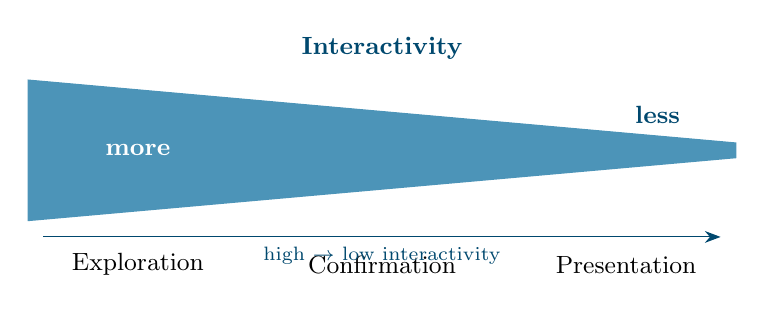
\begin{tikzpicture}[font=\small]
  % wedge: thick on the left, thin on the right
  \fill[tuwblue!70] (0,-0.9) -- (0,0.9) -- (9,0.1) -- (9,-0.1) -- cycle;
  \node[white] at (1.4,0) {\bfseries more};
  \node[tuwdark] at (8.0,0.45) {\bfseries less};
  \node[tuwdark] at (4.5,1.3) {\bfseries Interactivity};
  % goal labels underneath, aligned to wedge regions
  \node[align=center] at (1.4,-1.45) {Exploration};
  \node[align=center] at (4.5,-1.45) {Confirmation};
  \node[align=center] at (7.6,-1.45) {Presentation};
  \draw[-{Stealth[length=2mm]}, tuwdark] (0.2,-1.1) -- (8.8,-1.1)
    node[midway, below, font=\scriptsize] {high $\rightarrow$ low interactivity};
\end{tikzpicture}
\end{center}
\sketchnote{Draw a horizontal triangle/wedge for ``interactivity'' that is thick on the left (Exploration) and thin on the right (Presentation); label the three goals underneath.}

Exploration is the open-ended, \emph{exploratory} mode; confirmation and presentation are the \emph{explanatory / confirmatory} modes. A dashboard (e.g.\ Tableau) is exploratory; John Snow's 1854 cholera map is confirmatory/presentational; a New York Times infographic is presentational.

\begin{keybox}[Why we still need visualization -- Anscombe / Datasaurus]
\term{Anscombe's Quartet} (and the \term{Datasaurus Dozen}) are four/twelve datasets with \emph{identical summary statistics} -- same mean ($\bar x{=}9,\bar y{=}7.5$), same variance ($s_x^2{=}11,s_y^2{=}4.12$), same correlation, same linear regression ($y=0.5x+3$) -- yet \emph{completely different shapes} when plotted. Summary statistics (and an LLM that only reads the numbers) can be badly misled; only the visualization reveals curvature, outliers, and clustering.
\end{keybox}

\subsection{The InfoVis Reference Model (Pipeline)}

The lecture's ``How to visualize?'' answer is the classic \term{InfoVis reference model} (Card / Mackinlay): a pipeline of four data states connected by three transforms, all steerable by the user.

\begin{center}
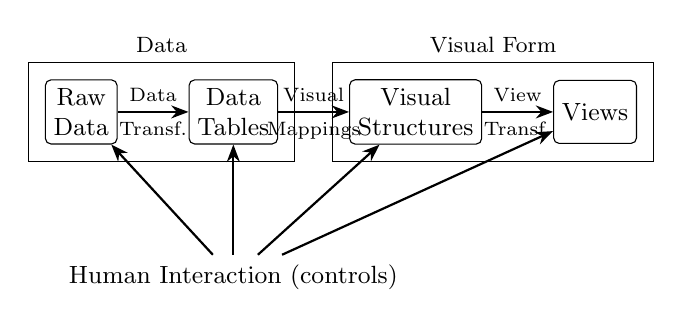
\begin{tikzpicture}[
  node distance=8mm and 9mm,
  box/.style={draw, rounded corners=2pt, align=center, minimum height=8mm, inner sep=3pt, font=\small},
  arr/.style={-{Stealth[length=2.2mm]}, thick}]
  \node[box] (raw)  {Raw\\Data};
  \node[box, right=of raw]  (tab)  {Data\\Tables};
  \node[box, right=of tab]  (vis)  {Visual\\Structures};
  \node[box, right=of vis]  (view) {Views};
  \draw[arr] (raw)  -- node[above,font=\scriptsize]{Data}     node[below,font=\scriptsize]{Transf.} (tab);
  \draw[arr] (tab)  -- node[above,font=\scriptsize]{Visual}   node[below,font=\scriptsize]{Mappings} (vis);
  \draw[arr] (vis)  -- node[above,font=\scriptsize]{View}     node[below,font=\scriptsize]{Transf.} (view);
  \node[draw, fit=(raw)(tab), inner sep=6pt, label=above:\footnotesize Data] {};
  \node[draw, fit=(vis)(view), inner sep=6pt, label=above:\footnotesize Visual Form] {};
  \node[below=14mm of tab, font=\small] (h) {Human Interaction (controls)};
  \draw[arr] (h) -- (raw);
  \draw[arr] (h) -- (tab);
  \draw[arr] (h) -- (vis);
  \draw[arr] (h) -- (view);
\end{tikzpicture}
\end{center}

\begin{itemize}
  \item \term{Raw Data} $\xrightarrow{\text{Data Transformations}}$ \term{Data Tables} -- clean, derive, restructure (the ``Data'' stage; covered in Section~2).
  \item \term{Data Tables} $\xrightarrow{\text{Visual Mappings}}$ \term{Visual Structures} -- assign spatial substrate, marks and visual channels (the key step; ``Visual Form'').
  \item \term{Visual Structures} $\xrightarrow{\text{View Transformations}}$ \term{Views} -- navigation, zoom, distortion, selection.
  \item \term{Human Interaction (controls)} feeds back into \emph{every} transform, and the whole loop is driven by the user's \term{Task}.
\end{itemize}

\begin{pitfall}[Common pitfall]
Do not collapse the pipeline. The three transforms are distinct: \emph{data transformation} ($\neq$ visual mapping) happens \emph{before} anything visual exists; \emph{visual mapping} is data~$\rightarrow$~marks/channels; \emph{view transformation} is on the already-rendered structure. Forgetting that interaction feeds back into all stages also loses points.
\end{pitfall}

\subsection{Munzner's What--Why--How Analysis Framework}

The mandatory reading (Munzner, 2014) structures any visualization design/analysis around three \term{nested} questions:

\begin{keybox}[The three nested questions]
\begin{itemize}
  \item \term{What?} -- the \term{data abstraction}: which dataset and attribute types are involved (Section~2).
  \item \term{Why?} -- the \term{task abstraction}: what the user wants to accomplish (e.g.\ discover, present, compare, locate trends/outliers).
  \item \term{How?} -- the \term{idiom}: \term{visual encoding} (marks + channels) and \term{interaction design} that solve the what/why.
\end{itemize}
\end{keybox}

\emph{Nested} means the answers are dependent: the \emph{how} you choose must fit the \emph{what} and the \emph{why}. A core skill (heavily tested) is to translate a \emph{domain-specific} problem into this \emph{abstract} vocabulary so that solutions transfer across domains. Example: ``age, BMI, glucose, eGFR for some patients'' and ``vehicles, accidents, deaths, population per Austrian state'' are, abstractly, the \emph{same} thing -- a table of items with one categorical key and several quantitative attributes.

\subsection{Human-in-the-Loop vs Pure Automation}

\begin{keybox}[When to visualize, when to automate]
\begin{itemize}
  \item \term{Pure automatic methods} work \emph{only for clearly specified problems} (a well-defined question, a known model).
  \item \term{Pure visualization} is \emph{not enough} for very large and complex data.
  \item Use \term{visualization / a human in the loop} when the problem is \emph{ill-specified}, exploratory, or requires judgement, and when you need to leverage the human visual system to spot the unexpected.
\end{itemize}
\end{keybox}

This is the rationale for \term{Visual Analytics}: a feedback loop coupling automated data analysis (data mining, model building) with interactive visualization, so that \term{visual data exploration} (Data $\rightarrow$ Visualization $\rightarrow$ Knowledge, with user interaction and parameter refinement) and automated analysis reinforce each other. Classic example: an \term{outlier} that a regression line would average over is spotted visually, inspected with external context, and removed by the analyst.

\begin{exambox}[How this is asked]
Typical exam tasks for this section: \emph{(1)} state and explain the Card definition word by word; \emph{(2)} name and order the three high-level goals and link them to interactivity; \emph{(3)} draw / label the InfoVis reference model and name the three transforms; \emph{(4)} give Munzner's three nested questions and explain why they are nested; \emph{(5)} argue when visualization beats pure automation, often via Anscombe's Quartet. Expect ``define X'' and ``draw the pipeline'' phrasing.
\end{exambox}

\subsection{Resource Limitations}

A good design respects three limited resources (Munzner). Trade-offs between them drive most design decisions.

\begin{center}
\begin{tabular}{@{}ll@{}}
\toprule
\textbf{Resource} & \textbf{Limit / consequence} \\
\midrule
\term{Computer}  & computation time and memory; large data $\rightarrow$ slow or infeasible idioms \\
\term{Human}     & attention, working memory, perceptual/cognitive capacity \\
\term{Display}   & finite pixels (screen real estate); the information-density vs clutter trade-off \\
\bottomrule
\end{tabular}
\end{center}

\subsection{Visualization Disciplines and the Design Triangle}

\begin{itemize}
  \item \term{Information Visualization (InfoVis)} -- spatial layout is \emph{chosen} by the designer (abstract data).
  \item \term{Scientific Visualization (SciVis)} -- spatial position is \emph{given} with the data (continuous fields, e.g.\ medical scans).
  \item \term{Visual Analytics / Visual Data Science} -- visualization $+$ automated analysis in a human-in-the-loop.
\end{itemize}

The \term{design triangle} [Miksch \& Aigner] ties it together: good interactive (visual analytics) methods sit between \term{data}, \term{users} and \term{tasks}, and must be \term{expressive} (w.r.t.\ data), \term{effective} (w.r.t.\ users/perception) and \term{appropriate} (w.r.t.\ tasks).

\begin{pitfall}[Minimalistic design -- chartjunk]
Tufte: ``interior decoration of graphics generates a lot of ink that does not tell the viewer anything new \dots\ it is often \term{chartjunk}.'' Maximise the \term{data-ink ratio} $=\dfrac{\text{data-ink}}{\text{total ink}}$. (Caveat from Bateman et al.\ CHI~2010: embellished ``infographic'' charts had comparable interpretation accuracy and \emph{better long-term recall} -- so chartjunk is not always strictly worse, but for analysis tasks favour minimal designs.)
\end{pitfall}

\section{Data Abstraction}

This section answers Munzner's \term{What?} question: the abstract description of the
data, independent of any domain. The take-away from the lecture is to
\term{describe data in abstract form, not in domain-specific form}; from an
abstract perspective two unrelated domain datasets can be \emph{equivalent}.

\begin{keybox}[The big picture -- one paragraph]
The four basic \term{dataset types} are \term{tables}, \term{networks/trees},
\term{fields}, and \term{geometry}; other groupings of items are
\term{clusters}, \term{sets}, and \term{lists}. They are built from five
\term{data types}: \term{items}, \term{attributes}, \term{links},
\term{positions}, \term{grids}. An attribute's type is \term{categorical} or
\term{ordered}, with ordered split into \term{ordinal} and \term{quantitative};
the ordering direction can be \term{sequential}, \term{diverging}, or
\term{cyclic}. Any dataset can be \term{static} (a file, available all at once)
or \term{dynamic} (a stream).
\end{keybox}

\subsection{Semantics vs Type}

Two crosscutting properties must be known about every value:
\begin{itemize}
  \item \term{Semantics} -- the real-world \emph{meaning} (is this number an age, a postal code, a position?).
  \item \term{Type} -- the structural / mathematical interpretation (item, link, attribute; table, tree, field; what arithmetic is allowed).
\end{itemize}
They are independent: knowing the type does not tell you the semantics. Munzner's
example: the row \texttt{Basil, 7, S, Pear} is meaningless until you are told the
semantics (a person: name, age, shirt size, favourite fruit). Information that
must be supplied alongside the data is \term{metadata}.

\subsection{The Five Data Types}

\begin{center}
\begin{tabular}{@{}lp{8.6cm}@{}}
\toprule
\textbf{Data type} & \textbf{Meaning} \\
\midrule
\term{Item}     & an individual, discrete entity (a row in a table, a node in a network) \\
\term{Attribute}& a property that can be measured, observed or logged (a column); synonyms: \emph{variable}, \emph{dimension} \\
\term{Link}     & a relationship between items, typically within a network; synonym: \emph{edge} \\
\term{Position} & spatial data: a location in 2D or 3D space (e.g.\ a lat--long pair) \\
\term{Grid}     & the strategy for sampling a continuous field (geometric + topological structure of cells) \\
\bottomrule
\end{tabular}
\end{center}

\subsection{The Four Dataset Types (+ Clusters/Sets/Lists)}

\begin{center}
\begin{tabular}{@{}l l p{6.2cm}@{}}
\toprule
\textbf{Dataset type} & \textbf{Built from} & \textbf{Notes} \\
\midrule
\term{Tables}          & items, attributes & flat or multidimensional; cells hold values \\
\term{Networks/Trees}  & items (nodes), links, attributes & \term{tree} = network with hierarchy, no cycles \\
\term{Fields}          & grids, positions, attributes & \emph{continuous}; cells sampled from a continuous domain \\
\term{Geometry}        & items, positions & shape with explicit spatial position; need not have attributes \\
\bottomrule
\end{tabular}
\end{center}

\begin{itemize}
  \item \term{Tables} -- rows = items, columns = attributes; each \term{cell} = (item, attribute) pair holding a \term{value}.
  \item \term{Networks} -- items are \term{nodes} (\emph{vertices}), connected by \term{links} (\emph{edges}); both nodes and links may carry attributes. A \term{tree} is the hierarchical special case (each node has one parent, no cycles).
  \item \term{Fields} -- each \term{cell} contains a measurement from a \term{continuous} domain (infinitely many possible values), requiring \term{sampling} and \term{interpolation}. Tables/networks are \term{discrete} by contrast. A \term{spatial field} samples at spatial positions (e.g.\ a medical scan). By \emph{number of values per cell}: \term{scalar} (1), \term{vector} (2--3, direction+magnitude), \term{tensor} (many). \emph{SciVis} deals with spatial fields (position \emph{given}); \emph{InfoVis} with nonspatial/abstract data (position \emph{chosen}).
  \item \term{Geometry} -- pure shape (points, lines/curves, surfaces, volumes); the odd one out because it need not have attributes.
\end{itemize}

Other groupings of items (not basic dataset types):
\begin{itemize}
  \item \term{Set} -- an \emph{unordered} group of items.
  \item \term{List} -- a group with a \emph{specified ordering} (synonym in CS: \emph{array}).
  \item \term{Cluster} -- a grouping by \emph{attribute similarity} (items in a cluster are more similar to each other than to items in other clusters).
\end{itemize}
More complex structures: a \term{path} (ordered set of segments through a network) and a \term{compound network} (a network plus an associated tree over its nodes). Real datasets are often hybrid combinations.

\subsection{Grid Types (for fields)}
\term{Uniform} (regular intervals; no need to store geometry/topology) $\rightarrow$
\term{rectilinear} (nonuniform spacing) $\rightarrow$ \term{structured} (curvilinear
shapes, store geometry) $\rightarrow$ \term{unstructured} (store both geometry and
topology explicitly).

\subsection{Attribute Types}

\begin{center}
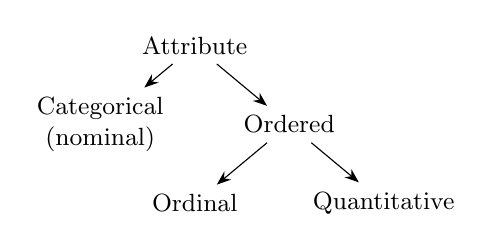
\begin{tikzpicture}[
  every node/.style={font=\small, align=center},
  level distance=10mm, sibling distance=24mm,
  edge from parent/.style={draw,-{Stealth[length=1.8mm]}}]
  \node {Attribute}
    child {node {Categorical\\(nominal)}}
    child {node {Ordered}
      child {node {Ordinal}}
      child {node {Quantitative}}
    };
\end{tikzpicture}
\end{center}

\begin{itemize}
  \item \term{Categorical} (\emph{nominal}) -- \emph{no} implicit ordering; can only tell \emph{same} (apples) vs \emph{different} (apples vs oranges). E.g.\ fruit, genres, file types, city names. Any ordering (alphabetical) is external, not inherent.
  \item \term{Ordered} -- has an implicit ordering. Two sub-types:
  \begin{itemize}
    \item \term{Ordinal} -- well-defined ordering / ranking, but \emph{no full arithmetic}. E.g.\ shirt size: \emph{large $-$ medium} is meaningless, but medium falls between small and large.
    \item \term{Quantitative} -- measurement of magnitude supporting \emph{arithmetic comparison} (e.g.\ $68\text{ in}-42\text{ in}=26\text{ in}$). E.g.\ height, weight, temperature, counts. (Interval vs ratio is usually collapsed.)
  \end{itemize}
\end{itemize}

\subsubsection{Ordering Direction (for ordered attributes)}
\begin{itemize}
  \item \term{Sequential} -- homogeneous range from a minimum to a maximum (e.g.\ mountain height from sea level to peak).
  \item \term{Diverging} -- two sequences meeting at a common \emph{zero/neutral} point (e.g.\ elevation above/below sea level).
  \item \term{Cyclic} -- values wrap around to the start (typically time: hour of day, day of week, month of year).
\end{itemize}

\sketchnote{Sequential = a single arrow $\rightarrow$; diverging = a double-headed arrow with a block in the middle $\leftarrow\!\blacksquare\!\rightarrow$; cyclic = a circular arrow $\circlearrowright$.}

\begin{pitfall}[Easy point loss]
``Ordinal'' and ``sequential/diverging/cyclic'' answer \emph{different} questions.
Categorical/ordinal/quantitative is the \term{attribute type}; sequential/diverging/cyclic is the \term{ordering direction} and applies \emph{only} to ordered attributes. Do not list ``diverging'' as an attribute type, and do not call a categorical attribute ``sequential''.
\end{pitfall}

\subsection{Keys vs Values; Flat vs Multidimensional Tables}

\begin{itemize}
  \item A \term{key} (\emph{independent} attribute) is an index used to look up \term{value} (\emph{dependent}) attributes.
  \item \term{Flat table} -- exactly \emph{one} key; each item is one row. The key may be \emph{explicit} (an ID column) or \emph{implicit} (the row number). Quantitative attributes are usually unsuitable as keys (duplicates not prevented).
  \item \term{Multidimensional table} -- \emph{multiple} keys are needed to index a cell; the \emph{combination} of all keys must be unique even if a single key has duplicates (e.g.\ gene $\times$ time $\rightarrow$ activity level).
\end{itemize}
For \term{fields} the same idea uses different words: spatial position is a
quantitative \term{key} (independent variable) and the measurement is the
\term{value} (dependent variable). Determining which attributes are keys vs
values is often the \emph{outcome} of analysis, not its starting point (recast a
flat table into a meaningful multidimensional one).

\subsection{Temporal and Time-Varying Semantics}
A \term{temporal} attribute relates to time and has rich, multi-scale hierarchical
structure (and possible periodicity). It can be a \emph{key} or a \emph{value}. A
dataset is \term{time-varying} when time is one of the \emph{keys}. A
\term{time-series} is the common special case: an ordered sequence of time--value
pairs (a table keyed by time).

\subsection{Dataset Availability: Static vs Dynamic/Streaming}
Crosscutting all dataset types:
\begin{itemize}
  \item \term{Static} (\emph{offline}) -- the whole dataset is available at once, as a file. The default assumption.
  \item \term{Dynamic} (\emph{online} / \term{stream}) -- data trickles in over the session: items added/deleted, or values changed. Adds complexity to nearly every stage of the vis process.
\end{itemize}

\subsection{Raw Data Issues in Data Tables (exam ``List'' topic)}

When raw data is transformed into clean data tables (first transform of the
reference model), the following \term{raw data issues} must be handled. The
lecture's named list:

\begin{keybox}[Raw data issues -- memorise this list]
\begin{enumerate}[label=\arabic*.]
  \item \term{Errors / outliers} -- erroneous or extreme values (e.g.\ an impossible age).
  \item \term{Variable formats} -- the same attribute encoded inconsistently (e.g.\ dates as \texttt{16/8} vs \texttt{Fall} vs \texttt{24/7}; differing units).
  \item \term{Missing data} -- empty cells; handle by \emph{dropping} items/attributes or by \emph{imputation} (quantitative: mean/median/mode, regression; categorical: a dedicated ``NA'' category, logistic regression).
  \item \term{Variable / mixed types} -- a column mixing numbers and text, or wrong type assignment.
  \item \term{Table structure} -- wrong shape; e.g.\ a wide adjacency matrix vs a tidy edge/adjacency-list representation (the same data, two structures).
\end{enumerate}
\end{keybox}

Other commonly cited issues to mention for full marks: \term{inconsistent units},
\term{duplicates} (repeated items/rows), \term{inconsistent units/scales}, and
generally \term{noisy, incomplete, heterogeneous, unstructured} data (the
``visualization challenges'' list). Beyond cleaning, data transformation also
produces \term{derived values} (e.g.\ \emph{trade balance} $=$ \emph{exports} $-$
\emph{imports}; a \emph{log transform} to linearise price-vs-carat).

\begin{keybox}[Tidy data]
A clean target structure (Wickham): \emph{each variable is a column, each
observation is a row, each cell a single value}. This is exactly a well-formed
flat data table and resolves most ``table structure'' and ``mixed type'' issues.
\end{keybox}

\begin{exambox}[How this is asked]
Frequent question types: \emph{(1)} ``\textbf{List} the raw data issues in data
tables'' -- give the five named items plus duplicates/inconsistent units;
\emph{(2)} given a domain dataset, state its \term{dataset type} and classify each
\term{attribute} as categorical / ordinal / quantitative and its ordering
direction; \emph{(3)} identify the \term{key(s)} and decide flat vs
multidimensional; \emph{(4)} explain \term{static vs dynamic} availability;
\emph{(5)} distinguish \emph{type} from \emph{semantics}. A classic trap: the
Austrian-states table -- ``state'' is the categorical key, the other four columns
(vehicles, accidents, deaths, population) are quantitative values.
\end{exambox}

\section{Visual Encoding: Marks and Channels}

The core of the design space of visual encodings is an \emph{orthogonal}
combination of two aspects: graphical elements called \term{marks}, and
\term{visual channels} that control their appearance. Even complex visual
encodings can be decomposed and analysed in terms of their mark and channel
structure (Munzner, Ch.~5; slides 21--22).

\begin{keybox}[The one-sentence summary]
A \term{mark} is a basic geometric primitive that depicts an item or a link;
a \term{channel} controls the appearance of a mark. The effectiveness of a
channel depends on its \emph{type}: \term{magnitude} (ordered) channels match
ordered data, \term{identity} (categorical) channels match categorical data.
\end{keybox}

\subsection{Marks}

A \term{mark} is a basic graphical element classified by the number of spatial
dimensions it requires:
\begin{itemize}
  \item \term{Point} -- 0D mark. Conveys information only through \emph{position};
        because its area is unconstrained, it \emph{can} be size-coded and
        shape-coded (e.g.\ a bubble in a bubble chart).
  \item \term{Line} -- 1D mark. A bar in a bar chart is a line mark. Its length
        is "taken" by the encoded quantity, so it cannot be size-coded along that
        same direction, but its \emph{width} can carry a second attribute.
  \item \term{Area} -- 2D mark. Both size dimensions are intrinsically fixed by
        its shape, so area marks are typically \emph{not} size- or shape-coded
        (e.g.\ a country on a choropleth map). A 3D \term{volume} mark exists
        but is rarely used.
\end{itemize}

\paragraph{Mark types for items vs.\ links.} For tabular data a mark is an
\term{item}. For network data a mark can be a \term{node} (point/line/area) or a
\term{link}. The two link mark types are: \term{connection} (a line showing a
pairwise relationship) and \term{containment} (an area enclosing/nesting items
to show hierarchy). Links cannot be points; individual items can.

\begin{center}
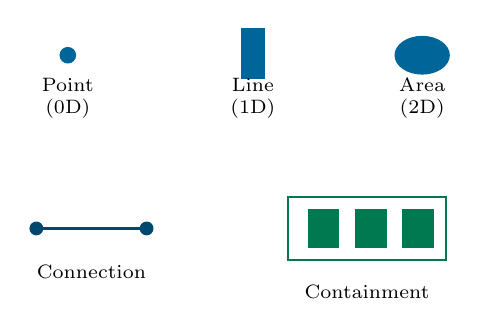
\begin{tikzpicture}[font=\small, >=Stealth]
  % Top row: item marks -- point, line, area
  % Point (0D)
  \fill[tuwblue] (0.8,1.5) circle (3pt);
  \node[font=\scriptsize, align=center] at (0.8,0.95) {Point\\(0D)};
  % Line (1D) -- a bar
  \fill[tuwblue] (3.0,1.2) rectangle (3.3,1.85);
  \node[font=\scriptsize, align=center] at (3.15,0.95) {Line\\(1D)};
  % Area (2D) -- a filled blob
  \fill[tuwblue] (5.3,1.5) ellipse (10pt and 7pt);
  \node[font=\scriptsize, align=center] at (5.3,0.95) {Area\\(2D)};

  % Bottom row: link marks -- connection, containment
  % Connection: two nodes joined by an edge
  \fill[tuwdark] (0.4,-0.7) circle (2.5pt);
  \fill[tuwdark] (1.8,-0.7) circle (2.5pt);
  \draw[thick, tuwdark] (0.4,-0.7) -- (1.8,-0.7);
  \node[font=\scriptsize, align=center] at (1.1,-1.25) {Connection};
  % Containment: big box with small boxes nested
  \draw[thick, keygreen] (3.6,-1.1) rectangle (5.6,-0.3);
  \fill[keygreen] (3.85,-0.95) rectangle (4.25,-0.45);
  \fill[keygreen] (4.45,-0.95) rectangle (4.85,-0.45);
  \fill[keygreen] (5.05,-0.95) rectangle (5.45,-0.45);
  \node[font=\scriptsize, align=center] at (4.6,-1.5) {Containment};
\end{tikzpicture}
\end{center}
\sketchnote{three rows of icons -- top: a dot (point/0D), a bar (line/1D), a
filled blob (area/2D); bottom: two nodes joined by an edge (connection) and a
big box with small boxes nested inside (containment).}

\subsection{Channels and the magnitude vs.\ identity split}

A \term{visual channel} is a way to control mark appearance, \emph{independent}
of mark dimensionality. The human perceptual system has two fundamentally
different sensory modalities, which splits all channels into two families:

\begin{keybox}[The fundamental split]
\term{Identity / "what--where" channels} (psychophysics: \emph{metathetic})
answer "what is it / where is it?" -- e.g.\ shape, color hue, spatial region,
motion pattern. They suit \term{categorical} attributes. \\[2pt]
\term{Magnitude / "how-much" channels} (psychophysics: \emph{prothetic}) answer
"how much is there?" -- e.g.\ length, area, volume, luminance, saturation, tilt,
position. They suit \term{ordered} (ordinal + quantitative) attributes.
\end{keybox}

\paragraph{List of channels.} Spatial: \term{aligned (common-scale) position},
\term{unaligned position}, \term{depth} (3D position), \term{spatial region}.
Color: \term{hue}, \term{saturation}, \term{luminance}. Size (one per added
dimension): \term{length} (1D), \term{area} (2D), \term{volume} (3D). Motion:
\term{motion pattern}, \term{direction}, \term{velocity}. Plus \term{angle/tilt},
\term{curvature}, and \term{shape} (a complex phenomenon treated as one channel).

\subsection{The two guiding principles}

\begin{keybox}[Expressiveness \& Effectiveness (Mackinlay 1986)]
\textbf{Expressiveness:} the encoding should express \emph{all of, and only,}
the information in the data. Ordered data must be shown so the perceptual system
senses order; unordered data must \emph{not} imply an order that does not exist.
$\Rightarrow$ \emph{match channel type to attribute type}. \\[3pt]
\textbf{Effectiveness:} the \emph{importance} of an attribute should match the
\emph{salience} (noticeability) of its channel. $\Rightarrow$ \emph{most
important attribute $\to$ most effective channel}; less important attributes get
less effective channels.
\end{keybox}

\begin{pitfall}[Classic expressiveness violation]
Encoding an unordered categorical attribute (e.g.\ country) with an ordered
magnitude channel (e.g.\ luminance or length) implies a ranking that does not
exist. This is "a common beginner's mistake." The reverse -- categorical hue
for a quantitative attribute -- destroys perceived order. In both cases the
expressiveness principle is violated even if the chart "works."
\end{pitfall}

\subsection{Channel effectiveness rankings}

Combining the two principles yields two ranked lists (Munzner Fig.~5.6), most
effective at the top. Spatial channels top \emph{both} lists and are the only
ones effective for both data types -- choosing what to encode with position is
the single most central encoding decision, because position-encoded attributes
dominate the user's mental model.

\begin{center}
\begin{tabular}{@{}r l l@{}}
\toprule
Rank & \textbf{Magnitude (ordered)} & \textbf{Identity (categorical)} \\
\midrule
1 & Position on common scale (aligned) & Spatial region \\
2 & Position on unaligned scale        & Color hue \\
3 & Length (1D size)                   & Motion \\
4 & Tilt / angle                       & Shape \\
5 & Area (2D size)                     & \\
6 & Depth (3D position)                & \\
7 & Color luminance                    & \\
8 & Color saturation                   & \\
9 & Curvature                          & \\
10 & Volume (3D size)                  & \\
\bottomrule
\end{tabular}
\end{center}

\noindent Note: luminance and saturation are roughly equally effective, as are
curvature and volume at the bottom.

\subsection{Accuracy: Cleveland \& McGill and Stevens}

\paragraph{Cleveland \& McGill (1984) accuracy ranking.} Controlled experiments
on the magnitude channels gave an empirical ordering of elementary perceptual
tasks, from most to least accurate:
\begin{enumerate}[label=\arabic*.]
  \item Position along a common scale (aligned)
  \item Position along identical, non-aligned scales (unaligned)
  \item Length
  \item Angle / slope
  \item Area
  \item Volume $\approx$ Curvature $\approx$ Luminance (equivalence class)
  \item Color hue \emph{(as a magnitude channel -- last; very different from its
        2nd place as an identity channel)}
\end{enumerate}
Heer \& Bostock (2010) replicated this by crowdsourcing; the one discrepancy is
that \emph{length and angle judgements turned out roughly equivalent}. These
accuracy results are the primary basis for the channel rankings above.

\paragraph{Stevens' power law.} Psychophysics shows that the apparent magnitude
$S$ of a sensory channel follows a power function of the physical intensity $I$:
\[
  S = I^{\,n}.
\]
The exponent $n$ depends on the modality and ranges from sublinear $0.5$
(brightness) to superlinear $3.5$ (electric current).
\begin{itemize}
  \item $n = 1$ (\term{length}): perception is accurate -- doubling the stimulus
        doubles the perception.
  \item $n < 1$ \term{compressive} (e.g.\ \term{area} $\approx 0.7$,
        \term{brightness} $\approx 0.5$): the channel is perceptually
        \emph{compressed} $\Rightarrow$ users \emph{underestimate} large values.
        Doubling brightness looks much less than twice as bright.
  \item $n > 1$ \term{expansive} (e.g.\ red--gray \term{saturation}, electric
        current): the channel is \emph{magnified} $\Rightarrow$ users
        \emph{overestimate}.
\end{itemize}

\begin{keybox}[Why position beats length -- Weber's Law]
Perception is fundamentally \emph{relative}, not absolute (\term{Weber's Law}:
$\delta I / I = K$). Unframed, unaligned bars are hard to compare; adding a
\emph{common frame} or \emph{alignment} gives a common scale, turning a hard
length judgement into an easy position judgement. This is why aligned position
on a common scale ranks first.
\end{keybox}

\subsection{Channel characteristics}

Effectiveness is analysed along five criteria: accuracy, discriminability,
separability, popout, and grouping.

\paragraph{Discriminability.} How many distinguishable \term{bins} (steps) does
a channel provide? The number of attribute values shown must not exceed the
channel's bin count. Example: \term{line width} has very few bins -- great for
3--4 values, poor for hundreds (it starts looking like an area). If they
mismatch, aggregate the attribute or pick another channel.

\paragraph{Separability vs.\ integrality.} Channel pairs lie on a continuum from
\term{separable} (can be attended independently) to \term{integral}
(inextricably fused; the brain perceives an unanticipated combination).

\begin{center}
\begin{tabular}{@{}l l l@{}}
\toprule
Channel pair & Interference & Result \\
\midrule
Position $+$ hue            & none (fully separable) & two clean groupings \\
Size $+$ hue                & some                   & hue hard to read on small marks \\
Width $+$ height            & significant (integral) & fused into perceived \emph{area} (small/med/large) \\
Red $+$ green (RGB axes)    & major (integral)       & perceived as one combined color \\
\bottomrule
\end{tabular}
\end{center}

\noindent Integral is not "bad": horizontal$+$vertical size is a \emph{good}
choice if you want a single attribute with three groups (small, flattened,
large). Match the pair's character to the information.

\paragraph{Popout (preattentive processing).} A distinct item "pops out" from
distractors in time \emph{independent of the number of distractors} -- our
low-level visual system processes the channel in massively parallel fashion
(also called preattentive / tunable detection). Channels supporting popout
include color hue, shape, tilt, size, proximity, motion, shadow direction.
\begin{pitfall}[Popout does not combine]
Popout works for \emph{one channel at a time}. A red circle does \emph{not} pop
out from a field mixing \{red, blue\} $\times$ \{circle, square\} -- it requires
\term{serial search} (time grows linearly with distractors). A few pairs are
exceptions (space$+$color, motion$+$shape); never count on popout for three or
more channels. Also, parallelism is \emph{not} preattentive.
\end{pitfall}

\paragraph{Grouping.} Strength of perceptual grouping cues, strongest first:
\term{containment} (area) $>$ \term{connection} (line) $>$ \term{proximity}
(spatial region) $>$ \term{similarity} (hue, motion, carefully chosen shape).
This proximity strength is exactly why spatial region is the top categorical
channel. Use shape and motion with care: a forward vs.\ backward "C" does not
form a selectable group, while circle vs.\ star does.

\subsection{Channel interference \& redundant encoding}

Two ideas often confused:
\begin{itemize}
  \item \term{Interference} -- encoding \emph{different} attributes in
        non-separable channels (size$+$hue, width$+$height) so the user cannot
        recover each attribute. Avoid.
  \item \term{Redundant encoding} -- encoding \emph{one} attribute in
        \emph{two} channels at once (e.g.\ both hue \emph{and} shape, or both
        position \emph{and} color) to make it very easily perceived. The cost is
        that channels are "used up," so fewer total attributes can be shown.
\end{itemize}

\begin{exambox}[How this is examined]
\textbf{Visualization Critique (open question).} Given a chart, you must:
\begin{itemize}[leftmargin=1.4em]
  \item Decompose it into \emph{marks} and \emph{channels} per attribute.
  \item Check \emph{expressiveness}: is each attribute's channel type matched to
        its data type? Flag categorical-on-magnitude (false order) or vice versa.
  \item Check \emph{effectiveness}: is the most important attribute on the most
        effective channel (position $>$ length $>$ angle $>$ area $>$ color)?
  \item Invoke \emph{Stevens' power law} to argue over/underestimation: area
        ($n\approx0.7$) and brightness ($n\approx0.5$) are underestimated;
        saturation is overestimated; length ($n=1$) is accurate.
  \item Spot \emph{channel interference} (e.g.\ width vs.\ height read as area;
        small marks make hue unreadable) and suggest separable alternatives or
        redundant encoding.
\end{itemize}
\textbf{MCQ on channel properties.} Be ready to: classify a channel as magnitude
vs.\ identity; order channels by effectiveness; recall the Cleveland \& McGill
ranking; identify separable vs.\ integral pairs; state which channels support
popout; and distinguish redundant encoding from interference.
\end{exambox}

\begin{pitfall}[Common confusions to avoid]
Hue is \emph{2nd} as an identity channel but \emph{last} as a magnitude channel.
"Position on a common scale" $\neq$ "length" -- the frame/alignment is what makes
position more accurate (Weber's Law). Effectiveness $=$ importance$\to$salience;
expressiveness $=$ data type$\to$channel type. Do not mix them up.
\end{pitfall}

\section{Perception and Color}

Visualization works because it offloads cognition onto the human \term{visual
system}, a high-bandwidth, partly pre-cognitive channel. Knowing how the eye
and early vision behave tells us \emph{which} visual channels are fast,
accurate and orderable, and which ones (notably hue) are not. This section
grounds the design rules used elsewhere (expressiveness, effectiveness, channel
ranking) in perception, and then covers color, the single most over-used and
most-often-misused channel in the exam's ``Visualization Critique'' questions.

\begin{keybox}[Why perception matters for vis]
A good encoding lets the visual system answer the task \emph{pre-attentively}
(in a glance, $\sim$200\,ms) instead of forcing slow serial reading.
Bad encodings (rainbow color, 3D bars, hue for ordered data) fight the visual
system and force slow, error-prone interpretation.
\end{keybox}

\subsection{The Human Visual System}

\subsubsection{Eye, retina, rods and cones}
Light from the scene is projected by the cornea/lens onto the \term{retina} at
the back of each eye. The retina is covered with photoreceptors:
\begin{itemize}
  \item \term{Cones} -- color-sensitive (three types, tuned to long / medium /
    short wavelengths), concentrated in the centre of the retina; responsible
    for detailed, color daytime vision.
  \item \term{Rods} -- highly light-sensitive but \emph{not} color-sensitive;
    dominate peripheral and low-light vision.
\end{itemize}

\subsubsection{Fovea and acuity}
The \term{fovea} is the small central region of the retina where image detail
and color rendition are best (densest cone packing). Crucially, the fovea
covers a viewing angle of only about \textbf{$2^\circ$} -- roughly a thumbnail
held at arm's length. Moving outward through the \term{parafovea} to the
\term{periphery}, \term{visual acuity} (the ability to resolve detail)
\emph{falls off dramatically} [Spence, Sec.~4.1].

\subsubsection{Fixations and saccades}
Because only a tiny region is seen in detail, the eye constantly jumps around
the scene. Each \term{fixation} (gaze held on one point) lasts about
\textbf{200\,ms}; fixations are connected by very fast ($\sim$20\,ms)
\term{saccades}. Viewing a whole image involves $\sim$100 fixations.
\term{Overt attention} is paid to a few fixated points; \term{covert
attention} to parafoveal/peripheral items helps decide where to look next.

\subsubsection{Visual cortex (it's complicated)}
Retinal signals pass through the LGN to the primary visual cortex \term{V1}
(the main entry point; neurons highly selective for gradients, i.e.\ ``edge
detection''), then V2/V4 with increasingly complex response, up to the inferior
temporal cortex (object recognition, memory). Exam-relevant takeaway:
\emph{luminance contrast drives edge detection}, which is why luminance is a
good channel for fine spatial detail and hue is not.

\sketchnote{Retina disk with a small bright dot labelled \emph{fovea}
($2^\circ$), a ring \emph{parafovea}, and an outer ring \emph{periphery}; an
arrow ``acuity'' pointing outward and shrinking. Beside it: a zig-zag gaze path
(fixations $\approx$200\,ms, saccades $\approx$20\,ms).}

\subsection{Preattentive Processing and Popout}

A \term{limited} set of visual channels is detected \emph{rapidly and in
parallel}, within $\sim$200--250\,ms, before focused attention engages.

\begin{keybox}[Operational definition (exam-quotable)]
If finding a target takes a \textbf{fixed amount of time regardless of the
number of distractors}, the channel is processed \term{preattentively}.
The target then ``pops out''.
\end{keybox}

A single red dot among blue dots pops out instantly whether there are 12 or 50
distractors. Channels that support popout include color (hue), orientation
(tilt), size, curvature, motion, and others (Healey's catalogue).

\begin{pitfall}[Conjunction search -- the key limitation]
Popout works only when the target differs in \emph{one} unique visual property.
If the target shares each of its properties with some distractors and is
defined only by a \term{combination} of features (e.g.\ ``the red \emph{circle}''
among red squares and blue circles), there is no unique channel to search for.
This is a \term{conjunction search}: \textbf{not possible pre-attentively}, so
a slow \emph{serial} search is required and search time grows with item count.
\end{pitfall}

\textbf{Important nuance:} a conjunction of \emph{spatial position} with one
other channel (color or shape) \emph{can} still be searched preattentively --
e.g.\ in a scatterplot the conjunction of space~$\times$~color, or
space~$\times$~shape, pops out. The hard case is conjunctions of two
non-spatial channels.

\begin{exambox}[How this is asked]
``Why is it slow to find X in this chart?'' $\Rightarrow$ identify whether the
target has a unique preattentive feature or requires conjunction search.
Design fix: encode the target's category with a \emph{single} popout channel
(e.g.\ make the outliers a distinct hue) so they pop out preattentively.
\end{exambox}

\subsection{Gestalt Laws of Grouping}

\term{Gestalt laws} describe how we perceive \term{patterns / groupings} in
visual displays, and translate directly into design principles for information
displays.

\begin{longtable}{@{}p{2.6cm}p{7.2cm}p{4.4cm}@{}}
\toprule
\textbf{Law} & \textbf{We group items that\ldots} & \textbf{Vis example} \\
\midrule
\endhead
Proximity     & are close together in space            & clusters in a scatterplot read as groups \\
Similarity    & look alike (same hue/shape/size)        & same-color points = same category \\
Connectedness & are joined by lines                     & node--link edges, slope graphs \\
Continuity    & lie along a smooth continuous contour   & a line is followed through crossings \\
Closure       & form a closed/implied contour           & we ``complete'' a shape \\
Symmetry      & are symmetric about an axis             & mirrored layouts read as one object \\
Common fate   & move together                           & animated points moving together group \\
Common region & lie inside a shared enclosure           & a shaded hull / bounding box \\
\bottomrule
\end{longtable}

\begin{keybox}[Which is strongest?]
\term{Connectedness} (and shared enclosure / common region) can be a
\emph{more powerful} grouping cue than \term{proximity}: items joined by a
line or surrounded by a hull are grouped even when other cues (color or
distance) would group them differently. The slides state explicitly:
\emph{``connectedness can be a more powerful grouping principle than
proximity.''}
\end{keybox}

\sketchnote{Two scatter clusters. (a) proximity alone $\to$ two groups by
distance. (b) draw a connecting line / shaded blob that links one point from
the left cluster to the right cluster $\to$ it now reads as belonging to the
enclosed group, overriding proximity.}

\subsection{Weber's Law and the Just Noticeable Difference}

\subsubsection{JND}
The \term{Just Noticeable Difference (JND)} is the amount a stimulus must be
changed to be detectable by human observers \emph{at least half of the time}.
It is determined \emph{empirically}.

\subsubsection{Weber's law}
The JND is \emph{not} an absolute amount: it is proportional to the background
stimulus magnitude. To perceive a difference between a background intensity
$I$ and the background plus stimulation $\Delta I$, the difference must be
proportional to the background:
\[
  k = \frac{\Delta I}{I} \quad\Longleftrightarrow\quad \Delta I = k\,I,
  \qquad k = \text{const (Weber fraction)}.
\]
\textbf{Implication:} we judge \emph{relative}, not absolute, differences.
Adding 5 dots to a field of 10 is obvious; adding 5 to a field of 100 is not,
even though the absolute change is identical.

\begin{keybox}[Consequences for design]
\begin{itemize}
  \item Integrating Weber's law over stimulus intensity gives \term{Fechner's
    law}: perceived intensity is \emph{logarithmic},
    $p = k\ln(I/I_0)$, where $I_0$ is the absolute threshold.
  \item More generally, \term{Stevens' power law} models perceived sensation
    as $p = k\,I^{\,a}$ ($a$ a measured exponent per channel). Length
    $a\!\approx\!1$ (perceived $\approx$ veridical); area $a\!\approx\!0.7$ and
    brightness $a\!\approx\!0.5$ are \emph{compressed} (under-estimated), while
    saturation and electric shock are exaggerated. This is the perceptual basis
    for why \emph{position/length beats area/color} in the channel ranking.
  \item Practical rule: length differences are most accurately judged when bars
    share a \textbf{common baseline and are adjacent}; offset or stacked bars
    make comparison much harder.
\end{itemize}
\end{keybox}

\subsection{Color}

\subsubsection{Color is three channels}
Colloquial ``color'' is best understood as \textbf{three separate channels}:
\term{luminance} (light--dark), \term{hue} (red, green, blue, \ldots), and
\term{saturation} (vividness). The major colormap design choice is which of
these to use for what.

\begin{keybox}[Ordered vs.\ unordered channels (Munzner)]
\begin{itemize}
  \item \term{Luminance}: a \emph{magnitude} (ordered) channel -- people
    reliably order grays, always placing gray between black and white.
  \item \term{Saturation}: ordered, but \emph{less easily} (only $\sim$3--4
    discriminable steps for small marks).
  \item \term{Hue}: an \emph{identity} (categorical, \textbf{unordered})
    channel. Asked to order red/blue/green/yellow patches, people disagree.
    \textbf{Hue cannot be ordered} -- learned conventions (rainbow, traffic
    lights) are higher-level, not perceptual.
\end{itemize}
\end{keybox}

\subsubsection{Opponent color theory}
The retina's signals are immediately processed into \textbf{three opponent
color channels}: red--green, blue--yellow, and a black--white channel encoding
\term{luminance}. The luminance channel carries \emph{high-resolution} edge
information; the two chromatic channels are \emph{lower resolution}. This is
why luminance (not hue) should carry fine spatial detail.

Opponent theory also explains \term{color blindness} (more accurately
\emph{color vision deficiency}), affecting $\sim$8--10\% of men in its common
form: the \term{red--green} channel is reduced/absent while blue--yellow still
works $\Rightarrow$ \textbf{avoid red--green encodings}.

\subsubsection{Colormap types and when to use each}
The colormap taxonomy mirrors the data-type taxonomy.

\begin{longtable}{@{}p{2.9cm}p{2.4cm}p{8.7cm}@{}}
\toprule
\textbf{Colormap} & \textbf{Data} & \textbf{Use / rule} \\
\midrule
\endhead
\term{Categorical} (qualitative) & categorical &
  Distinct hues for unordered groups; \emph{segmented}. Hue = identity channel.
  Limited to \textbf{$\sim$6--12 discriminable bins} (12 max). Requires a
  \textbf{legend}. \\
\term{Sequential} & ordered (ord./quant.) &
  Progression from min to max along an ordered channel (luminance, possibly
  with one hue), e.g.\ light$\to$dark pink. \\
\term{Diverging} & ordered with meaningful midpoint &
  Two sequential ramps meeting at a \textbf{neutral midpoint} (zero / mean),
  e.g.\ blue--white--red ``warming stripes''. Use when a zero/reference point
  is meaningful (gain vs.\ loss). \\
\term{Bivariate} & two attributes &
  Encodes two attributes at once. Easy to read when the 2nd attribute is
  \emph{binary}; quickly unreadable when both have several levels. \\
\bottomrule
\end{longtable}

Colormaps can be \term{continuous} (good for quantitative / spatial fields) or
\term{segmented}/binned (good for categorical; emphasizes discrete bins).

\begin{keybox}[Rules for categorical color]
\begin{itemize}
  \item Use \textbf{$\le$ 6--12} colors; more than 12 hues are very hard to
    discriminate (Ware). Count the background and default object colors
    (black/white/gray) in your budget.
  \item Prefer \textbf{easily nameable} colors (only $\sim$8 are consistently
    named): start with the opponent-axis colors red/green/blue/yellow, then
    orange/brown/pink/purple/cyan.
  \item Match saturation to mark size: \emph{small} marks (points, lines)
    $\to$ highly saturated; \emph{large} areas $\to$ low saturation/pastel.
  \item If categories exceed the color budget, aggregate into groups or an
    ``other'' bin, or switch to an additional channel (shape, size).
  \item Categorical color always needs a \textbf{legend}.
\end{itemize}
\end{keybox}

\subsubsection{The rainbow / jet colormap problem}
Using the rainbow (``jet'') colormap for \emph{ordered} data is a classic
mistake. Munzner lists three serious perceptual problems:

\begin{pitfall}[Three problems with the rainbow colormap]
\begin{enumerate}
  \item \textbf{Hue is used to indicate order}, but hue is an identity channel
    with \emph{no implicit perceptual ordering} (expressiveness mismatch).
  \item \textbf{Not perceptually uniform}: equal steps in data are \emph{not}
    perceived as equal -- some ranges show several distinct colors, others
    look uniform (a wide band that just ``looks yellow'').
  \item \textbf{Fine detail is lost}: hue cannot convey fine-grained detail;
    luminance would, because luminance contrast drives edge detection.
\end{enumerate}
Add a fourth, practical one: rainbow is \textbf{not color-blind safe}
(red/green confusions).
\end{pitfall}

\subsubsection{Perceptually uniform maps (viridis)}
The fixes: (i) design \term{monotonically increasing luminance} colormaps so
that order is carried by the magnitude (luminance) channel while hue only marks
semantic regions; (ii) use a \textbf{perceptually uniform} colormap such as
\term{viridis} -- built in a perceptually uniform space (cf.\ CIE
$L^*a^*b^*$) so equal data steps look equally different, with monotonic
luminance, and it is color-blind friendly. (A perceptually linear rainbow is
possible but loses brightness/dynamic range, so it is rarely used.)

\begin{exambox}[Color critique checklist]
For any color encoding, ask:
(1) Is the data \emph{ordered}? If yes, do \emph{not} use hue alone -- use
luminance / a sequential or diverging map.
(2) Is there a meaningful midpoint? $\to$ diverging.
(3) Categorical with $\le$12 groups? $\to$ distinct nameable hues + legend.
(4) Is it color-blind safe (no red--green dependence; redundant encoding)?
(5) Is it perceptually uniform (avoid rainbow/jet; prefer viridis)?
\end{exambox}

\begin{pitfall}[color $\neq$ color]
``Color'' is not one thing. Saying ``encode this with color'' is too vague:
state \emph{which} channel (luminance/hue/saturation) and check it matches the
attribute type (ordered $\to$ luminance; categorical $\to$ hue).
\end{pitfall}

\section{Design Principles and Visualization Critique}

This section is the toolkit for the exam's recurring \emph{``What is wrong with
this visualization? Suggest an improvement''} questions. It collects
Tufte-style integrity rules and Munzner's encoding rules, then gives a reusable
\term{critique checklist} and two fully worked critiques (a rainbow choropleth
and area-encoded circles). The golden rule underneath everything:
\term{function before form} -- start from the task (\emph{what} data,
\emph{why} task), then choose the encoding; never start from a pretty picture.

\begin{keybox}[Two governing principles (Munzner)]
\begin{itemize}
  \item \term{Expressiveness}: the visual structure should encode
    \emph{all and only} the information in the data. Ordered data must look
    ordered; unordered data must \emph{not} look ordered.
  \item \term{Effectiveness}: the most important attributes should get the most
    effective channels (faster to read, more distinctions, fewer errors).
    Spatial channels (position) are most effective.
\end{itemize}
\end{keybox}

\subsection{Data--Ink Ratio and Chartjunk (Tufte)}

\term{Data--ink} is the ink that encodes actual data. Tufte's
\term{data--ink ratio} is
\[
  \text{data--ink ratio} = \frac{\text{ink used to show data}}
                                 {\text{total ink used}}.
\]
\term{Chartjunk} is non-data ink that adds no information: heavy gridlines,
3D shading, decorative backgrounds, redundant frames, moir\'e patterns.

\begin{keybox}[Rules]
\textbf{Maximize the data--ink ratio} (within reason) and \textbf{erase
chartjunk}: remove or mute gridlines, drop 3D effects and shadows, avoid
decorative clipart. Every drop of ink should earn its place by conveying data.
\end{keybox}

\subsection{The Lie Factor (graphical integrity)}

Tufte's \term{lie factor} measures whether the visual effect matches the data:
\[
  \text{lie factor} = \frac{\text{size of effect shown in the graphic}}
                           {\text{size of effect in the data}}.
\]
``Size of effect'' $=$ (later value $-$ earlier value) $/$ earlier value, the
relative change. A lie factor of \textbf{1} is honest; $>1$ exaggerates,
$<1$ understates. Tufte considers $0.95$--$1.05$ acceptable.

\begin{exambox}[Worked computation]
A quantity grows from 18 to 27 in the data (effect $= (27-18)/18 = 0.50$, i.e.\
$+50\%$). The graphic draws bars whose \emph{heights} go from 1\,cm to 4\,cm
(shown effect $= (4-1)/1 = 3.0$, i.e.\ $+300\%$). Then
\[
  \text{lie factor} = \frac{3.0}{0.5} = 6.0,
\]
so the graphic exaggerates the change six-fold (a classic truncated-axis or
area-scaling lie).
\end{exambox}

\begin{pitfall}[Common lie-factor sources]
Truncated / non-zero baselines on bar charts; encoding a 1D value as 2D
\emph{area} (or 3D volume); inconsistent axis scaling. Always check the
baseline starts at zero for bars.
\end{pitfall}

\subsection{Over-Counting via Area (1D value as 2D size)}

When a single quantity is mapped to a circle, designers often scale the
\emph{radius} (or diameter) by the value. But the perceived magnitude is the
\term{area}, which then grows with the \emph{square} of the value:
double the value $\Rightarrow$ radius~$\times2$ $\Rightarrow$
area~$\times4$. The graphic over-states the difference fourfold.

\begin{exambox}[The ``men of talent'' circle example]
Tufte's classic case: circles sized to show a quantity were scaled by diameter,
so a value twice as large was drawn with $4\times$ the area -- a huge,
misleading exaggeration. \textbf{Rule:} if you must use circles, scale by
\emph{area} (value $\propto$ area, so radius $\propto \sqrt{\text{value}}$).
Even then, \emph{area is perceptually under-estimated} (Stevens exponent
$\approx 0.7$), so length/position bars are a better encoding for magnitude.
\end{exambox}

\begin{keybox}[Area perception cuts both ways]
\begin{itemize}
  \item \textbf{Mis-encoding} (radius scaling) over-states differences
    ($\times$value$^2$).
  \item \textbf{Perception} of correctly area-scaled marks \emph{under-states}
    differences (compression, exponent $<1$).
\end{itemize}
So area is doubly problematic: prefer length on a common scale for quantities.
\end{keybox}

\subsection{Ordering of Bars, Axes and Categories}

For \emph{unordered categorical} keys, the layout order is a free design
choice -- use it to carry information.

\begin{keybox}[Order by value, not by alphabet]
Sort bars / rows / categories by their \textbf{data value} (e.g.\ descending),
not alphabetically or by arbitrary ID. A value-sorted bar chart makes rank,
extremes and the distribution shape readable at a glance; an alphabetical order
hides them. For ordinal keys, keep the intrinsic order.
\end{keybox}

\subsection{Expressiveness Violations}

\begin{pitfall}[The most common beginner mistake]
\textbf{Showing ordered data with an unordered (identity) channel}, or
\textbf{implying an order that does not exist}.
\begin{itemize}
  \item Quantitative value on \emph{hue} (rainbow colormap) -- hue is an
    identity channel; it implies categories, not order.
  \item Categorical attribute on \emph{position on a continuous axis} -- implies
    an ordering the data does not have.
\end{itemize}
Fix: ordered attribute $\to$ magnitude channel (position, length, luminance);
categorical attribute $\to$ identity channel (hue, shape, spatial region).
\end{pitfall}

\subsection{Effectiveness, Stevens' Power Law and the Channel Ranking}

Effectiveness is grounded in perception (Stevens' power law: perceived
sensation $p = k\,I^{a}$; see the Perception section). Channels are split into
\term{magnitude channels} (for ordered attributes) and \term{identity
channels} (for categorical attributes), each ranked by accuracy.

\begin{longtable}{@{}p{6.7cm}p{6.7cm}@{}}
\toprule
\textbf{Magnitude (ordered), best$\to$worst} & \textbf{Identity (categorical), best$\to$worst} \\
\midrule
Position on common scale     & Spatial region \\
Position on unaligned scale  & Color hue \\
Length (1D size)             & Motion \\
Tilt / angle                 & Shape \\
Area (2D size)               & \\
Depth (3D position)          & \\
Color luminance, saturation  & \\
Curvature                    & \\
Volume (3D size)             & \\
\bottomrule
\end{longtable}

\begin{keybox}[Takeaways]
\textbf{Spatial (position) channels are the most effective} for both ordered
and categorical data. Put the most important attribute on position. Area, color
and especially volume are weak for magnitude.
\end{keybox}

\subsection{Channel Interference (separable vs.\ integral)}

When two attributes are encoded on two channels, the channels should be
\term{separable} -- selectively attendable -- so each can be read independently.
\term{Integral} channel pairs fuse perceptually and cannot be separated.

\begin{longtable}{@{}p{6.5cm}p{6.9cm}@{}}
\toprule
\textbf{Separable (good)} & \textbf{Integral (bad for 2 attributes)} \\
\midrule
Position + hue (fully separable) & Red + green (major interference) \\
                                 & Width + height (size dimensions fuse) \\
                                 & Size + hue (some interference) \\
\bottomrule
\end{longtable}

\begin{pitfall}[Channel interference]
Encoding two \emph{separate} attributes in an integral pair (e.g.\
red--green, or x-size~+~y-size) fails -- viewers see one fused blob, not two
attributes. Choose channels with as little interference as possible.
\end{pitfall}

\subsection{Eyes Beat Memory: Juxtaposition vs.\ Animation}

\begin{keybox}[Eyes beat memory]
Comparison is far more accurate when both items are visible \emph{at the same
time} (\term{juxtaposition} -- side-by-side small multiples) than when the
viewer must hold one in memory while looking at the other. \textbf{Animation
forces comparison through memory} and is therefore weak for precise comparison;
prefer side-by-side static views. (Redundant encoding -- using $>1$ channel for
the \emph{same} attribute -- is the opposite, and is fine: it aids robustness,
e.g.\ color $+$ symbol for color-blind safety.)
\end{keybox}

\subsection{Problems with 3D}

\begin{pitfall}[Unjustified 3D]
Adding a third spatial dimension to data that is not inherently 3D causes:
\begin{itemize}
  \item \textbf{Perspective distortion} -- equal data values map to unequal
    screen sizes depending on depth, so comparison is biased.
  \item \textbf{Occlusion} -- nearer marks hide farther ones; data is lost.
  \item \textbf{Shadows / shading} and reduced \textbf{text legibility}.
\end{itemize}
Slide rule: \emph{``No unjustified 3D!''} A 3D bar chart is almost always worse
than its 2D version.
\end{pitfall}

\begin{keybox}[When 3D \emph{is} justified]
Use 3D only for \term{inherently spatial} data where the third dimension
\emph{is} part of the data -- e.g.\ 3D medical/volume data, molecular
structures, terrain, fluid-flow fields. There the benefit of matching the data's
spatial nature outweighs the distortion/occlusion costs (and interaction such
as rotation mitigates them).
\end{keybox}

\subsection{Function Before Form}

\begin{keybox}[Process: What / Why / How]
Design follows the loop \term{What} (data abstraction) $\to$ \term{Why} (task
abstraction) $\to$ \term{How} (visual encoding + interaction). Decide the task
\emph{first}; the most expressive and effective encoding follows from it. A
chart that looks impressive but does not support the task fails.
\end{keybox}

\subsection{The Critique Checklist (use on any chart)}

\begin{exambox}[Step-by-step critique]
\begin{enumerate}
  \item \textbf{What \& Why}: what is the data type of each attribute
    (categorical / ordered / quantitative) and what is the task
    (identify / compare / summarize, trend / outlier / correlation)?
  \item \textbf{Expressiveness}: does each channel match its attribute type?
    (ordered$\to$magnitude, categorical$\to$identity). Any false ordering?
  \item \textbf{Effectiveness}: is the most important attribute on the most
    effective channel (position/length), not on a weak one (area/hue)?
  \item \textbf{Integrity}: zero baseline? lie factor $\approx 1$? 1D value not
    encoded as 2D area? axes consistent?
  \item \textbf{Color}: ordered data not on hue (no rainbow); diverging needs a
    midpoint; categorical $\le$12 nameable hues + legend; color-blind safe (no
    red--green); perceptually uniform (viridis)?
  \item \textbf{Channels}: separable, not integral? not too many channels at
    once?
  \item \textbf{Ordering}: bars/categories sorted by value, not alphabet?
  \item \textbf{Chartjunk \& 3D}: remove non-data ink; no unjustified 3D.
  \item \textbf{Comparison}: juxtaposed (eyes), not animated (memory)?
  \item \textbf{Then suggest a concrete fix} for each issue.
\end{enumerate}
\end{exambox}

\subsection{Worked Critique 1: Rainbow Choropleth (Texas map)}

\textit{Scenario:} a US state/county choropleth coloring a continuous
quantitative attribute (e.g.\ a per-county ratio) with the \term{rainbow / jet}
colormap.

\begin{keybox}[Critique]
\begin{itemize}
  \item \textbf{Expressiveness violation}: the value is \emph{ordered} but it is
    encoded with \emph{hue}, an unordered identity channel -- the legend order
    (pink, blue, green, yellow, orange\ldots) carries no perceptual order, so
    readers cannot tell which county is higher without constant legend
    lookups.
  \item \textbf{Not perceptually uniform}: equal value steps look unequal;
    some adjacent bins look identical while others jump.
  \item \textbf{Fine detail lost}: hue cannot resolve fine differences;
    luminance contrast (needed for edges) is missing.
  \item \textbf{Not color-blind safe}: red/green bins are confusable for
    $\sim$8--10\% of men.
\end{itemize}
\end{keybox}

\begin{keybox}[Fix]
Replace with a \textbf{sequential} colormap that uses \emph{luminance} (light
$\to$ dark, single or few hues), or a \textbf{perceptually uniform} map
(\term{viridis}); if there is a meaningful midpoint, use a \textbf{diverging}
map with a neutral centre. Use a \textbf{color-blind-safe} palette
(ColorBrewer), and keep the legend ordered by value.
\end{keybox}

\subsection{Worked Critique 2: Area-Encoded Circles}

\textit{Scenario:} two (or more) quantities shown as circles, with the
\emph{radius/diameter} proportional to the value (``men of talent'' style).

\begin{keybox}[Critique]
\begin{itemize}
  \item \textbf{Over-counting via area}: radius $\propto$ value makes
    \emph{area} $\propto$ value$^2$, so the bigger circle looks far larger than
    the data warrants (lie factor $>1$).
  \item Even with correct area scaling, \textbf{area is under-estimated}
    perceptually (Stevens exponent $\approx 0.7$): differences are hard to
    judge accurately.
  \item Comparing \emph{areas} of separated circles is a weak perceptual task
    (low on the channel ranking).
\end{itemize}
\end{keybox}

\begin{keybox}[Fix]
Encode the magnitude with \textbf{length / position on a common scale} -- a
\textbf{bar chart with a zero baseline}, bars adjacent and sorted by value.
This puts the value on the most effective channel, removes the squaring error,
and lets readers compare precisely. If circle sizing is unavoidable (e.g.\ a
bubble map), scale by \emph{area} (radius $\propto\sqrt{\text{value}}$) and add
direct value labels.
\end{keybox}

\begin{exambox}[Phrasing your answer]
A full-credit critique names the \emph{principle} (e.g.\ ``expressiveness
violation: ordered data on hue''), explains the \emph{perceptual reason}, and
gives a \emph{concrete fix} (``use a sequential luminance/viridis map''). Bullet
each issue; do not just say ``it looks bad''.
\end{exambox}

\section{Tasks and Interaction}

This section covers the \emph{why} of visualization (Munzner's task abstraction, ch.~3) and the \emph{how} of interaction (selection, brushing \& linking, overview+detail, focus+context, dynamic queries, coordinated multiple views, high-dimensional brushing after Ward, and quantitative visual analytics). The unifying idea from the lecture: \term{interaction is a cognitive amplifier}. Static visualization fails for large data, multiple questions, and evolving hypotheses; interaction lets one display answer many questions over time.

\begin{keybox}[The what--why--how chain (Munzner)]
Every analysis instance is described by three orthogonal questions:
\begin{itemize}
  \item \term{What} is shown -- the data abstraction (dataset and attribute types).
  \item \term{Why} is it used -- the \emph{task} abstraction: \term{actions} (verbs) on \term{targets} (nouns).
  \item \term{How} is it built -- the idiom: encode, manipulate, facet, reduce.
\end{itemize}
Key principle: \textbf{why does not dictate how} -- the same goal can be served by many idioms. Tasks are stated in \emph{abstract} (domain-independent) terms so that two domain tasks ("contrast patients\dots" vs. "see if results match\dots") are recognised as the same abstract task ("compare values between two groups"). Complex activities are a \term{chained sequence} of tasks: the output of one becomes the input of the next (e.g. a \emph{discover} session feeds a later \emph{present} session).
\end{keybox}

\subsection{Task Abstraction: Actions (Munzner ch.~3)}

Actions sit at three independent levels; usually you specify all three.

\subsubsection{High level -- Analyze (consume vs.\ produce)}
\begin{itemize}
  \item \term{Consume} existing information:
  \begin{itemize}
    \item \term{Discover} -- find new knowledge; \emph{generate} or \emph{verify} a hypothesis (the classic motivation for sophisticated interactive idioms; close to \emph{explore}).
    \item \term{Present} -- communicate something already understood to an audience (telling a story; decision support, teaching). Knowledge is known to the presenter in advance.
    \item \term{Enjoy} -- casual encounters driven by curiosity (e.g. Name Voyager).
  \end{itemize}
  \item \term{Produce} new material for later use:
  \begin{itemize}
    \item \term{Annotate} -- add graphical/textual notes to existing elements (an annotation tied to data items can be seen as a new attribute).
    \item \term{Record} -- save persistent artifacts (screenshots, bookmarks, parameter settings, interaction logs, a branching \emph{graphical history}); supports analytic provenance.
    \item \term{Derive} -- compute new data from existing data (a.k.a.\ \emph{transform}). The data abstraction is an \emph{active design choice}: "don't just draw what you're given -- decide the right thing to show and create it." E.g. plot $\textit{trade balance}=\textit{exports}-\textit{imports}$ directly instead of two curves.
  \end{itemize}
\end{itemize}

\subsubsection{Mid level -- Search (a 2$\times$2 of known/unknown)}
Classified by whether the \emph{target} (identity, the \emph{what}) and the \emph{location} (the \emph{where}) are known.

\begin{center}
\begin{tabular}{l l l}
\toprule
 & \textbf{Target known} & \textbf{Target unknown} \\
\midrule
\textbf{Location known}   & \term{Lookup}  & \term{Browse} \\
\textbf{Location unknown} & \term{Locate}  & \term{Explore} \\
\bottomrule
\end{tabular}
\end{center}

\noindent\emph{Lookup}: know what and where (look up "humans" in a known spot of a tree). \emph{Locate}: know what, not where (hunt for "rabbits"). \emph{Browse}: know roughly where, not exactly what (scan a subtree / a date column). \emph{Explore}: know neither -- start from an overview, hunt for outliers/anomalies. (The verb \term{find} is the generic synonym for a successful search.)

\subsubsection{Low level -- Query (scope: one / some / all)}
Once targets are found, query them at one of three scopes of increasing breadth:
\begin{itemize}
  \item \term{Identify} -- one target (return its characteristics, e.g. one US state's result).
  \item \term{Compare} -- some targets (multiple; typically harder, needs richer idioms).
  \item \term{Summarize} -- all targets. Synonym \term{overview}, extremely common in vis.
\end{itemize}

\subsection{Task Abstraction: Targets}
Targets are the aspect of the data of interest (nouns).
\begin{itemize}
  \item \term{All data}: \term{trends} (a.k.a.\ \emph{patterns}: increases, peaks, plateaus), \term{outliers} (anomalies, deviants, surprises), \term{features} (task-dependent structures).
  \item \term{One attribute}: an individual value, the \term{extremes} (min/max), or the whole \term{distribution}.
  \item \term{Multiple attributes}: \term{dependency} (one depends on another), \term{correlation} (tendency to co-vary), \term{similarity} (quantitative closeness across all values).
  \item \term{Network data}: \term{topology} (structure of interconnections) and \term{paths} between nodes.
  \item \term{Spatial data}: \term{shape}.
\end{itemize}

\sketchnote{Draw the Actions tree (Analyze$\to$Consume/Produce; Search 2$\times$2 table; Query: identify/compare/summarize) next to the Targets list (all-data / one-attr / many-attr / network / spatial). This single diagram answers most "name the task" exam questions.}

\subsection{Interaction Techniques}

A useful working definition (Card et al.): "The use of computer-supported, \emph{interactive}, visual representations of abstract data to amplify cognition." Why interact: encoding determines which questions are easy, and there is \term{no single best visualization} -- interaction lets the user switch encodings and ask new questions on the fly.

\begin{keybox}[Catalogue of techniques]
\textbf{Change visual encoding}: change arrangement (e.g.\ re-baseline a stacked bar chart for easier sub-section comparison), change marks/channels, change shown dimensions, reorder/sort. \\
\textbf{Selection \& highlighting}: mark items as interesting; highlight makes them stand out (color/emphasis). The most fundamental brush operation. \\
\textbf{Brushing \& linking}: select in one view $\rightarrow$ \emph{linked highlighting} in all views. \\
\textbf{Navigation}: pan/scroll and \textbf{zoom} (geometric vs.\ semantic). \\
\textbf{Details-on-demand}: show full record for an item when requested. \\
\textbf{Dynamic queries / filtering}: show items conditionally; interactive query refinement.
\end{keybox}

\subsubsection{Shneiderman's Visual Information-Seeking Mantra}
\begin{algobox}[Shneiderman 1996]
\begin{center}\itshape\large "Overview first, zoom and filter, then details on demand."\end{center}
\begin{itemize}
  \item \term{Overview} -- starting point; shows overall patterns; needed for navigation/orientation.
  \item \term{Zoom \& filter} -- narrow to a region of interest, hide irrelevant items.
  \item \term{Details on demand} -- inspect individual cases/variables only when asked.
\end{itemize}
\end{algobox}

\subsubsection{Zoom: geometric vs.\ semantic; pan}
\term{Geometric zoom} simply scales the view. \term{Semantic zoom} changes \emph{what} is shown / how items are rendered as scale changes (more or different content at finer levels), not just size. \term{Pan/scroll} provides a larger virtual screen but is clunky and shows only one piece at a time. Rule of thumb: a long pan is bad -- "zoom out, pan a little, zoom in."

\subsubsection{Overview+Detail vs.\ Focus+Context}
The \term{core problem}: large data needs both \emph{overview} (patterns) and \emph{detail} (inspection), but not both at full resolution at once. Zoom-in loses context, zoom-out loses detail, pan causes disorientation.
\begin{itemize}
  \item \term{Overview+detail} -- combine via \emph{space} (different screen regions for overview and detail) or via \emph{time} (alternate sequentially in the same place).
  \item \term{Focus+context (F+C)} -- integrate a (zoomed) focus and its context within \emph{one} view; "seeing detail without losing the big picture." Focus $=$ detail, context $=$ structure.
\end{itemize}

\paragraph{F+C design space (three families).}
\begin{itemize}
  \item \term{Distortion-oriented} -- bend space; like a \emph{fisheye lens}: center enlarged, periphery compressed, everything stays visible but not equally emphasized (e.g.\ Perspective Wall).
  \item \term{Views-/layers-based} -- separate views for focus and context (e.g.\ a small overview map / minimap, Macroscope).
  \item \term{In-place} -- no geometric distortion; emphasize via color, blur, transparency (e.g.\ Semantic Depth of Field, SDOF).
\end{itemize}

\paragraph{Fisheye terminology (Furnas).} A fisheye view is computed from:
\begin{itemize}
  \item \term{Focal point} -- the item/coordinate the user focuses on.
  \item \term{Level of Detail (LoD)} -- intrinsic a-priori importance of each data element.
  \item \term{Distance from focus} -- how far an item is from the focal point.
  \item \term{Degree-of-Interest (DOI) function} -- governs how each item is rendered, e.g.
  \[
    \text{DOI}(item) = \text{LoD}(item) - \text{Distance}(item,\,focus).
  \]
\end{itemize}
DOI can be \emph{continuous} (smooth interpolation), \emph{filtering} (items past a threshold disappear), \emph{stepped} (discrete regions), or \emph{semantic} (rendering changes type at different levels).

\begin{keybox}[Why F+C matters / trade-offs]
\textbf{Benefits}: maintains orientation, reduces navigation effort, supports exploration; aligns well with the information-seeking mantra and data drill-down; also usable for presentation (SDOF). \emph{Requires interaction} (focusing, navigation) with smooth changes -- it is dynamic, not static. \\
\textbf{Trade-offs}: distortion $\rightarrow$ spatial confusion; layers $\rightarrow$ split attention; in-place $\rightarrow$ limited expressiveness.
\end{keybox}

\subsubsection{Response-time budget}
$\le 100$\,ms feels \emph{instantaneous}; $\le 1$\,s feels like \emph{free interaction}; $> 10$\,s loses the user's attention entirely (Card, Robertson \& Mackinlay 1991). Justifies why interactive idioms must keep latency low.

\subsubsection{Seven categories of interaction (Yi et al.\ 2007)}
A complementary taxonomy phrased as user intents: \term{Select} ("mark as interesting"), \term{Explore} ("show something else"), \term{Reconfigure} ("different arrangement"), \term{Encode} ("different representation"), \term{Abstract/Elaborate} ("more or less detail"), \term{Filter} ("show conditionally"), \term{Connect} ("show related items").

\subsection{Linked Views / Coordinated Multiple Views (CMV)}
\begin{keybox}[Why linking is crucial]
A single 2D view cannot show all attributes of a multidimensional table. CMV shows \emph{various attributes simultaneously in several simple 2D views} (parallel coordinates, scatterplot matrix, histograms, box plots, \dots). \term{Brushing \& linking} ties them together: \textbf{select items in one view and they are highlighted in all views}. This reveals how a feature in one attribute relates to others -- e.g.\ which items are extreme in $X$ \emph{and} where they fall in $Y,Z,\dots$ Interaction (not a fancy single chart) is what makes multidimensional analysis tractable.
\end{keybox}

Open questions raised in the lecture for CMV/brushing: brushing \emph{reproducibility}, communicating results, keeping focus on analysis (not on fiddling with the interaction), whether brushing is always best, and how to improve it.

\subsection{High-Dimensional Brushing (Ward, XmdvTool)}

Traditionally brushes live in \emph{screen space} (paint/rubber-band a 2D region). Ward's contribution: \term{N-dimensional brushes defined in data space} rather than screen space, integrated into XmdvTool (which shows the same multivariate data via scatterplot matrices, star glyphs, parallel coordinates, and dimensional stacking).

\begin{keybox}[Brush specification \& operations]
\textbf{Specification (redundant on purpose):} direct manipulation (drag/resize the brush boxes per display) or indirect via the \emph{brush toolbox} (global resize: max/half/$\pm$10\%). \\
\textbf{Brush structure:} a brush is a \emph{hyperbox} -- an extent (start..end) in each of the $N$ dimensions. \\
\textbf{Per-display manipulation:} scatterplot (drag boxes in each plot of the $N\times N$ matrix), parallel coordinates (sliders on each axis), glyph and dimensional-stacking brush tools. \\
\textbf{Brush operations:} highlighting, linking (default across all views), masking/deleting, moving average, quantitative (numeric) display.
\end{keybox}

\paragraph{Data-driven brushing ("painting").} Instead of setting bounds by hand in every dimension, the user \emph{paints} over data points of interest (shift+drag); a brush hyperbox is generated as the min/max along each axis of the painted points -- the \emph{data} drives the brush. Useful when bounds are unknown in dense data. (Demand-driven brushing $=$ the user specifies criteria, e.g.\ high in dim 1, low in dim 2, any in dim 3.)

\paragraph{Compound / composite brushes.} Multiple brushes (XmdvTool supports four) combined with \term{boolean operators} AND, OR, XOR, NOT. With ramped (non-binary) coverage the operators become arithmetic on coverage $C\in[0,1]$:
\[
  C_{\text{OR}}=\max(C_A,C_B),\quad
  C_{\text{AND}}=\min(C_A,C_B),\quad
  C_{\text{XOR}}=1-\lvert 1-(C_A+C_B)\rvert .
\]

\paragraph{Brush boundaries / extents.} Containment is usually binary (\emph{stepped} boundary). A \term{ramped} boundary linearly drops coverage from 1 (inside, at the inner boundary) to 0 (outside) between an inner and outer boundary -- distinguishing data near the brush center from data near its edge.

\paragraph{Structure-based brushing.} Brushing on a \emph{hierarchical/structural} representation of the data (e.g.\ a cluster tree) rather than on raw value extents -- select by structure, not just by per-dimension ranges.

\begin{pitfall}[Brushing exam traps]
Do not say a Ward brush is a screen-space rectangle -- its key novelty is that it is an \emph{N-dimensional hyperbox in data space}. Do not confuse \emph{data-driven} (paint the points, bounds inferred) with \emph{demand-driven} (state the criteria up front). AND $=\min$, OR $=\max$ for ramped coverage (not the other way round).
\end{pitfall}

\subsection{Quantitative Visual Analytics (Rado\v{s} et al.\ 2016)}
The additional deck pushes interactive analysis from qualitative toward \term{reproducible and quantitative VA}, via four extension groups:
\begin{itemize}
  \item \term{Structured brushing} -- brushing characterised along three axes: \emph{brush anchoring}, \emph{brush extent}, \emph{brush movement}, each \emph{unconstrained}, \emph{constrained} (snapped to a grid of percentile cells), or \emph{automatic} (programmatic, reproducible) -- improving reproducibility.
  \item \term{Percentile brushes} -- circle/rectangle and \emph{Mahalanobis} brushes; the Mahalanobis brush takes the underlying data \emph{distribution / covariance} into account so a single click+drag matches an elongated cluster.
  \item \term{Linked statistics} -- overlay numeric summaries (mean, median, midrange, spread) directly on the view and in numerical tables, linking data to its statistics.
  \item \term{Change visualization} -- traces/graphs of how statistics evolve while refining a brush, plus a difference-plot; supports iterative \term{drill-down} and \emph{query refinement}.
\end{itemize}
Underlying tension highlighted in class: \emph{complex interaction $+$ simple data} vs.\ \emph{simple interaction $+$ complex (pre-derived/aggregated) data} -- data derivation/aggregation can be moved into the system (on-the-fly data generation).

\begin{exambox}[How this is asked]
\begin{itemize}
  \item \textbf{"Justify the interaction design"} (strategy questions): map each chosen technique to a task. State the \emph{why} (action $+$ target, e.g.\ \emph{explore} for \emph{outliers}; \emph{compare} \emph{distributions}), then pick the \emph{how} (overview first $\to$ filter $\to$ details-on-demand; F+C to keep orientation; CMV with linked highlighting). Remember \emph{why does not dictate how} and there is no single best vis -- argue trade-offs and the response-time budget ($<1$\,s).
  \item \textbf{"Map the data items to a task"}: classify with Munzner -- which \emph{action} (lookup/locate/browse/explore $\times$ identify/compare/summarize) on which \emph{target} (trend/outlier/distribution/correlation/topology/path/shape).
  \item \textbf{Brushing \& linking}: explain selecting in one view highlights the same items everywhere, and \emph{why} that is essential for multidimensional tables (relate a feature in one attribute to all others). For Ward: N-D hyperbox in data space, painting (data-driven), AND/OR/XOR/NOT composite brushes, ramped vs.\ stepped extents, structure-based brushing.
  \item \textbf{Focus+context}: name the three families (distortion / views-layers / in-place), the fisheye DOI $=$ LoD $-$ distance, and the trade-offs (distortion $\to$ confusion, layers $\to$ split attention).
\end{itemize}
\end{exambox}

\section{High-Dimensional Data Visualization}

High-dimensional data has \term{many attributes} (columns / dimensions / features /
variables) per item. A working definition from the lecture: data are
\term{high-dimensional} when our traditional visual encodings for tabular data
\emph{break} (Yang et al., 2003) -- typically already from dozens of dimensions
on. Structured data has named, interpretable attributes (e.g.\ demographic
indicators, gene expression); unstructured data (text, images, audio) is turned
\emph{into} a high-dimensional feature matrix via bag-of-words /
document-term matrices, flattened pixels (MNIST $\to$ $784$-dim vector),
word embeddings (word2vec) or learned latent codes (autoencoders, CNNs).
Abstractly everything is a flat $n \times m$ table $X$ ($n$ items $\times$ $m$
attributes), only $m$ is very large and the attributes may not be interpretable.

\begin{keybox}[Two fundamental strategies]
\begin{itemize}
\item \term{Feature selection}: pick a \emph{subset} of the existing dimensions,
      \emph{without} transforming them. Axes stay interpretable. Dimensions (or
      dimension pairs) are ranked by a \term{quality metric} / ``cognostic''
      (computed diagnostic), then shown with 1D/2D/nD techniques.
\item \term{Feature extraction} (= dimensionality reduction): \emph{transform}
      existing features into a new, lower-dimensional space (project onto new
      axes). The new axes are usually \emph{not} interpretable, and extraction
      \emph{loses information}.
\item \term{Hybrid}: select fewer meaningful dimensions first (needs domain
      knowledge), then apply dimensionality reduction on them.
\end{itemize}
\end{keybox}

% =====================================================================
\subsection{Curse of Dimensionality (Giraud)}

As the dimension $p$ grows, high-dimensional spaces become \term{vast} and data
points get \term{isolated in their immensity}. Three intertwined effects:

\begin{itemize}
\item \term{Distance concentration}: the notion of ``nearest neighbor'' vanishes.
      For $n$ points sampled uniformly in $[0,1]^p$, as $p$ increases the
      \emph{minimal} distance between two points increases and \emph{all}
      pairwise distances become almost equal -- every point is roughly equally
      far from every other. The mean square distance grows linearly with $p$,
      $\mathbb{E}\!\left[\lVert X^{(i)}-X^{(j)}\rVert^2\right]=p/6$, while the
      \emph{relative} spread (scaled deviation) shrinks like $p^{-1/2}$. Any
      method based on \term{local averaging} (e.g.\ $k$-Nearest-Neighbors,
      kernel smoothing) therefore fails.
\item \term{Sparsity}: to keep observations within distance $1$ of any query
      point, the required number of samples $n$ grows \emph{more than
      exponentially} with $p$. The lower bound is
      $n \gtrsim \left(\tfrac{p}{2\pi e}\right)^{p/2}\!\sqrt{p\pi}$; e.g.\ for
      $p=100$ already $n \approx 4\cdot10^{39}$, for $p=200$ more than the
      estimated number of particles in the observable universe. Real data is
      hopelessly sparse in high-$p$ space.
\item \term{Vanishing volume}: the volume $V_p(r)$ of a $p$-ball goes to zero
      more than exponentially fast in $p$; for $p\approx20$ the unit ball is
      already almost $0$. Geometric intuitions from 2D/3D are misleading.
\item \term{Cumulating fluctuations}: accumulation of many small fluctuations
      across directions produces a large global fluctuation; rare events
      accumulate and may no longer be rare; computations/optimizations become
      intensive.
\end{itemize}

\begin{pitfall}[``More features is always better'']
The ``blessing'' of measuring thousands of variables is offset by the curse:
\emph{separating signal from noise is in general almost impossible} in
high-dimensional data. More dimensions $\neq$ more usable information.
\end{pitfall}

% =====================================================================
\subsection{Feature Selection vs.\ Feature Extraction (Ghojogh)}

Both reduce dimensionality: a mapping $\mathbf{x}\in\mathbb{R}^d \mapsto
\mathbf{y}\in\mathbb{R}^p$ with $p\le d$.

\begin{itemize}
\item \term{Feature selection}: $p\le d$ and the selected set
      $\{\mathbf{y}^j\}\subseteq\{\mathbf{x}^j\}$ is an \emph{inclusive subset} of
      the original features. Selection criterion improves/maintains accuracy or
      simplifies the model. There are $2^d$ possible subsets, so heuristics are
      used. Two evaluation philosophies:
      \begin{itemize}
      \item \term{Filter methods}: rank/score features \emph{independently} of any
            learning model, then threshold. Based on \term{relevance} (predictive
            power w.r.t.\ target) and \term{redundancy}. Measures: correlation
            criteria (Pearson), mutual information / information gain,
            $\chi^2$ statistics, Markov blanket, consistency-based filter, FCBF
            (symmetrical uncertainty), Interact, mRMR (max relevance, min
            redundancy). Fast, model-agnostic.
      \item \term{Wrapper methods}: \emph{integrate the model} into the subset
            search -- train and test the classifier on each candidate subset and
            use its performance as fitness. Search is NP-hard, so heuristic:
            sequential forward/backward selection (SFS/SBS, also floating
            SFFS/SFBS) or metaheuristics (genetic algorithms, particle swarm).
            More accurate but expensive; risk of overfitting to the model.
      \item \term{Embedded methods}: selection happens \emph{during} model
            training (e.g.\ LASSO / regularization, tree importances). Between
            filter and wrapper in cost.
      \end{itemize}
\item \term{Feature extraction}: the new set $\{\mathbf{y}^j\}$ is \emph{not} a
      subset but a \emph{different space} (projection to new axes); often
      $p\ll d$. Relies on the \term{manifold hypothesis}: data lie on a
      lower-dimensional sub-manifold. Split into \emph{linear} (PCA) vs
      \emph{non-linear} (kernel PCA, MDS, t-SNE, UMAP, ISOMAP) and
      \emph{unsupervised} (uses only variation, e.g.\ PCA) vs \emph{supervised}
      (uses labels, e.g.\ LDA).
\end{itemize}

% =====================================================================
\subsection{Visual Methods for Multivariate Tabular Data}

These work for a handful to a few dozen dimensions, then break down.

\begin{algobox}[Parallel Coordinates]
\textbf{Core idea:} each dimension is a \emph{vertical axis}, placed side by side;
each item is a \emph{polyline} crossing all axes at its values.\\
\textbf{Key properties:} reading correlation between \emph{adjacent} axes ---
\term{positive correlation} $\Rightarrow$ roughly \emph{parallel} line segments;
\term{negative correlation} $\Rightarrow$ \emph{crossing} (X-shaped) segments.
Good for spotting clusters and trends across many attributes.\\
\textbf{Hyperparameters / choices:} \emph{axis ordering} (only adjacent pairs are
directly comparable, so order matters a lot), axis scaling, opacity.\\
\textbf{Scalability:} suffers heavily from \term{overplotting} with many items;
$\sim$dozens of axes at most.\\
\textbf{When to use:} moderate \#dimensions, want to compare per-item profiles
and adjacent-pair correlations.\\
\textbf{Pitfalls:} non-adjacent correlations are invisible; a poor axis order
hides structure; clutter with large $n$.
\end{algobox}

\begin{algobox}[Star / Radar Plots (Glyphs)]
\textbf{Core idea:} a per-item \term{glyph}: axes radiate from a center, the
value on each axis is a spoke length, endpoints connected into a star polygon.\\
\textbf{Key properties:} compact shape signature per item; good for comparing a
\emph{few} items across a \emph{few} attributes; can be tiled as small multiples.\\
\textbf{Hyperparameters:} axis order (shape depends strongly on it), normalization.\\
\textbf{Scalability:} few items, few dimensions; does not scale to many of either.\\
\textbf{When to use:} profile comparison of individual records/categories.\\
\textbf{Pitfalls:} area is misleading (not a meaningful quantity); shape depends
on dimension order; hard to read with many overlapping glyphs.
\end{algobox}

\begin{algobox}[Scatterplot Matrix (SPLOM)]
\textbf{Core idea:} a grid of all pairwise 2D scatterplots ($m$ dimensions $\to$
$m\times m$ matrix, $\binom{m}{2}$ distinct pairs); diagonal often shows the 1D
distribution.\\
\textbf{Key properties:} every pairwise dependency/correlation is visible; color
by class label to inspect separability.\\
\textbf{Scalability:} number of cells grows as $O(m^2)$ -- breaks down around
$\sim$dozens of dimensions; overplotting per cell with large $n$.\\
\textbf{When to use:} explore all pairwise relations; basis for ranking cells via
\term{scagnostics} / \term{class consistency}.\\
\textbf{Pitfalls:} quadratic blow-up; only \emph{pairwise} (no higher-order)
structure; too small cells become unreadable.
\end{algobox}

\begin{keybox}[Other tabular techniques]
\begin{itemize}
\item \term{Table lens / heatmaps}: the $n\times m$ table itself shown as a color
      matrix (cell value $\to$ color). Scales to many items and dimensions; rows
      and columns can be reordered (seriation) to reveal block structure. Used
      e.g.\ for gene expression and demographic indicators.
\item \term{Glyphs} (general): map data attributes to visual channels of a small
      mark (position, color, shape, size, tilt). Star/radar plots are one family.
\item \term{Star Coordinates} (Kandogan): items as points; each dimension is a
      unit vector from the origin, the point is $\sum_i u_i (d_{ji}-\min_i)$.
      Interactive: scaling an axis $=$ feature emphasis, rotating $=$ change
      correlation, switching off $=$ feature selection. \emph{Strongly depends on
      dimension order.}
\end{itemize}
\end{keybox}

% =====================================================================
\subsection{Ranking Views: Scagnostics \& Class Consistency}

These are \term{quality metrics} for feature \emph{selection}: rank scatterplots
(dimension pairs) so the analyst sees the most ``interesting'' ones first.

\begin{algobox}[Scagnostics (Wilkinson et al., 2005)]
\textbf{Core idea:} \emph{scatterplot diagnostics} -- a set of measures computed
\emph{per scatterplot} to characterize its shape, used to \term{rank} the cells
of a SPLOM.\\
\textbf{The nine measures:}
\begin{itemize}
\item \term{Outlying} -- presence of outliers; via minimum spanning tree (MST):
      $c_{\text{outlying}}=\text{length}(T_{\text{outliers}})/\text{length}(T)$,
      outliers $=$ degree-1 vertices with edge weight $>1.5\,\text{IQR}$.
\item \term{Skewed} -- skewness of the edge-length distribution.
\item \term{Clumpy} -- points form tight clumps/clusters.
\item \term{Sparse} -- points spread thinly / low density.
\item \term{Striated} -- parallel strips/bands of points.
\item \term{Convex} -- how convex the cloud is:
      $c_{\text{convex}}=\text{area}(A)/\text{area}(H)$, $A$ $=$ alpha hull,
      $H$ $=$ convex hull.
\item \term{Skinny} -- elongated, thin shape.
\item \term{Stringy} -- thin, string-like (path-like structure in the MST).
\item \term{Monotonic} -- monotone trend (rank correlation).
\end{itemize}
\textbf{When to use:} too many dimension pairs to inspect by hand; surface plots
with outliers / clusters / trends automatically.\\
\textbf{Pitfalls:} purely shape-based (ignores labels); a measure can be fooled
by sampling/binning; not all ``interesting'' plots score high.
\end{algobox}

\begin{algobox}[Class Consistency (Sips et al., 2009)]
\textbf{Core idea:} for \emph{labeled} data, rank projections by how well classes
are \emph{visually separated}.\\
\textbf{How:} \term{distance-consistency} (DSC) -- the \emph{ratio of data points
whose closest class centroid is their own class's centroid}. High DSC $=$ classes
map to visually separable regions; low DSC $=$ classes overlap. (Slide example:
DSC$=90$ vs DSC$=49$ scatterplots.)\\
\textbf{When to use:} pick the dimension pair / projection that best separates
known classes (e.g.\ for visual inspection of classification).\\
\textbf{Pitfalls:} needs labels; centroid-based, so non-convex / multi-modal
classes can be misjudged.
\end{algobox}

\noindent Related: \term{rank-by-feature} (Seo \& Shneiderman) ranks by 1D
criteria (normality, uniformity/entropy, \#outliers, \#unique values) or 2D
criteria (correlation coefficient, regression error, density);
\term{parallel coordinates in Hough space} (Tatu et al.) -- good dimension pairs
have fewer, well-defined clusters in Hough space.

% =====================================================================
\subsection{Dimensionality Reduction Fact-Sheets}

\begin{algobox}[PCA -- Principal Component Analysis]
\textbf{Core idea:} \term{linear} projection that \term{maximizes variance} along
each new axis, equivalently \term{minimizes the reconstruction (reprojection)
error} (squared distance between original and projected points).\\
\textbf{How:} operate on \emph{normalized} data (centered to mean, scaled to unit
variance). Principal components $=$ \term{eigenvectors of the covariance matrix}
$S$ (solving $S\mathbf{u}=\lambda\mathbf{u}$). The \emph{first} PC is the
eigenvector with the \emph{largest eigenvalue} (direction of max variance); PCs
are \term{mutually orthogonal} and form a new coordinate system.\\
\textbf{Properties:} \term{deterministic}; global, linear; preserves large
pairwise distances; ``score plot'' $=$ projection onto first 2 PCs (proximity
indicates similarity); \term{cannot capture non-linear structure} (fails on the
swiss roll). Often only a small fraction of variance is kept (MNIST PCA $<20\%$).\\
\textbf{Hyperparameters:} number of components $k$ to keep (scree plot,
cumulative explained-variance threshold).\\
\textbf{Complexity:} eigendecomposition of $d\times d$ covariance
($O(d^3)$, or SVD); fast and scalable.\\
\textbf{When to use:} linear correlation structure, need reproducibility,
interpretable variance, preprocessing before t-SNE/UMAP.\\
\textbf{Pitfalls:} only linear; sensitive to scaling (\emph{must} standardize);
2D projection can be a poor approximation if variance is spread over many PCs.
\end{algobox}

\begin{exambox}[Sketching a 1D PCA projection]
A classic exam task: given a 2D point cloud elongated along a diagonal, draw the
\term{first principal component} (the long axis of the cloud, through the mean,
direction of maximum variance) and the second PC orthogonal to it. To get the
\term{1D projection}, drop a \emph{perpendicular} from each point onto PC1 and
read off its position along that line.
\begin{center}
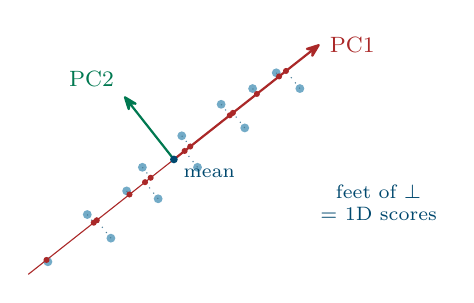
\begin{tikzpicture}[scale=1.0,>={Stealth[round]}]
  % PC1 line direction endpoints used for the perpendicular projection
  \coordinate (O) at (0,0);
  \coordinate (P1) at (1.85,1.46);
  % point cloud along a diagonal; foot = perpendicular projection onto PC1
  \foreach \x/\y in {-1.6/-1.3,-1.1/-0.7,-0.8/-1.0,-0.4/-0.1,-0.2/-0.5,
                     0.1/0.3,0.3/-0.1,0.6/0.7,0.9/0.4,1.3/1.1,
                     1.6/0.9,-0.6/-0.4,1.0/0.9}{
    \fill[tuwblue!55] (\x,\y) circle (1.6pt);
    \draw[dotted,tuwdark!70] (\x,\y) -- ($(O)!(\x,\y)!(P1)$);
    \fill[pitred] ($(O)!(\x,\y)!(P1)$) circle (1.1pt);}
  % PC1 (long axis, slope ~0.79) through the centroid (origin)
  \draw[->,thick,pitred] (0,0) -- (1.85,1.46) node[right]{\footnotesize PC1};
  \draw[pitred] (0,0) -- (-1.85,-1.46);
  % PC2 orthogonal
  \draw[->,thick,keygreen] (0,0) -- (-0.63,0.80) node[above left]{\footnotesize PC2};
  % centroid marker
  \fill[tuwdark] (0,0) circle (1.4pt) node[below right,font=\scriptsize]{mean};
  \node[tuwdark,font=\scriptsize,align=center] at (2.6,-0.55)
        {feet of $\perp$\\$=$ 1D scores};
\end{tikzpicture}
\end{center}
\sketchnote{Ellipse-shaped cloud; arrow PC1 along the long axis through the
centroid; short orthogonal arrow PC2; for each point a thin line dropped at a
right angle onto PC1; the feet of those perpendiculars are the 1D PCA scores.}
\end{exambox}

\begin{algobox}[MDS -- Multidimensional Scaling]
\textbf{Core idea:} find a low-dimensional embedding that \term{best preserves the
pairwise distances} $\delta_{i,j}$ of the high-dimensional data.\\
\textbf{Cost (stress):}
$\displaystyle \min_{\mathbf{x}_1,\dots,\mathbf{x}_n}\sum_{i<j}\bigl(\lVert
\mathbf{x}_i-\mathbf{x}_j\rVert-\delta_{i,j}\bigr)^2$.\\
\textbf{Variants:} \term{classical / metric} MDS preserves actual distance values
(classical MDS on Euclidean distances $\approx$ PCA); \term{non-metric} MDS
preserves only the \emph{rank order} of distances. Distances can be any metric
(e.g.\ cosine similarity for documents). \term{ISOMAP} $=$ MDS on \term{geodesic}
(manifold) distances instead of Euclidean -- a non-linear variant that unrolls
manifolds like the swiss roll.\\
\textbf{Properties:} preserves global distance structure; like PCA tends to keep
\emph{dissimilar} points far apart.\\
\textbf{Hyperparameters:} target dimension, metric, metric vs non-metric.\\
\textbf{Complexity:} works on the $n\times n$ distance matrix $\Rightarrow$
$O(n^2)$ memory/time, heavier for large $n$.\\
\textbf{When to use:} you have a meaningful (dis)similarity matrix and care about
preserving overall distances.\\
\textbf{Pitfalls:} struggles to keep \emph{very similar} points close (crowding);
$O(n^2)$ does not scale to huge $n$.
\end{algobox}

\begin{algobox}[t-SNE -- t-Distributed Stochastic Neighbor Embedding]
\textbf{Core idea:} preserve \term{local neighborhoods}, not distances. Model
high-dimensional similarities as conditional probabilities (Gaussian),
$p_{j|i}\propto\exp(-\lVert x_i-x_j\rVert^2/2\sigma_i^2)$, and low-dimensional
similarities with a heavy-tailed \term{Student-t} distribution $q_{j|i}$;
minimize the \term{Kullback--Leibler divergence}
$C=\sum_i \mathrm{KL}(P_i\Vert Q_i)$ by gradient descent.\\
\textbf{Key properties:} the Student-t tail solves the \term{crowding problem}
(room to spread out medium distances). Keeps similar points close;
\term{stochastic / non-deterministic} (different runs differ).\\
\textbf{Hyperparameters:} \term{perplexity} (effective \#neighbors defining the
Gaussian variance; balances local vs global, $\approx 5$--$50$), learning rate
($\epsilon$), iterations; can use Barnes--Hut approximation.\\
\textbf{Complexity:} heavier than PCA/UMAP; iterative optimization
($O(n^2)$ naive, $O(n\log n)$ with Barnes--Hut).\\
\textbf{When to use:} reveal local cluster structure (e.g.\ MNIST digit clusters).\\
\textbf{Pitfalls (heavily examined):} \emph{cluster sizes are NOT meaningful};
\emph{inter-cluster distances are NOT meaningful}; results depend on perplexity
and random seed; can show clusters in random data at low perplexity; preserves
no global geometry.
\end{algobox}

\begin{algobox}[UMAP -- Uniform Manifold Approximation and Projection]
\textbf{Core idea:} \term{manifold / graph-based}. Build a weighted
$k$-nearest-neighbor graph (a fuzzy topological / simplicial representation of the
manifold), then optimize a low-dimensional layout with the closest equivalent
fuzzy topological structure.\\
\textbf{Key properties:} like t-SNE preserves \term{local} neighborhoods but
tends to preserve \term{more global structure}; \term{faster} and scales better;
still \term{stochastic}.\\
\textbf{Hyperparameters:} \term{n\_neighbors} (size of local neighborhood from
which the manifold is learned -- larger $=$ more global view), \term{min\_dist}
(how tightly points may pack in the embedding -- smaller $=$ tighter clumps).\\
\textbf{Complexity:} approximate kNN $\Rightarrow$ scales to large $n$, faster
than t-SNE.\\
\textbf{When to use:} large datasets needing local \emph{and} some global
structure (single-cell, embeddings).\\
\textbf{Pitfalls:} absolute distances/densities still not fully reliable;
hyperparameter-dependent shapes; non-deterministic.
\end{algobox}

\begin{keybox}[Distortions \& the structure--interpretability trade-off]
Any DR projects feature space $\mathcal{D}$ to visual space $\mathcal{M}$ and
introduces \term{distortions}: \term{missing neighbors} (close in feature space
but far in the plot) and \term{false neighbors} (far in feature space but close
in the plot). Trade-off (Liu et al., 2017): \term{manifold learning} (t-SNE,
UMAP) captures the most intrinsic structure but has \emph{non-interpretable}
axes; \term{axis-aligned projection} (feature selection) has fully interpretable
axes but least structure; \term{linear projection} (PCA) sits in between.
Take-away: \emph{feature extraction leads to information loss}.
\end{keybox}

\subsubsection{Comparison Table: PCA vs MDS vs t-SNE vs UMAP}

\begin{center}
\begin{tabular}{@{}p{1.6cm}p{1.2cm}p{1.4cm}p{3.0cm}p{3.2cm}p{2.0cm}@{}}
\toprule
\textbf{Method} & \textbf{Linear?} & \textbf{Determ.?} & \textbf{Preserves}
& \textbf{Main hyperparameters} & \textbf{Scalability}\\
\midrule
\term{PCA}   & yes & yes & global variance / large distances; linear subspace
             & \#components $k$ & high ($O(d^3)$)\\
\term{MDS}   & no\textsuperscript{*} & yes (classical) & global pairwise distances
             (stress) & target dim; metric; (non)metric & low ($O(n^2)$)\\
\term{t-SNE} & no & \textbf{no} & local neighborhoods (cluster sizes \&
             inter-cluster dist.\ \emph{not} meaningful)
             & \textbf{perplexity}, learning rate $\epsilon$, iterations & medium\\
\term{UMAP}  & no & \textbf{no} & local $+$ more global structure (kNN graph /
             manifold) & \textbf{n\_neighbors}, \textbf{min\_dist} & high (fast)\\
\bottomrule
\end{tabular}
\end{center}
{\footnotesize\textsuperscript{*}Classical/metric MDS on Euclidean distances is
linear and coincides with PCA; non-metric MDS and ISOMAP are non-linear.}

\begin{exambox}[MCQ-style: properties \& hyperparameters]
\begin{itemize}
\item \emph{Which method is deterministic (same result every run)?} $\to$ PCA
      (and classical MDS). t-SNE and UMAP are \term{stochastic}.
\item \emph{Whose cluster sizes and inter-cluster distances are meaningless?}
      $\to$ \term{t-SNE} (and largely t-SNE-style layouts).
\item \emph{``Perplexity'' is a hyperparameter of \dots} $\to$ \term{t-SNE}
      (number of neighbors defining the Gaussian variance, balances local/global).
\item \emph{``n\_neighbors'' and ``min\_dist'' belong to \dots} $\to$ \term{UMAP}.
\item \emph{Which is the only linear method?} $\to$ \term{PCA} (and classical MDS).
\item \emph{PCA finds the directions of \dots} $\to$ \term{maximum variance} $=$
      eigenvectors of the covariance matrix; first PC $=$ largest eigenvalue.
\item \emph{Which best preserves global pairwise distances?} $\to$ MDS / PCA;
      \emph{which best preserves local neighborhoods?} $\to$ t-SNE / UMAP.
\end{itemize}
\end{exambox}

\begin{pitfall}[Over-interpreting a 2D projection]
Do not read meaning into t-SNE/UMAP \emph{distances}, cluster \emph{sizes}, or
empty gaps; do not call a t-SNE result reproducible; do not forget to
\emph{standardize} before PCA; remember that a low total explained variance means
the 2D PCA scatterplot is a weak summary. State that projection axes are
\emph{not interpretable} for feature-extraction methods.
\end{pitfall}

\section{Scalable Information Visualization \& Big Data}

\term{Big data} (Heer \& Kandel) has three dimensions: data can be \term{tall}
(billions/trillions of rows / items), \term{wide} (hundreds/thousands of
attributes / variables), and \term{diverse} (many sources, varied types). A
pragmatic visualization definition: \emph{big data = when our traditional
visual encodings break}. When each data record is mapped to one mark, naive
encodings (scatterplots, parallel coordinates) become unreadable already at
$10\,000$--$100\,000$ items.

\begin{keybox}[The exam-critical distinction: two kinds of scalability]
There are \textbf{two} separate scalability challenges. Naming both correctly
is the most common exam point.
\begin{itemize}
  \item \term{Perceptual scalability} --- can the user \emph{read} it?
        The display has fewer pixels than data points; too many marks cause
        \term{overplotting}, occlusion, clutter, low readability. Limited by
        \emph{human perception} (precision of the eye/mind) and \emph{display
        resolution}, not by the database. \emph{Goal: show a larger amount of
        data in a readable way} [Richer et al. 2022].
  \item \term{Interactive / computational scalability} --- is it \emph{fast}
        enough? Too much data to query/process at interactive rates:
        inefficient database queries, inefficient data processing,
        rendering-performance limits, interaction latency.
\end{itemize}
\textbf{Rule of thumb (latency):} the \term{100\,ms} interactive response-time
limit. Beyond it, exploration stalls. A Google study found that adding just
\term{200\,ms} latency to search measurably reduced the number of searches ---
and the effect persisted for weeks (Heer \& Kandel).
\end{keybox}

\subsection{Factors Affecting (Visual) Scalability}

\begin{keybox}[List: factors affecting scalability (Erick \& Karr 2012)]
\begin{tabular}{@{}ll@{}}
\toprule
Factor & Affects \\
\midrule
\term{Human perception} (precision of eye \& mind) & perceptual \\
\term{Monitor resolution} (physical size, \#pixels) & perceptual \\
\term{Visual metaphors} (choice of idiom \& channels) & perceptual \\
\term{Interactivity} (panning, zooming, brushing) & both \\
\term{Data structures \& algorithms} (graph layout, data cubes) & interactive \\
\term{Computational infrastructure} (CPU, GPU, network) & interactive \\
\bottomrule
\end{tabular}

\smallskip
The first three sit on the perceptual side; interactivity bridges; the last two
are the interactive/computational side. Also relevant: \#rows, \#dimensions,
memory.
\end{keybox}

\begin{keybox}[List: sources of latency (Heer \& Kandel)]
The interaction round-trip has three latency stages, each with its own fix:
\begin{enumerate}
  \item \term{Data query} --- searching too much data
        (e.g.\ \texttt{month=1} in 4\,M rows). \emph{Fix:} pre-computed
        aggregates / data cubes; plus data transfer (network) and disk I/O.
  \item \term{Data processing} --- aggregation/computation too slow.
        \emph{Fix:} parallelization (map-reduce style), prefetching.
  \item \term{Visualization / rendering} --- drawing too slow for
        interaction/animation (e.g.\ SVG/D3 does not scale with \#items).
        \emph{Fix:} bitmap/GPU rendering (WebGL, WebGPU) instead of SVG.
\end{enumerate}
\end{keybox}

\subsection{Overplotting: Simple Solutions vs.\ Preprocessing}

Each data record $\to$ one visual item. With big data this gives
\term{occlusion}, \term{clutter}, poor \term{readability}, and a
\term{waste of resources}.

\begin{keybox}[Simple solutions that need NO data preprocessing]
These touch only the \emph{rendering}, not the data:
\begin{itemize}
  \item \term{Alpha blending} (opacity/transparency) --- overlapping marks
        darken, revealing density. (Cannot show outliers + global patterns at
        once.)
  \item \term{Smaller marks} / reduced point size.
  \item \term{Jittering} --- small random offsets to separate coincident marks.
  \item \term{Draw order} (z-order) of marks.
  \item \term{Open vs filled} marks (outline-only marks occlude less).
\end{itemize}
\textbf{Contrast --- solutions that DO need preprocessing:} binning /
aggregation, sampling, kernel density estimation. The slides' ``3 simple
solutions'' are \term{alpha blending}, \term{filtering}, \term{random
sampling}; the warning: \emph{these cannot show global patterns and outliers at
the same time.}
\end{keybox}

\begin{pitfall}[Do not mix up the two solution classes]
Alpha blending, jittering, smaller/open marks, draw-order = \emph{no
preprocessing}. Binning, aggregation, density estimation, sampling =
\emph{preprocessing}. If asked for ``simple solutions to overplotting that need
no preprocessing'', listing binning loses the point.
\end{pitfall}

\subsection{Aggregation \& Density: Scalable Encodings}

Core idea: \emph{visualize \textbf{models} or \textbf{aggregates} of attributes
instead of individual data points} --- individual items are combined. The
perceptual scalability of a display should be limited by the chosen
\emph{resolution of the data}, not by the number of records (Heer \& Kandel).

\begin{algobox}[Binning / 2D histograms]
\textbf{Idea:} split the data range into regular \term{intervals (bins)};
encode the \term{frequency} (count per bin). Quantitative/ordinal $\to$ regular
intervals; nominal/categorical $\to$ one bin per category.\\
\textbf{Scalable because} we control the \emph{number of bins} independently of
\#records; same visual encoding as a bar chart (length/position).\\
\textbf{Hyperparameter:} bin size / number of bins.\\
\textbf{Pitfall:} sensitive to bin size --- can cause \term{aliasing} effects
(e.g.\ 9 vs 10 bins, $10\times10$ vs $30\times30$ bins look very different).
\end{algobox}

\begin{algobox}[Hexagonal binning (hexbin)]
2D binning where bins are \term{hexagons} instead of squares.\\
\textbf{Why hexagons:}
\begin{itemize}
  \item \term{Nearest-neighbour symmetry} --- all 6 neighbours are at the
        \emph{same distance} (a square grid mixes edge- and corner-neighbours,
        introducing visual bias).
  \item Hexagons are the \emph{maximum-side regular polygon that tessellates}
        the plane $\to$ most ``circular'', efficient density approximation.
\end{itemize}
Frequency encoded by \emph{colour or size}. \textbf{Hyperparameter:} bin size /
number of bins. Used in hexbin scatterplots, hexbin SPLOMs (Carr et al.\ 1987),
and geographic hexbin maps (e.g.\ Walmart / farmers' markets in the U.S.).
\end{algobox}

\begin{algobox}[Kernel Density Estimation (KDE)]
\textbf{Non-parametric} estimate of the probability density function of a
random variable by weighting distances of observations $x_1,\dots,x_n$ from a
query point $x$:
\[
  \widehat{f}_h(x) \;=\; \frac{1}{n}\sum_{i=1}^{n} K_h\!\left(x - x_i\right).
\]
\textbf{Hyperparameters:}
\begin{itemize}
  \item \term{Bandwidth} $h$ (kernel width): the larger $h$, the
        \emph{smoother} the curve.
        \emph{Too small} $\to$ \term{under-smoothing} (noisy, spiky);
        \emph{too large} $\to$ \term{over-smoothing} (a single blob; range and
        mode become misleading).
  \item \term{Kernel} $K$: non-negative, integrates to 1, mean 0 ---
        usually a \emph{Gaussian} (a rectangular/box kernel also works).
\end{itemize}
\textbf{Used in:} violin plots (density + embedded box plot, good for
\term{multimodal} distributions), density scatterplots (2D KDE), geographic
heatmaps. Munzner's \emph{continuous scatterplots} use the same idea: a derived
\emph{overplot-density} value coloured per pixel instead of discrete dots.
\end{algobox}

\begin{algobox}[Sampling (random / stratified)]
Show a \emph{representative subset} with a bounded number of points instead of
all records.\\
\textbf{Random sampling:} simple, uniform; risks dropping rare outliers.\\
\textbf{Stratified sampling:} sample within groups/strata so each is
represented --- better coverage of minority categories.\\
\textbf{Trade-off:} fewer marks $\to$ less overplotting and faster rendering,
but \emph{outliers and fine structure can be lost}. Can be combined with
aggregation (aggregate views of well-chosen samples approximate the full data).
\end{algobox}

\subsection{Data Cubes / Multi-Dimensional Tables (OLAP)}

For \emph{interactive} scalability, the killer technique is to
\term{pre-aggregate whatever possible} so that interactive queries hit small
precomputed tables, not the raw rows.

\begin{algobox}[Data cubes / multi-dimensional tables]
\textbf{From flat to cube:} a flat table (1 key $\to$ list, 2 keys $\to$
matrix/contingency table) generalizes to an $n$-dimensional \term{data cube}.
Each \emph{cell stores a precomputed aggregate} (\textbf{sum}, mean, count,
min/max).\\
\textbf{OLAP operations:}
\begin{itemize}
  \item \term{Roll-up} (projection): aggregate away a dimension
        (e.g.\ project onto $(\text{Time},\text{Products},*)$).
  \item \term{Drill-down}: the inverse --- go to a finer level of detail.
  \item \term{Slice}: fix one dimension to a single value (e.g.\ Texas).
  \item \term{Dice}: select a sub-range on several dimensions.
\end{itemize}
\textbf{Why it enables interactive scalability:} brushing/linking, dynamic
queries, panning/zooming become lookups + small re-aggregations over the cube
$\to$ within the 100\,ms budget.\\
\textbf{Cost (key pitfall):} size of the cube $=\prod_i b_i$ (product of bin
counts per dimension) --- \term{exponential in the number of dimensions}. So
pre-compute \emph{wisely} (only frequent / low-order projections; supports
simple, not arbitrary compound and/or queries).
\end{algobox}

\begin{keybox}[imMens / Nanocubes idea]
\term{imMens} [Liu, Jiang \& Heer 2013] and \term{Nanocubes} [Lins et al.\
2013]: precompute \term{binned aggregates} (multivariate data tiles) so that
\term{real-time brushing \& linking} over hundreds of millions of records stays
interactive (e.g.\ Brightkite $\sim$4\,M check-ins: brush ``January'' in a month
histogram $\to$ map + day + hour views update instantly). Brushing/linking =
filter + new aggregation; panning/zooming = change of bin resolution / \#samples.
\end{keybox}

\subsection{Reducing Processing \& Rendering Latency}

\begin{keybox}[Techniques (Heer \& Kandel; slides)]
\begin{itemize}
  \item \term{Parallel aggregation} / data-parallel processing (map-reduce
        style, GPU/clusters). Requirements: data must be \term{separable} (can
        be split and re-composed, e.g.\ local histograms merged into a global
        one) and \term{streamable} (processed independently). Tools: Dask,
        RAPIDS, PySpark.
  \item \term{Prefetching} \& \term{predictive caching} --- fetch data tiles
        the user is likely to request next (e.g.\ adjacent zoom levels).
  \item \term{Progressive / online aggregation \& sampling} --- show an
        approximate result immediately and refine it, so the user is never
        blocked waiting for the exact answer.
  \item \term{GPU / bitmap rendering} (WebGL, WebGPU) instead of SVG (D3),
        which does not scale with \#items.
\end{itemize}
\end{keybox}

\subsection{Reduce Strategy (Munzner ch.\ 13)}

\begin{keybox}[Filter vs Aggregate vs Embed]
\term{Reduce} is one of Munzner's strategies for managing complexity. It applies
to both \emph{items} and \emph{attributes} (= ``elements'').
\begin{itemize}
  \item \term{Filter} --- simply \emph{eliminate} elements (item filtering /
        attribute filtering), often via \term{dynamic queries}
        (tightly-coupled encoding $+$ interaction; e.g.\ FilmFinder, scented
        widgets). \emph{Risk:} ``out of sight, out of mind'' --- users forget
        filtered-out data.
  \item \term{Aggregate} --- replace a group of elements by a single
        \emph{derived} element that stands in for them (count, sum, mean,
        min/max). Cognitively safer (conveys info about the whole group) but
        \emph{cannot convey everything omitted}; the challenge is summarizing
        without hiding signal (cf.\ Anscombe's quartet). Examples: histograms,
        continuous scatterplots, box plots.
  \item \term{Embed} --- show focus and context together in one view
        (focus+context), so detail and overview coexist without removing data.
\end{itemize}
\end{keybox}

\subsection{Interactive Exploration: Shneiderman's Mantra}

\term{Overview first, zoom and filter, details on demand} [Shneiderman 1996]
maps directly onto scalable techniques:
\begin{itemize}
  \item \term{Overview} via aggregate visualizations (binned/hexbin maps,
        heatmaps, choropleths).
  \item \term{Zoom} via \term{hierarchical aggregation} / \term{semantic
        zooming} (drill-down): objects change shape/detail and new objects
        appear --- not just resizing. Aggregate visualizations are very well
        suited to this.
  \item \term{Filter} via \term{brushing \& linking} / dynamic queries.
  \item \term{Details on demand}: tooltips that report \emph{summary statistics
        of the aggregate / bin} (e.g.\ a hexbin tooltip: \#users, \#posts,
        \#locations in that bin).
\end{itemize}

\begin{exambox}[Worked connection: 10M traffic accidents]
\textbf{Task:} explore $\sim$10\,M traffic-accident records (location, time,
severity) interactively. Both scalability challenges appear --- name and solve
each:
\begin{description}
  \item[Perceptual scalability] 10\,M point marks on a map $\to$ total
        overplotting. \emph{Solution:} \term{aggregate}. Bin
        \emph{spatially} (regions/states, or a hexbin grid) and
        \emph{temporally} (by year). Encode counts by colour $\to$
        \term{choropleth} or \term{hexbin density map} (space) and a
        \term{line chart} of accidents per year or a \term{histogram} per
        region (time).
  \item[Interactive scalability] Re-querying 10\,M rows on every brush exceeds
        100\,ms. \emph{Solution:} build a \term{data cube} over
        $(\text{region}\times\text{year}\times\text{severity})$ with
        precomputed counts; brushing/linking then becomes cube lookups +
        small re-aggregations. Cost $\prod_i b_i$ stays small because only a
        few coarse dimensions are binned.
  \item[Linked views] A \term{choropleth/hexbin map} linked to a
        \term{line chart / histogram}: brush a year on the line chart $\to$ map
        re-aggregates; brush a region $\to$ time chart updates. Add
        details-on-demand tooltips reporting per-bin summary stats. If still
        slow: parallel aggregation + prefetching + progressive refinement.
\end{description}
\textbf{One-liner answer:} \emph{bin spatially \& temporally for perceptual
scalability; data cube for interactive scalability; linked
choropleth/hexbin map $+$ line chart.}
\end{exambox}

\begin{exambox}[How this is asked]
\begin{itemize}
  \item ``Name and distinguish the two scalability challenges'' $\to$
        perceptual vs interactive/computational (see top keybox).
  \item ``List factors affecting scalability'' / ``list sources of latency''
        $\to$ the two list-keyboxes above; map each to perceptual/interactive.
  \item ``Give simple overplotting solutions needing no preprocessing'' $\to$
        alpha, smaller/open marks, jitter, draw-order (NOT binning/sampling).
  \item ``Why hexagons?'' $\to$ uniform neighbour distance + best regular
        tessellation.
  \item ``KDE bandwidth too large/small?'' $\to$ over-/under-smoothing.
  \item ``Why are data cubes expensive?'' $\to$ size $\prod_i b_i$, exponential
        in \#dimensions.
  \item ``Munzner reduce'' $\to$ filter vs aggregate vs embed.
\end{itemize}
\end{exambox}

\section{Network and Tree Visualization}

This is a high-priority exam topic: graph-drawing algorithms appear under
``Visualization Algorithms'', and node-link\,$\leftrightarrow$\,matrix and
treemap\,$\leftrightarrow$\,node-link tree appear under ``Mapping data items'' /
``Alternatives''. The aesthetic-criteria list and the force-directed / layered /
morphing / foresighted layouts are recurring question targets.

\subsection{Graph basics}

\begin{keybox}[Definitions]
A \term{graph} $G=(V,E)$ is an abstract structure for modelling
\emph{relational} information: $V$ is a set of \term{nodes} (objects), $E$ a set
of \term{edges} (relations connecting nodes).
\begin{itemize}
  \item \term{Directed} vs.\ \term{undirected}: edges may have a direction. In a
  directed graph the \term{in-degree} of a node is the number of incoming edges,
  the \term{out-degree} the number of outgoing edges. The \term{degree} is the
  number of incident edges.
  \item \term{Weighted}: edges (or nodes) can carry \term{values} (edge weights),
  possibly of different types.
  \item Graphs may contain \term{cycles}; special families: planar, bipartite,
  hierarchical, clustered graphs, and \term{hypergraphs} (an edge connects more
  than two nodes).
  \item \term{Tree} = special case of a graph: \emph{no cycles}, one special
  \term{root} node, every non-root node has exactly one parent. Variants: free,
  binary, rooted, ordered trees.
  \item \term{Network} = graph + attributes on nodes/edges. A
  \term{multivariate network} attaches many attributes per element (primary data:
  directly measured; secondary data: derived/computed).
\end{itemize}
\end{keybox}

\paragraph{Data structures and the two visual representations.}
Internally a graph is stored as an \term{adjacency matrix} ($|V|\times|V|$, entry
$=1$ / weight if edge present) or an \term{adjacency list}. For \emph{display}
there are two fundamental mappings of the same data:

\begin{center}
\begin{minipage}{0.42\linewidth}\centering
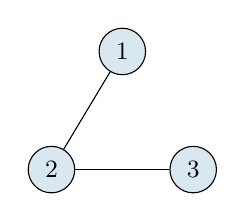
\begin{tikzpicture}[every node/.style={font=\small}]
  \node[circle,draw,fill=tuwblue!15] (a) at (0,1.5) {1};
  \node[circle,draw,fill=tuwblue!15] (b) at (-0.9,0) {2};
  \node[circle,draw,fill=tuwblue!15] (c) at (0.9,0) {3};
  \draw (a)--(b); \draw (b)--(c);
\end{tikzpicture}\\[2pt]
{\small Node--link diagram}
\end{minipage}\hfill
\begin{minipage}{0.42\linewidth}\centering
\begin{tabular}{c|ccc}
  & 1 & 2 & 3 \\ \hline
1 & 0 & 1 & 0 \\
2 & 1 & 0 & 1 \\
3 & 0 & 1 & 0 \\
\end{tabular}\\[4pt]
{\small Adjacency matrix}
\end{minipage}
\end{center}

\subsection{Node-link vs.\ adjacency matrix (mapping \& alternatives)}

The two are the classic \term{alternative representations} of the \emph{same}
relational data, with complementary strengths.

\begin{center}
\begin{tabular}{p{0.30\linewidth} p{0.31\linewidth} p{0.31\linewidth}}
\toprule
 & \term{Node--link} & \term{Adjacency matrix} \\
\midrule
Edge $\to$ visual mark & line/curve between two node marks & filled cell
$(i,j)$ (colour/size $\to$ weight) \\
Path following / topology & \textbf{good} -- follow lines, see connectivity,
clusters by spatial proximity & \textbf{hard} -- must hop row$\to$column
mentally; multi-hop paths very tedious \\
Density / scalability & degrades on \textbf{dense} graphs (hairball, many edge
crossings, occlusion) & \textbf{good} on dense graphs: \emph{no edge crossings},
no overlap, every edge visible \\
Clusters / cliques & visible if layout separates them & a clique = solid block
on the diagonal; easy to spot with good row/column ordering \\
Space & compact for \emph{sparse} graphs & always $|V|^2$ cells \\
\bottomrule
\end{tabular}
\end{center}

\begin{keybox}[One-line rule of thumb]
\emph{Sparse} graph + need to \emph{follow paths / read topology} $\Rightarrow$
\term{node--link}. \emph{Dense} graph + want to spot \emph{clusters/cliques} and
avoid crossings $\Rightarrow$ \term{matrix}. Hybrid \term{NodeTrix} (Henry et
al.\ 2007) draws dense communities as small matrices and the sparse links
between them as node--link edges.
\end{keybox}

\subsection{Aesthetic criteria for graph drawing (the ``List'' topic)}

A good layout should be \emph{easy to read, understand and remember}. Layout
algorithms try to satisfy a set of \term{aesthetic criteria}; these are often
\emph{contradictory} and their optimisation is mostly \emph{NP-hard}, so most
graph-drawing algorithms are \term{heuristics}.

\begin{keybox}[Aesthetic criteria -- memorise the list]
\begin{itemize}[leftmargin=1.4em]
  \item Minimise \term{edge crossings} $\downarrow$
  \item Minimise \term{bends} of edges $\downarrow$ (max / uniform / total bends)
  \item Maximise \term{symmetry} $\uparrow$
  \item \term{Edge length} $\downarrow$: short, and \emph{uniform} edge lengths
  \item Even \term{node distribution}; \term{avoid node overlap}
  \item Minimise drawing \term{area} $\downarrow$
  \item Maximise \term{angular resolution} (``resolution'' $\uparrow$): angles
  between edges at a node should be large
  \item Show \term{clusters} / community structure
\end{itemize}
\end{keybox}

\begin{pitfall}[Criteria conflict]
The criteria \emph{trade off}. Classic exam example: a $K_4$ drawn as a
\emph{triangle with a centre node} has \emph{zero crossings} but no symmetry;
drawn as a \emph{square with both diagonals} it is fully \emph{symmetric} but has
one crossing. You cannot maximise everything at once -- say so explicitly.
\end{pitfall}

\subsection{Layout algorithm: Force-directed / spring embedder}

\begin{algobox}[Force-directed (spring embedder, Eades 1984)]
\textbf{Idea.} Model the graph as a \emph{physical system}: edges act as
\term{springs} (attractive force pulling adjacent nodes together, $\sim$ spring
toward a rest length), and \emph{all} pairs of nodes exert a \term{repulsive}
force (like charges / ``gravitation between nodes''). Iterate: compute net force
on each node, move it a little, repeat until the system reaches a
\term{stable, low-energy configuration} (energy minimisation).\\[2pt]
\textbf{Properties.} Produces \emph{symmetric, organic} layouts with
\emph{uniform edge lengths} -- exactly the two criteria Eades targeted. Works
well on small/medium sparse graphs; reveals clusters. Generalises to 3D.\\[2pt]
\textbf{Hyperparameters.} Spring constant / ideal (rest) edge length, repulsion
strength, step size or \term{temperature} (cooling schedule, as in
Fruchterman--Reingold), number of \term{iterations}, initial (often random)
placement.\\[2pt]
\textbf{Complexity.} Naive: $O(n^2)$ repulsion per iteration (all node pairs)
$\times$ iterations. \term{Barnes--Hut} approximation groups distant nodes into a
quad/oct-tree and treats each group as one pseudo-node $\Rightarrow$
$O(n\log n)$ per iteration.\\[2pt]
\textbf{Pitfalls.} \emph{Non-deterministic} (depends on random start);
gets stuck in \emph{local minima}; classic spring embedder has \emph{high
runtime} and can \emph{break down on very large graphs}. Improvements:
Kamada--Kawai 1989 (local minimal energies), Fruchterman--Reingold 1991, Davidson
\& Harel 1996 (simulated annealing).
\end{algobox}

\subsection{Layout algorithm: Layered / Sugiyama (hierarchies, flow)}

\begin{algobox}[Layered graph drawing (Sugiyama--Tagawa--Toda 1981)]
\textbf{Idea.} For \emph{directed} graphs / DAGs, hierarchies, and flow: arrange
nodes in horizontal \emph{layers} (rows) so all edges point downward. Classic
pipeline:
\begin{enumerate}[leftmargin=1.5em]
  \item \term{Cycle removal} -- extract an acyclic subgraph that contains all
  nodes (temporarily reverse a few edges).
  \item \term{Layer assignment} -- give each node an integer layer number; nodes
  arranged top-down in rows. (Long edges get \emph{dummy nodes} on intermediate
  layers.)
  \item \term{Crossing minimisation} -- choose the \emph{order} within each row to
  reduce edge crossings, typically layer-by-layer (e.g.\ \term{barycenter}
  heuristic: put a node at the average position of its neighbours in the adjacent
  layer).
  \item \term{Coordinate assignment} -- assign final $x$/$y$ to straighten edges
  and balance spacing.
\end{enumerate}
\textbf{Properties.} Emphasises \emph{direction / hierarchy / flow}; good for
DAGs, dependency and process diagrams. Variants: \emph{parallel layers}
(top-down rows) and \emph{radial layers} (concentric rings). \\[2pt]
\textbf{Hyperparameters.} Layer-assignment policy (longest-path, network-simplex),
crossing-minimisation heuristic and \#sweeps, node/layer spacing. \\[2pt]
\textbf{Complexity.} Even 2-layer crossing minimisation is \emph{NP-hard}
$\Rightarrow$ heuristics (barycenter, median). \\[2pt]
\textbf{Pitfalls.} Cycles must be handled first; dummy nodes inflate the graph;
poor for undirected / non-hierarchical graphs.
\end{algobox}

\subsection{Dynamic graphs and the mental map}

Networks increasingly \emph{change over time} (biochemical pathways gain new
reactions, social contacts appear/disappear). Visualisations of such dynamic
graphs must \term{preserve the ``Mental Map''} (Misue, Eades, Lai, Sugiyama
1995): the user should \emph{recognise old structures again} across time steps,
so nodes should not jump around between frames.

\begin{algobox}[Graph morphing]
\textbf{Idea.} Visualise the transition between two layouts with \emph{smooth
animation}: if a node changes position, compute an \emph{interpolated animation
path} between old and new position. Can be applied on top of \emph{any} 2D/3D
layout algorithm (e.g.\ GraphAEL uses force-based layouts).\\
\textbf{+} Looks good, eases tracking. \textbf{--} Nodes \emph{still change
position}; newly added or deleted nodes may not be correctly identified. This is
an \term{online} approach: lay out each step, then animate between consecutive
steps.
\end{algobox}

\begin{algobox}[Foresighted layout (Diehl, G\"org, Kerren 2001)]
\textbf{Idea.} If the \emph{whole sequence} of graphs is known (or can be
pre-computed) -- an \term{offline} setting -- build a \term{supergraph} (union of
all time steps) and compute \emph{one} layout from it. Position nodes at the
start so that they \emph{do not change their positions later} across the whole
sequence.\\
\textbf{+} \emph{Best mental-map preservation}; \emph{independent} of the chosen
layout algorithm. \textbf{--} The sequence is \emph{often unknown} in advance;
partly poor aesthetics (e.g.\ gaps at the beginning where future-only nodes are
reserved).
\end{algobox}

\begin{keybox}[Online vs.\ offline; animation vs.\ juxtaposition]
\term{Online}: layout per step as data arrives (morphing animates between them).
\term{Offline}: full sequence known $\Rightarrow$ foresighted layout for stable
positions. Time can be shown by \term{animation} (one view, moving) or by
\term{small multiples / timeline} (many static views side by side, e.g.\
\emph{matrix cubes}: stack adjacency matrices into a space-time cube).
\end{keybox}

\subsection{Tree layouts}

\begin{keybox}[Tree drawing families]
\begin{itemize}
  \item \term{Node--link trees}: \term{rectilinear} (classic top-down/left-right
  hierarchy with root on top) or \term{radial} (root in centre, depth $\to$
  radius).
  \item \term{Indented / outline} layout: nested indentation (like a file
  explorer); depth $\to$ horizontal indent.
  \item \term{Space-filling treemap}: \emph{recursive subdivision} of a rectangle.
  Hierarchy is encoded by \term{containment} (child rectangles nested inside the
  parent); a \emph{leaf}'s value is mapped to its \term{area}. No wasted
  whitespace. Algorithms: \term{slice-and-dice} (alternate cut direction per
  level -- simple but produces thin slivers) vs.\ \term{squarified} (keep cells
  close to square -- better aspect ratio, easier area comparison).
\end{itemize}
\end{keybox}

\begin{exambox}[Mapping data items: treemap $\leftrightarrow$ node-link tree]
\term{Treemap} and \term{rectilinear node-link tree} are two encodings of the
\emph{same hierarchy}. Node--link shows \emph{structure/depth} explicitly but
wastes space and scales poorly; treemap is \emph{space-filling} and great for
comparing \emph{leaf values by area} but makes the \emph{topology/depth} hard to
read. Containment (treemap) vs.\ connection (node--link) is the underlying
encoding difference.
\end{exambox}

\subsection{Biological networks (Kerren)}

Modern \term{systems biology} treats biological processes as integrated systems
of many interacting components; high-throughput methods (since the human genome
project) produce huge data, and \term{networks are the key concept} to structure
and combine it.

\begin{keybox}[Types of biological networks (a hierarchy)]
\begin{itemize}
  \item \term{Molecular graphs} -- atoms/bonds of a single molecule.
  \item \term{Metabolic networks / pathways} -- nodes are substances, edges are
  reactions, each single reaction catalysed by an \term{enzyme}; a \term{pathway}
  is a sequence of reactions converting one substance into another (databases:
  \emph{KEGG}; tools: PathViewer, BioPath, VANTED).
  \item \term{Protein--protein interaction (PPI) networks} -- nodes are proteins,
  edges are interactions (e.g.\ \emph{signal transduction}); fundamental for many
  functions and diseases (tool: \emph{Cytoscape}).
  \item \term{Gene regulatory networks} -- regulatory relations between genes.
\end{itemize}
Why it matters: diseases interpreted in a network context (infection = a foreign
network operating in ours; genetic defect = incorrect connectivity);
applications in drug design and metabolic engineering.
\end{keybox}

\begin{keybox}[Challenges \& integrative bioinformatics]
\textbf{Challenges:} \emph{scale} (huge networks, scalability/navigation);
\emph{integrating multiple heterogeneous data types} onto network elements
(multivariate primary/secondary attributes); respecting \emph{standard pathway-map
conventions} (e.g.\ KEGG layouts biologists expect).\\
\textbf{Integrative bioinformatics} combines network topology with the attached
multivariate data. State-of-the-art strategies (cf.\ the multivariate-network
slides):
\begin{itemize}
  \item \term{Integrated approaches} -- replace nodes by embedded diagrams
  (e.g.\ bar charts in pathway nodes).
  \item \term{Multiple coordinated views} -- network view linked with parallel
  coordinates, heatmaps, etc.\ (brushing-and-linking; e.g.\ Caleydo).
  \item \term{Semantic substrates} -- node position fixed by attributes in
  non-overlapping regions; edge slider controls clutter.
  \item \term{Attribute-driven topology} / hybrid (JauntyNets) -- user balances
  whether \emph{topology} or \emph{attributes} drive the force layout.
\end{itemize}
\end{keybox}

\subsection{Exam boxes}

\begin{exambox}[MCQ: node-link vs.\ adjacency matrix]
\emph{``For a large, very dense network where the analyst wants to find tightly
connected communities, which representation is preferable, and why?''} \\
Answer: the \term{adjacency matrix}. On dense graphs node--link becomes a
hairball with many crossings/occlusion, whereas a matrix has \emph{no edge
crossings}, shows \emph{every} edge, and -- with good row/column ordering --
makes cliques appear as solid diagonal blocks. Trade-off: \emph{path following}
across multiple hops is much harder in a matrix, so for sparse graphs / topology
tracing, prefer \term{node--link}.
\end{exambox}

\begin{exambox}[MCQ: force-directed vs.\ layered]
\emph{Which layout for an undirected social network where symmetry and uniform
edge length matter?} $\Rightarrow$ \term{force-directed}. \emph{Which for a
directed DAG / dependency or process flow?} $\Rightarrow$ \term{layered /
Sugiyama}. Distractor traps: force-directed is \emph{non-deterministic} and prone
to \emph{local minima} (true); Sugiyama's crossing minimisation is
\emph{NP-hard} hence heuristic (true); force-directed is naively $O(n^2)$ per
iteration, reducible to $O(n\log n)$ via \term{Barnes--Hut} (true).
\end{exambox}

\begin{exambox}[MCQ: morphing vs.\ foresighted layout]
Both aim to \term{preserve the mental map} of a \emph{dynamic} graph.
\term{Morphing} = \emph{online}, animate (interpolate) between per-step layouts;
nodes still move, can be applied to any layout, but added/removed nodes are hard
to follow. \term{Foresighted layout} = \emph{offline}, needs the full sequence,
computes a \emph{supergraph} so node positions \emph{stay stable} across all time
steps; best mental-map preservation but sequence often unknown and aesthetics can
suffer (gaps). Common wrong answer: claiming foresighted works online -- it does
\emph{not}; it requires the sequence in advance.
\end{exambox}

\section{Complex Data: Sets, Curves, and Ensembles}

Classic multidimensional data has records with numerical and categorical
attributes. \term{Complex data} adds richer attribute kinds: \term{sets},
\term{curves} (function graphs / time series), and \term{surfaces}. This
section covers three such cases that recur in the exam: set-typed data
(how to visualise it, with UpSet as the modern go-to answer), families of
function graphs (Konyha et al.), and simulation ensembles (Matkovic et al.).
All three are united by one idea: an attribute is no longer a single scalar
but a structured object, and the same visual-analysis toolkit
(\term{coordinated multiple views} + \term{brushing and linking}) is used to
explore them.

% ======================================================================
\subsection{Set-Typed Data}

\begin{keybox}[Definition]
\term{Set-typed data}: a collection of \term{elements}, each of which has a
membership in one or more of several \emph{possibly overlapping} \term{sets}.
Equivalently, each element carries a \term{set-typed attribute} whose value is
a subset of the universe of sets (a \term{set family} / set system over the
elements). Sets may relate by \term{containment, exclusion, and intersection}.
\end{keybox}

\textbf{Example (movies).} Universe of sets $=$ genres
$\{\text{Romance},\text{Drama},\text{Comedy},\dots\}$. Each movie is an element;
its set-typed attribute is its genre set, e.g.
\textit{Cinema Paradiso} $=\{$Romance, Drama, Comedy$\}$, \textit{Touch}
$=\{$Romance$\}$. Other real-world cases: club memberships, product features,
employee skill sets, search-engine result overlaps, patient symptoms.

\textbf{Key notions} (Sets-STAR, Alsallakh et al.).
\begin{itemize}
\item \term{Set membership degree} of an element $=$ number of sets it
  belongs to (its \term{degree}).
\item \term{Exclusive membership}: an element belongs to exactly one set / one
  specific intersection.
\item \term{Intersection / overlap}: the set of elements shared by a group of
  sets. With $n$ sets there are up to $2^n$ possible membership combinations,
  which is why naive approaches do not scale.
\item Data representations: cardinalities only, multi-valued attribute
  (adjacency-list style), membership lists (edge-list style), or Boolean
  attributes (adjacency-matrix style).
\end{itemize}

\textbf{Typical tasks} (what a technique must support): find elements of a set,
find sets of an element, filter by membership degree; find the number of sets;
analyse inclusion / exclusion / intersection relations; identify the sets in a
given intersection and the largest / smallest intersections; compare set and
intersection cardinalities and similarities.

\subsubsection{Techniques (Sets-STAR categories)}

\begin{algobox}[Euler / Venn diagrams]
\textbf{Idea:} sets $=$ labelled closed curves (circles, ellipses, polygons);
set relations $=$ curve overlaps. A \term{Venn} diagram shows \emph{all} $2^n$
possible overlaps; an \term{Euler} diagram shows only the overlaps that
actually occur (it can be \term{well-matched}: regions reflect the true
relations).\\
\textbf{Reads:} membership pops out preattentively via enclosure.\\
\textbf{Trade-offs:} \emph{does not scale beyond $\sim$3 sets}; for $\ge 4$
sets, well-matched + well-formed (simple, smooth, area-proportional) curves are
often impossible, and \emph{some intersections become undrawable}. Area-judgement
bias hurts area-proportional variants.
\end{algobox}

\begin{algobox}[Over-plotting / point-based (overlays)]
\textbf{Idea:} elements live in an existing layout (scatterplot, map, graph)
and set membership is overlaid with \term{colour/glyphs} (coloured dots,
pie-glyphs, hatching) or with \term{region} overlays (\term{Bubble Sets},
texture splatting) or \term{line} overlays (\term{LineSets}, \term{Kelp
Diagrams}).\\
\textbf{Use when:} elements have a meaningful spatial reference and set
membership is secondary. Region overlays handle $\sim$4--20 sets.\\
\textbf{Trade-offs:} limited number of sets/elements; layout artifacts
(spurious overlaps, crossings); overlays cannot move the elements.
\end{algobox}

\begin{algobox}[Matrix-based]
\textbf{Idea:} a \term{set-membership matrix} -- rows $=$ elements, columns $=$
sets (cells mark membership); or sets $\times$ sets cells holding a similarity /
overlap measure (heatmap). Reordering rows/columns reveals clusters of similar
membership. Examples: ConSet, PixelLayers, frequency grids.\\
\textbf{Trade-offs:} fairly scalable in both elements and sets, clutter-free
(no edge crossings), but limited in which set \emph{relations} they express,
and patterns are \emph{sensitive to ordering}.
\end{algobox}

\begin{algobox}[Node-link / graph-based]
\textbf{Idea:} model element--set membership as a \term{bipartite graph} (edges
$=$ memberships). Examples: Jigsaw lists, anchored maps, PivotPaths; Radial
Sets / Circos for set--set links.\\
\textbf{Trade-offs:} elements are visible as individual objects and clusters of
similar membership show up, but \emph{limited scalability due to edge
crossings}; element--set diagrams show no set relations directly.
\end{algobox}

\begin{algobox}[Aggregation-based]
\textbf{Idea:} when elements are many, follow ``overview first'': aggregate
elements into a single visual element encoding a \emph{frequency}. Bar charts of
set/intersection sizes, \term{Set'o'gram} (Freiler et al.), Mosaic / Double-Decker
plots, Parallel Sets, \term{Radial Sets} (Alsallakh et al.).\\
\textbf{Trade-offs:} \emph{highly scalable in number of elements}; some show how
attributes correlate with membership; but usually do not show single elements
as objects and are limited in set relations.
\end{algobox}

\begin{keybox}[UpSet -- the modern go-to technique]
Lex, Gehlenborg, Strobelt, Vuillemot \& Pfister, \emph{UpSet: Visualization of
Intersecting Sets}, IEEE TVCG 2014. \textbf{This is the standard answer to
``how do you visualise set-typed data with many sets?''}
\end{keybox}

UpSet replaces the overlapping regions of an Euler/Venn diagram with a
\term{matrix of intersections} plus \term{bar charts}:
\begin{itemize}
\item \textbf{Set-size bars} -- one bar per set giving each set's cardinality.
\item \textbf{Intersection matrix} -- columns are the (non-empty) intersections;
  each column is a vertical strip of dots over the set rows. A \term{filled
  dot} $=$ ``in this set'', an \term{empty dot} $=$ ``not in this set''; dots in
  the same column are joined by a line. A column with one filled dot $=$
  ``only in that set''; all dots filled $=$ ``in all sets''.
\item \textbf{Intersection-size bars} -- a bar chart giving the cardinality of
  each intersection, usually \emph{sorted} (e.g. by size) so the dominant
  combinations are obvious.
\end{itemize}
Because intersections are laid out as a sortable list rather than packed into
the plane, UpSet \emph{scales to many sets and many elements} and makes the
hard set tasks (which sets are in an intersection? which intersection is
largest?) directly readable. Related slide techniques: OnSet (binary
set matrices with set operations), Radial Sets, Set'o'gram.

\begin{pitfall}[Common deductions]
Do not draw a Venn diagram for $\ge 4$ sets and claim it ``works'' -- some
intersections are undrawable and area judgements are biased. Do not show set
sizes as a \term{pie chart}: set categories are not mutually exclusive and do
not sum to a whole. For ``many sets'' always reach for \textbf{UpSet} (or
aggregation/matrix methods), not Euler/Venn.
\end{pitfall}

\begin{center}
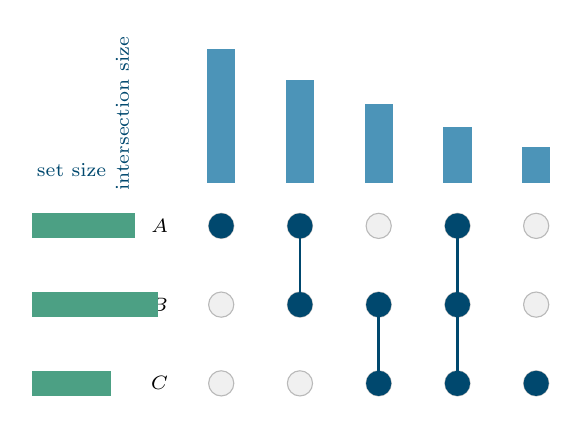
\begin{tikzpicture}[x=1cm,y=1cm,font=\scriptsize]
  % --- geometry: matrix rows A,B,C at y=2,1,0 ; columns x=0..4 ---
  \def\rA{2} \def\rB{1} \def\rC{0}
  % intersection-size bars (top), sorted descending
  % columns and the heights of their size bars
  \foreach \x/\h in {0/1.7,1/1.3,2/1.0,3/0.7,4/0.45}{
    \fill[tuwblue!70] (\x-0.18,2.55) rectangle (\x+0.18,{2.55+\h});}
  \node[anchor=south,rotate=90,tuwdark] at (-1.05,3.4)
        {\,intersection size};
  % --- matrix dots ---
  % membership pattern per column (filled rows). 1=filled
  % col0: A   col1: A,B   col2: B,C   col3: A,B,C   col4: C
  \foreach \x in {0,1,2,3,4}{
    % empty dots everywhere first
    \foreach \r in {\rA,\rB,\rC}{
      \draw[gray!55,fill=gray!12] (\x,\r) circle (0.16);}}
  % filled dots + connecting lines per column
  % col0: A
  \fill[tuwdark] (0,\rA) circle (0.16);
  % col1: A,B
  \draw[tuwdark,line width=1pt] (1,\rB)--(1,\rA);
  \fill[tuwdark] (1,\rA) circle (0.16); \fill[tuwdark] (1,\rB) circle (0.16);
  % col2: B,C
  \draw[tuwdark,line width=1pt] (2,\rC)--(2,\rB);
  \fill[tuwdark] (2,\rB) circle (0.16); \fill[tuwdark] (2,\rC) circle (0.16);
  % col3: A,B,C
  \draw[tuwdark,line width=1pt] (3,\rC)--(3,\rA);
  \fill[tuwdark] (3,\rA) circle (0.16); \fill[tuwdark] (3,\rB) circle (0.16);
  \fill[tuwdark] (3,\rC) circle (0.16);
  % col4: C
  \fill[tuwdark] (4,\rC) circle (0.16);
  % --- row labels ---
  \node[anchor=east] at (-0.55,\rA) {$A$};
  \node[anchor=east] at (-0.55,\rB) {$B$};
  \node[anchor=east] at (-0.55,\rC) {$C$};
  % --- set-size bars (left, horizontal) ---
  \foreach \r/\w in {\rA/1.3,\rB/1.6,\rC/1.0}{
    \fill[keygreen!70] (-2.4,\r-0.16) rectangle (-2.4+\w,\r+0.16);}
  \node[anchor=south,tuwdark] at (-1.9,2.5) {set size};
\end{tikzpicture}
\end{center}
\sketchnote{An UpSet plot has three coupled parts. \emph{Top-left:} a small bar
chart of total set sizes (sets $A,B,C$). \emph{Bottom-left:} the set rows
$A,B,C$ as labels. \emph{Centre/bottom:} a dot matrix -- one column per
intersection, each column a vertical run of filled (member) / empty (non-member)
dots, filled dots in a column joined by a line. \emph{Top:} a horizontal bar
above each column whose length is that intersection's cardinality, columns
sorted by size. Reading a column's dots tells you exactly which
sets define the intersection; the bar tells you how big it is.}

\subsubsection{Comparison of set-visualisation categories}

\begin{center}
\begin{tabular}{@{}p{2.6cm}p{1.9cm}p{2.1cm}p{2.4cm}p{3.0cm}@{}}
\toprule
\textbf{Category} & \textbf{Scales in \#sets} & \textbf{Scales in \#elements}
  & \textbf{Shows intersections?} & \textbf{Order matters?}\\
\midrule
Euler / Venn & $\sim$3 (poor) & tens & yes, but some undrawable for $\ge 4$
  & layout-driven\\
Overlays (point/region/line) & 4--20 & tens--hundreds & partially (regions
  show overlap) & element positions fixed by base view\\
Node-link (bipartite) & tens & hundreds & set--set only (Circos/Radial); not in
  element--set & sensitive (crossings)\\
Matrix-based & up to $\sim$100 & up to $\sim$100s & limited relations
  & \textbf{yes} (reordering reveals patterns)\\
Aggregation (Set'o'gram, Radial Sets, Double-Decker) & tens--$\sim$50 & large
  (hundreds+) & limited / on demand & yes\\
\textbf{UpSet} & \textbf{many} & \textbf{many} & \textbf{yes, explicitly +
  sizes} & \textbf{sortable} (by size/degree)\\
\bottomrule
\end{tabular}
\end{center}

% ======================================================================
\subsection{Families of Curves / Function Graphs}

\begin{keybox}[Definition]
A \term{function graph} $f(\mathbf{x},t)$ is a dependent variable plotted over
an independent variable (e.g. time): one 2D curve per data record. A
\term{family of function graphs} is the set of all such curves for one
dependent variable across all records -- many curves drawn in the same view.
Source: Konyha, Matkovic, Gra\v{c}anin, Jelovi\'c \& Hauser, \emph{Interactive
Visual Analysis of Families of Function Graphs}, IEEE TVCG 2006.
\end{keybox}

\textbf{Data model.} Records have $m$ \term{independent variables}
$\mathbf{x}=[x_1,\dots,x_m]$ and $n$ \term{dependent variables}. Dependents are
either \term{regular} (a single scalar per record) or \term{function-graph}
variables (a value for each time $t$, i.e. a curve). A curve can be treated
either as an \term{atomic item} or as an \term{attribute / dimension} of a
record (cf. the slides' table with a \texttt{Pressure(t)} / \texttt{Velocity(t)}
column). Examples: traffic-sensor occupancy/volume over a day (the Minneapolis
data set: $\sim$94{,}752 graphs, 144 values each), animal paths, ergonomics,
fuel-injection rate curves.

\textbf{Core problem: over-plotting.} Thousands of curves
(e.g. 45{,}000) overlap into a dense band, so individual curves and
regions of maxima/minima are hidden.

\begin{algobox}[Interactive visual analysis of curve families]
\textbf{Setup:} the \term{curve view} (a family of function graphs) embedded in
\term{multiple coordinated linked views} alongside histograms, scatterplots,
parallel coordinates, and a map of the independent variables. Brushing in any
view highlights the same items (\term{focus}) in all others; context is shown
desaturated (\term{focus+context}).\\
\textbf{Density rendering:} draw curves semi-transparently so pixels through
which more graphs pass are rendered with higher intensity -- a \term{banded /
density representation} that reveals the shape of a dense family.\\
\textbf{Brushing in function space:}
\begin{itemize}
\item \term{Line brush} -- a line segment in the curve view selects all curves
  that \emph{cross} it. Intuitive, easy to define, would be far more complex as
  an SQL query.
\item \term{Rectangular / polyline brush} -- selects curves passing through a
  region (or, with edge constraints, curves with a local max/min inside it).
\end{itemize}
\textbf{Brushing in derived attribute / parameter spaces:} aggregate each curve
into scalar \term{curve features} (max, min, slope, value-at-$x$, mean) and
brush those in scatterplots/histograms; link back to the curves and to the
independent variables.\\
\textbf{Composite brushing:} combine brushes with logical \term{AND, OR, SUB}
to iteratively drill down or broaden the focus.
\end{algobox}

\textbf{Analysis procedures.} \term{Black-box reconstruction}: understand how
dependent curves change as independent variables vary
(overview $\to$ zoom/filter $\to$ details). \term{Inverse analysis}: brush a
desired curve shape, then find which independent-variable combinations produce
it. \term{Multidimensional relations}: brush in one curve family and study the
linked curves of another. A \term{colour gradient} along a brush links brushed
items across views.

% ======================================================================
\subsection{Simulation Ensembles}

\begin{keybox}[Definition]
A \term{simulation ensemble} is a set of many \term{simulation runs}
(ensemble \term{members}), each produced by the same model with different
\term{control parameters / inputs}. Formally a member is a pair
$(\mathbf{x}^i,\mathbf{y}^i)$ where $\mathbf{x}\in\mathbb{R}^n$ are control
parameters and $\mathbf{y}=S(\mathbf{x})$ the outputs; the ensemble is
$E=\{(\mathbf{x}^i,\mathbf{y}^i)\}$. Members are \term{multi-dimensional and
often time-dependent} (scalars, curves, surfaces, fields). Source: Matkovic,
Gra\v{c}anin \& Hauser, \emph{Visual Analytics for Simulation Ensembles}, WSC 2018.
\end{keybox}

\textbf{Why ensembles.} Two questions drive simulation: (1) what is the output
for a given parametrisation (easy -- run it), and (2) which parametrisation
gives a desired output (hard -- inverting the model). Realistic models cannot be
inverted analytically, so we simulate \emph{many} parametrisations and explore
the ensemble. Sampling of the parameter space uses full-factorial or
low-discrepancy (Sobol) designs (e.g. the common-rail Diesel injector:
$5\times5\times5\times5\times7 = 4375$ runs).

\textbf{Goals / tasks.} \term{Parameter sensitivity} -- relate outputs to
control parameters and find which parameters matter; \term{model
reconstruction} -- find parameters for a desired output; \term{comparison} of
outputs from different parameter regions; identifying \term{representative} and
\term{outlier} members.

\begin{algobox}[Visual analytics for ensembles]
\textbf{Coordinated multiple views (CMV):} link \emph{parameter space} (left,
scatterplots/histograms/parallel coordinates of control parameters), the
\emph{curve/time views} (centre, e.g. needle-lift curves), and other
\emph{derived-output} views (right). A consistent left-to-right
parameter$\to$output layout helps build a mental model.\\
\textbf{Brushing \& linking across members:} brush a region of parameter space
or a desired output range; corresponding members highlight everywhere. Use the
curve \term{line brush} (cross-the-line selection) on the time-dependent
outputs.\\
\textbf{Aggregation:} reduce complex (non-scalar) outputs to \term{derived
scalar features} (min/max of a curve, etc.); support \term{on-the-fly}
aggregation during analysis so the session need not be restarted.\\
\textbf{Interactive ensemble steering:} start with a coarse sampling, then
\emph{initiate new simulation runs} from within the analysis where more detail
is needed (the ensemble grows as you explore). Three loops: inner analysis
loop (linking/brushing in CMV), ensemble-refinement loop (new parametrisations
/ rows), model-refinement loop (new model parameters / columns). \term{Hybrid
steering} adds an automatic regression-model optimisation to guide the
interactive search.\\
\textbf{Reproducibility:} structure the brushing space (snap-to-grid,
percentile grids), overlay statistics, and quantify findings so qualitative
insights (``the curves rise steeply'') become reproducible numbers.
\end{algobox}

\begin{center}
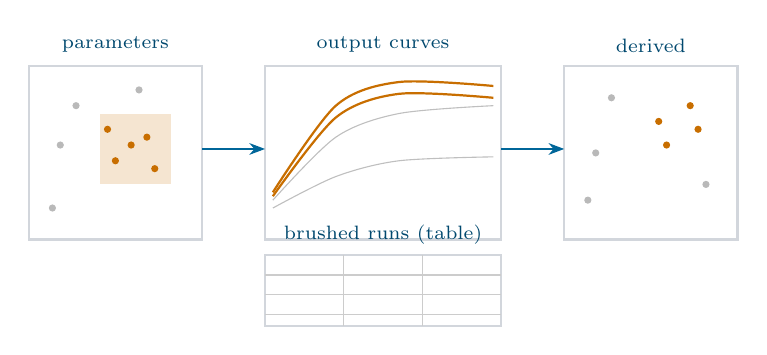
\begin{tikzpicture}[x=1cm,y=1cm,font=\scriptsize,>={Stealth[length=2mm]}]
  % ---- LEFT: parameter-space scatterplot with a brushed region ----
  \draw[rulec,thick] (0,0) rectangle (2.2,2.2);
  \node[anchor=south,tuwdark] at (1.1,2.25) {parameters};
  \fill[examorange!18] (0.9,0.7) rectangle (1.8,1.6); % brush
  \foreach \p in {(0.3,0.4),(0.6,1.7),(1.4,1.9),(0.4,1.2)}{
    \fill[gray!55] \p circle (1.3pt);}
  \foreach \p in {(1.1,1.0),(1.5,1.3),(1.0,1.4),(1.6,0.9),(1.3,1.2)}{
    \fill[examorange] \p circle (1.3pt);}
  % ---- CENTRE: curve view (output curves), brushed in orange ----
  \draw[rulec,thick] (3.0,0) rectangle (6.0,2.2);
  \node[anchor=south,tuwdark] at (4.5,2.25) {output curves};
  \draw[gray!50] plot[smooth] coordinates{(3.1,0.5)(3.9,1.3)(4.7,1.6)(5.9,1.7)};
  \draw[gray!50] plot[smooth] coordinates{(3.1,0.4)(3.9,0.8)(4.7,1.0)(5.9,1.05)};
  \draw[examorange,thick] plot[smooth]
        coordinates{(3.1,0.6)(3.9,1.7)(4.7,2.0)(5.9,1.95)};
  \draw[examorange,thick] plot[smooth]
        coordinates{(3.1,0.55)(3.9,1.55)(4.7,1.85)(5.9,1.8)};
  % ---- RIGHT: derived-output scatterplot ----
  \draw[rulec,thick] (6.8,0) rectangle (9.0,2.2);
  \node[anchor=south,tuwdark] at (7.9,2.25) {derived};
  \foreach \p in {(7.1,0.5),(7.4,1.8),(8.6,0.7),(7.2,1.1)}{
    \fill[gray!55] \p circle (1.3pt);}
  \foreach \p in {(8.0,1.5),(8.4,1.7),(8.1,1.2),(8.5,1.4)}{
    \fill[examorange] \p circle (1.3pt);}
  % ---- linking arrows ----
  \draw[->,tuwblue] (2.2,1.15) -- (3.0,1.15);
  \draw[->,tuwblue] (6.0,1.15) -- (6.8,1.15);
  % ---- data table below (brushed runs) ----
  \draw[rulec,thick] (3.0,-1.1) rectangle (6.0,-0.2);
  \foreach \y in {-0.45,-0.7,-0.95}{\draw[gray!40] (3.0,\y)--(6.0,\y);}
  \draw[gray!40] (4.0,-0.2)--(4.0,-1.1); \draw[gray!40] (5.0,-0.2)--(5.0,-1.1);
  \node[anchor=south,tuwdark] at (4.5,-0.18) {brushed runs (table)};
\end{tikzpicture}
\end{center}
\sketchnote{Ensemble CMV: left column $=$ parameter-space scatterplots/histograms
($dT_v, dT_p, P_{low},\dots$) with a brushed region; centre $=$ a curve view of
all members' output curves, brushed members in orange, context in grey; right
$=$ scatterplots of derived scalar outputs; a data table below lists the brushed
runs. Brushing any view re-highlights the same members everywhere.}

% ======================================================================
\subsection{Exam Angle}

\begin{exambox}[Set-typed data: strategy / list questions]
\textbf{``What is set-typed data and how would you visualise it?''} (1) Define:
elements with membership in multiple, possibly overlapping sets (set-typed
attribute). (2) List techniques by category: Euler/Venn, overlays
(point/region/line), matrix-based, node-link, aggregation. (3) State the
key trade-off: Euler/Venn fails beyond $\sim$3 sets (undrawable
intersections, area bias). (4) \textbf{Recommend UpSet} for many sets:
intersection matrix + sorted intersection-size bars + set-size bars; scales,
shows intersections explicitly. Mention the pie-chart pitfall and that pattern
visibility in matrices depends on ordering.
\end{exambox}

\begin{exambox}[Reading an UpSet plot -- visualisation literacy]
You may be shown an UpSet plot and asked to read it. Steps: (a) the left bars
give each \emph{set's} total size; (b) pick a column in the matrix -- the
\emph{filled} dots name the sets the elements belong to, \emph{empty} dots the
sets they do not; (c) the bar above that column gives the \emph{intersection's
size}. So ``only $B$'' $=$ one filled dot on $B$; ``$A\cap B$ but not $C$'' $=$
filled $A,B$, empty $C$; ``$A\cap B\cap C$'' $=$ all filled. The tallest
intersection bar is the dominant combination. Equivalent question for curves:
``a line brush selects which curves?'' -- all curves that \emph{cross the
line}.
\end{exambox}

\begin{exambox}[Curves \& ensembles]
Expect short-answer questions: define a \term{family of function graphs}
(many curves of one dependent variable; problem $=$ over-plotting; remedies $=$
density/banded rendering, line/composite brushing, brushing on derived curve
features in linked views). Define a \term{simulation ensemble} (many runs with
varied parameters; members multi-dimensional/time-dependent; goals $=$
parameter sensitivity, model reconstruction, representative/outlier members;
technique $=$ CMV linking parameter space $\leftrightarrow$ spatial/curve views,
aggregation, brushing across members, plus interactive ensemble steering).
\end{exambox}

\section{Visualization for Machine Learning (VIS4ML) \& Explainable AI}

\term{VIS4ML} = \emph{visualization to support machine-learning problems}. It is
the dual of \term{ML4VIS} (machine learning used to build or steer
visualizations, e.g.\ clustering and KDE used to summarize a scatterplot).
\textbf{Mnemonic:} \emph{VIS4ML} -- the visualization is the tool, the ML model
is the \emph{what} (the data); \emph{ML4VIS} -- ML is the tool inside the
visualization pipeline.

\begin{keybox}[VIS4ML in one sentence]
Use interactive visualization across the whole ML pipeline -- to understand the
\term{data}, to \term{build/debug} models, to \term{evaluate} them, and to
\term{interpret} them and build \term{trust} -- because models (and their
training data) are high-dimensional black boxes.
\end{keybox}

\subsection{Why VIS4ML: visualization in the ML pipeline}

After Sacha et al.\ (VIS4ML Ontology, 2019) the \term{what} is always
\emph{models}; visualization supports the phases of the (visual) data-science
process:

\begin{itemize}
  \item \term{Train} -- training-data inspection; training-progress inspection
    (watch the learning over epochs); interactive labeling.
  \item \term{Evaluate} -- model-quality analysis; \term{explainability};
    \term{interpretability}.
  \item \term{Use} -- what-if analysis.
\end{itemize}

Model evaluation answers three questions (a common exam framing):
\begin{enumerate}[label=(\arabic*)]
  \item \term{IF} the model learned correctly (e.g.\ confusion matrix).
  \item \term{WHAT} the model learned (e.g.\ projecting learned features).
  \item \term{WHY} the model did \emph{not} learn correctly (e.g.\
    similarity-preserving scatterplots of neuron activations).
\end{enumerate}

\begin{keybox}[VIS4ML vs.\ ML4VIS]
\term{VIS4ML}: visualization helps the ML practitioner (debug/understand the
model). \quad \term{ML4VIS}: ML helps the visualization (e.g.\
projection, clustering, KDE-thresholding to find clusters in screen space).
\end{keybox}

\subsection{Confusion matrix -- ``IF the model learned correctly''}

A \term{confusion matrix} cross-tabulates ground truth against predictions for a
classifier. Convention used in the course:
\textbf{rows = true (actual) label, columns = predicted (estimated) label};
each cell holds the frequency (count) of items.

\begin{itemize}
  \item \term{Diagonal} cells = correct predictions (true class = predicted class).
  \item \term{Off-diagonal} cells = errors; cell $(i,j)$ tells you how often
    true class $i$ was predicted as $j$, i.e.\ \emph{which classes get confused}.
  \item \term{Normalization}: dividing each row by its row sum turns counts into
    per-class recall ratios, so classes with different support are comparable
    (a stacked-bar / ``confusion star/gear'' variant shows the accumulated ratio).
\end{itemize}

\begin{center}
\begin{tabular}{c|ccc}
\toprule
 \textbf{true}$\backslash$\textbf{pred.} & $c_1$ & $c_2$ & $c_3$ \\
\midrule
$c_1$ & \textbf{200} & 5 & 4 \\
$c_2$ & 2 & \textbf{156} & 3 \\
$c_3$ & 2 & 3 & \textbf{211} \\
\bottomrule
\end{tabular}
\end{center}

\begin{center}
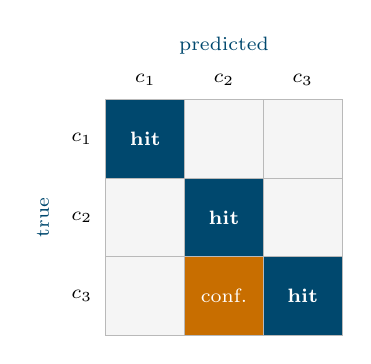
\begin{tikzpicture}[x=1cm,y=1cm,font=\scriptsize]
  % 3x3 confusion grid. row 0 = top (true c1), col 0 = left (pred c1).
  % cell(row r, col c): x = c, y = -r  (so r grows downward)
  % gray level = confusion intensity (0..1); diagonal = dark hits.
  \foreach \r in {0,1,2}{
    \foreach \c in {0,1,2}{
      \fill[gray!8] (\c,-\r) rectangle (\c+1,-\r-1);}}
  % diagonal hits (dark / bold)
  \foreach \i in {0,1,2}{
    \fill[tuwdark] (\i,-\i) rectangle (\i+1,-\i-1);}
  % bright off-diagonal confusion: true c3 (row 2) predicted c2 (col 1)
  \fill[examorange] (1,-2) rectangle (2,-3);
  % grid lines
  \foreach \k in {0,1,2,3}{
    \draw[gray!55] (\k,0)--(\k,-3);
    \draw[gray!55] (0,-\k)--(3,-\k);}
  % diagonal cell labels (hits)
  \foreach \i in {0,1,2}{
    \node[white] at (\i+0.5,-\i-0.5) {\textbf{hit}};}
  % confusion label
  \node[white] at (1.5,-2.5) {conf.};
  % column headers (predicted)
  \node[anchor=south] at (0.5,0.05) {$c_1$};
  \node[anchor=south] at (1.5,0.05) {$c_2$};
  \node[anchor=south] at (2.5,0.05) {$c_3$};
  \node[anchor=south,tuwdark] at (1.5,0.45) {predicted};
  % row headers (true)
  \node[anchor=east] at (-0.05,-0.5) {$c_1$};
  \node[anchor=east] at (-0.05,-1.5) {$c_2$};
  \node[anchor=east] at (-0.05,-2.5) {$c_3$};
  \node[rotate=90,anchor=south,tuwdark] at (-0.6,-1.5) {true};
\end{tikzpicture}
\end{center}
\sketchnote{A square grid; bold diagonal = hits; bright off-diagonal cell =
a systematic confusion (e.g.\ on MNIST many true 9's land in the ``4'' column).}

\begin{exambox}[Visualization-literacy: reading a confusion matrix]
This is a recurring exam item -- you are given a matrix and asked to read it.
\begin{itemize}
  \item \emph{``Boxing is never confused with handwaving.''} $\Rightarrow$ the
    cell (true = boxing, pred = handwaving) \textbf{is 0}. ``Never confused''
    $=$ zero off-diagonal cell. (Both directions $\to$ check both cells.)
  \item \emph{``Which class is hardest to classify?''} $\Rightarrow$ the class
    whose \textbf{diagonal value is lowest} relative to its row total, i.e.\ the
    row whose mass is \textbf{most spread} across off-diagonal columns (lowest
    recall). With normalization, the smallest diagonal percentage.
  \item \emph{``Which class is best classified?''} $\Rightarrow$ highest
    normalized diagonal entry.
\end{itemize}
\end{exambox}

\subsection{Feature vectors from neuron activations (Rauber et al.)}

Rauber et al.\ (TVCG 2017, mandatory reading) treat the \term{activations of a
layer} as a high-dimensional feature vector and project them to 2D.

\begin{itemize}
  \item For a multilayer perceptron, neuron $j$ in layer $l$ has weighted input
    $z_j^{(l)} = b_j^{(l)} + \sum_k w_{j,k}^{(l)} a_k^{(l-1)}$ and activation
    $a_j^{(l)}$ (sigmoid, ReLU $=\max(0,z)$, or softmax). The layer activation
    $\mathbf{a}^{(l)} = (a_1^{(l)},\dots,a_{N^{(l)}}^{(l)})$ is a
    \term{learned representation} of the input.
  \item These vectors are projected with a \term{similarity-preserving}
    technique (\term{t-SNE}, UMAP, or hierarchical SNE) into a scatterplot.
    Color = ground-truth class. The \emph{axes are not interpretable, but the
    instances are}.
\end{itemize}

\begin{keybox}[What the projection of activations shows]
\begin{itemize}
  \item \term{Single-color clusters} (one class = one well-separated blob)
    $\Rightarrow$ identical ground-truth classes produce similar activations
    $\Rightarrow$ \emph{solid model performance}.
  \item Class \term{separation increases with depth and with training}: deeper
    layers / later epochs separate classes more cleanly than the raw input.
  \item \term{Overlapping / mixed-color} regions $\Rightarrow$ classes the
    network cannot tell apart -- exactly the confusions seen off-diagonal in the
    confusion matrix.
  \item \term{Visual outliers} (a point of one color inside another cluster)
    flag problematic / misclassified cases (e.g.\ a ``3'' that activates like a ``5'').
\end{itemize}
Caveat (FMNIST): a similarity-preserving scatterplot \emph{alone} may not
suffice to explain patterns/outliers -- inspect representative instances too.
\end{keybox}

\subsection{Interpretability taxonomy (XAI)}

\begin{keybox}[Three orthogonal axes]
\begin{description}[leftmargin=1.3cm,style=nextline]
  \item[Scope] \term{Local} = explain the decision for a \emph{single instance};
    \term{Global} = explain the \emph{whole model} behavior. (A globally complex
    model can still have locally explainable decision boundaries.)
  \item[When] \term{Intrinsic} = the model is inherently interpretable (read the
    model itself); \term{Post-hoc} = explain after training with a separate method.
  \item[Coupling] \term{Model-specific} = exploits a known, inherently
    interpretable structure; \term{Model-agnostic} = treats the model as a
    \emph{black box} (inner structure too complex or unknown), probing only via
    inputs and outputs.
\end{description}
\end{keybox}

\term{Model-specific / intrinsic} examples: \term{linear regression}
($y=\beta_0+\beta_1 x_1+\dots+\beta_p x_p+\epsilon$; read the weights $\beta$
with confidence intervals -- but note weights mix with feature scales, so use
\emph{effect} $=\beta_j x_i^j$ plots, not raw weights, to judge contribution),
\term{decision trees} (splitting condition, Gini impurity, samples-per-class per
node), and CNN feature visualizations of spatial activations.

\begin{exambox}[Exam ``List'': name the model-agnostic methods]
\begin{enumerate}[label=\arabic*.]
  \item \term{Local perturbations} (probe one instance by editing its features).
  \item \term{LIME} -- Local Interpretable Model-agnostic Explanations.
  \item \term{SHAP} / Shapley-value feature attribution.
  \item \term{Partial Dependence Plots (PDP)} and \term{ICE} curves.
  \item \term{Counterfactual explanations}.
  \item \term{Saliency / attention maps} (gradient/attribution based).
\end{enumerate}
All are post-hoc and need only input--output access (no internal weights).
\end{exambox}

\subsection{Model-agnostic methods}

\begin{algobox}[Local perturbations / LIME (Ribeiro et al.\ 2016)]
\textbf{Idea:} explain one prediction by \emph{perturbing the input around that
instance} and observing how the black-box output changes; fit a \emph{simple,
interpretable local surrogate} (e.g.\ sparse linear model) to the
perturbed samples to approximate the decision boundary nearby.\\
\textbf{Scope / coupling:} \term{local}, \term{model-agnostic}, post-hoc.\\
\textbf{Properties:} works on \term{interpretable features} (need not be
quantitative -- e.g.\ image \term{superpixels} masked in/out, or a 3D object's
texture/hue altered). Reveals what a single decision relies on (e.g.\ a model
keying on \emph{texture rather than shape}).\\
\textbf{Hyperparameters:} perturbation/sampling neighborhood (kernel width),
number of samples, surrogate complexity (\#\,features kept).\\
\textbf{Pitfalls:} explanation depends on the (arbitrary) neighborhood
definition; only locally faithful; unstable -- nearby instances can get
different explanations.
\end{algobox}

\begin{algobox}[SHAP / Shapley feature attribution]
\textbf{Idea:} from cooperative game theory -- distribute the prediction fairly
among features as \term{Shapley values}, the average marginal contribution of a
feature over all orderings of feature coalitions.\\
\textbf{Scope / coupling:} \term{local} attribution (aggregates to global),
\term{model-agnostic}.\\
\textbf{Properties:} additive, consistent attribution per feature; positive vs.\
negative contributions to a specific prediction.\\
\textbf{Pitfalls:} exact computation is exponential in \#\,features (approximated
in practice); like PDP it can be misled by correlated features.
\end{algobox}

\begin{algobox}[Partial Dependence Plot (PDP) -- Krause et al.\ 2016]
\textbf{Idea:} the \emph{marginal effect} of one (or two) feature(s) on the
prediction, \emph{averaged over all other features' values in the data}.
Systematically set the chosen feature to each level (try all recorded levels for
categorical features), re-predict for every training row, average the responses,
and plot level vs.\ average response.\\
\textbf{Scope / coupling:} \term{global}, \term{model-agnostic}.\\
\textbf{Reading:} a curve (quantitative feature) or bar chart (categorical),
e.g.\ predicted bike rentals rise with temperature, fall with humidity/wind.\\
\textbf{Hyperparameters:} which feature(s); grid resolution.\\
\textbf{Pitfall:} \term{assumes feature independence} -- averaging over the
marginal can create unrealistic feature combinations and hide heterogeneous
effects. \term{ICE (Individual Conditional Expectation)} curves are the
\emph{per-instance} variant: one line per data point instead of the average,
exposing interactions the averaged PDP masks.
\end{algobox}

\begin{algobox}[Counterfactual explanations]
\textbf{Idea:} the \term{minimal set of changes to the feature values} that
\emph{flips} the prediction to a \emph{different output} -- the smallest
perturbation that crosses the decision boundary.\\
\textbf{Scope / coupling:} \term{local}, \term{model-agnostic}.\\
\textbf{Properties:} \emph{not unique} -- many valid counterfactuals exist
(several different small changes can each flip the label), so often a set is
sought. A good counterfactual should be \term{plausible / realistic} (lie on the
data manifold) and \term{sparse / close} (change few features, stay near the
original). What-if tools (ViCE, Gomez et al.\ 2020) show the change as a glyph
against the feature's density distribution.\\
\textbf{Pitfalls:} can be unrealistic if plausibility is not enforced;
multiplicity makes ``the'' explanation ambiguous.
\end{algobox}

\begin{exambox}[Counterfactual true/false MCQ]
\begin{itemize}
  \item ``A counterfactual is the \emph{minimal} set of changes that flips the
    prediction.'' $\Rightarrow$ \textbf{TRUE}.
  \item ``A counterfactual is the \emph{maximum} change to feature values.''
    $\Rightarrow$ \textbf{FALSE} (it is minimal, not maximal).
  \item ``There is exactly \emph{one} counterfactual per instance.''
    $\Rightarrow$ \textbf{FALSE} (counterfactuals are not unique).
  \item ``Counterfactuals should be \emph{plausible}.'' $\Rightarrow$
    \textbf{TRUE}.
\end{itemize}
\end{exambox}

\term{Saliency / attention maps} (brief): post-hoc, typically \term{local} maps
that highlight which input regions (pixels, tokens) most influenced a single
prediction -- a heatmap overlay answering ``where did the model look?''.

\subsection{Surrogate models}

A \term{surrogate model} is a simple, interpretable model (linear model, shallow
tree) trained to mimic a black-box model's input--output behavior. Used
\emph{locally} (LIME's local surrogate around one instance) or \emph{globally},
surrogates make black-box models interpretable by substituting a transparent
approximation that humans can read.

\begin{pitfall}[Common confusions]
\begin{itemize}
  \item Confusion-matrix axes: \emph{rows = truth, columns = prediction}.
    Reversing them flips your reading of every off-diagonal cell.
  \item PDP/SHAP \emph{assume feature independence}; do not claim PDP gives
    per-instance behavior -- that is ICE.
  \item Counterfactual = \emph{minimal} change and \emph{not unique}; ``maximum''
    or ``only one'' are wrong.
  \item Model-\emph{agnostic} $\ne$ model-\emph{specific}: agnostic = black-box,
    input/output only; specific = exploits a known interpretable structure.
\end{itemize}
\end{pitfall}

\section{Evaluation and Validation}

How do you know your visualization actually \term{amplifies cognition}? You
cannot rely on intuition: the design space is huge and most designs are
ineffective. Evaluation answers ``how well does my visualization work?''; the
exam phrases this as ``how will you validate your proposed solution?''. The
central framework is Munzner's \term{nested model} (Munzner, TVCG 2009; book
Chapter~4), which tells you, level by level, what can go wrong (\term{threats})
and which method addresses each threat.

\subsection{Munzner's Nested Model: Four Levels}

Vis design is split into four \term{cascading, nested} levels. The output of an
\term{upstream} (outer) level is the input to the \term{downstream} (inner) one.
A block is the outcome of design at a level. The big consequence of nesting: a
\term{poor choice at an upstream level cascades to all downstream levels}, so a
perfect idiom and algorithm cannot save a wrong abstraction.

\begin{keybox}[The four levels (outer $\rightarrow$ inner)]
\begin{enumerate}[label=\arabic*.]
  \item \term{Domain situation} (\emph{why} / who): target users, their domain,
        questions, data. Blocks are \emph{identified}.
  \item \term{Data / task abstraction} (\emph{what} \& \emph{why}): map
        domain-specific data + questions into domain-independent data types and
        abstract tasks. Tasks are identified; data is \emph{designed}.
  \item \term{Visual encoding / interaction idiom} (\emph{how}): how to draw it
        (visual encoding) and how the user changes it (interaction). Blocks are
        \emph{designed}.
  \item \term{Algorithm}: efficient automatic procedure that instantiates the
        idiom. Blocks are \emph{designed}.
\end{enumerate}
\end{keybox}

\begin{center}
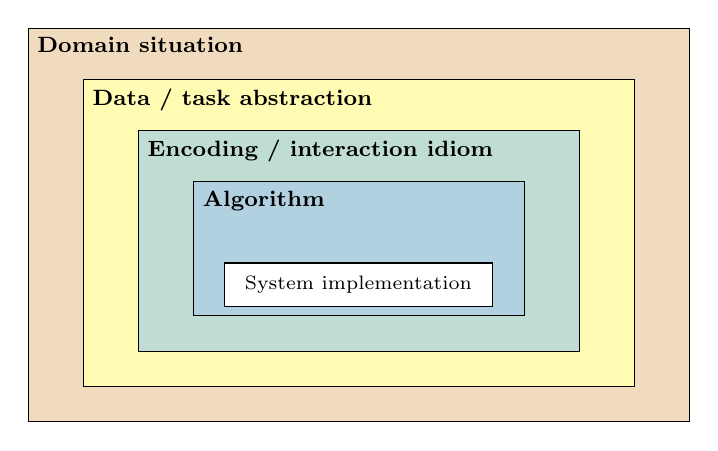
\begin{tikzpicture}[font=\footnotesize]
  \node[draw, fill=examorange!25, minimum width=8.4cm, minimum height=5.0cm, anchor=south west] (l1) at (0,0) {};
  \node[anchor=north west] at (l1.north west) {\bfseries Domain situation};
  \node[draw, fill=yellow!30, minimum width=7.0cm, minimum height=3.9cm, anchor=south west] (l2) at (0.7,0.45) {};
  \node[anchor=north west] at (l2.north west) {\bfseries Data / task abstraction};
  \node[draw, fill=keygreen!25, minimum width=5.6cm, minimum height=2.8cm, anchor=south west] (l3) at (1.4,0.9) {};
  \node[anchor=north west] at (l3.north west) {\bfseries Encoding / interaction idiom};
  \node[draw, fill=tuwblue!30, minimum width=4.2cm, minimum height=1.7cm, anchor=south west] (l4) at (2.1,1.35) {};
  \node[anchor=north west] at (l4.north west) {\bfseries Algorithm};
  \node[draw, fill=white, minimum width=3.4cm, minimum height=0.55cm] at (4.2,1.75) {\scriptsize System implementation};
\end{tikzpicture}
\end{center}
\sketchnote{four nested rectangles, outer to inner: Domain $\supset$
Data/Task abstraction $\supset$ Encoding/Interaction idiom $\supset$ Algorithm,
with ``System implementation'' as the innermost white box.}

\subsubsection{Threats and Validation per Level}

Each level has its own \term{threat} (the way that level can fail) and its own
\term{validation method}. Crucially, validations are either \term{immediate}
(can be done at that level, before downstream levels exist) or \term{downstream}
(require the inner levels to be implemented first, so they cannot be done until
the system runs). Immediate validation only gives \emph{partial} evidence;
downstream validation is necessary for a full demonstration.

\begin{center}\footnotesize
\begin{longtable}{@{}p{2.6cm}p{3.1cm}p{4.2cm}p{2.2cm}@{}}
\toprule
\textbf{Level} & \textbf{Threat} & \textbf{Validation method} & \textbf{Timing}\\
\midrule
\endhead
Domain situation & Wrong problem (you misunderstood their needs) &
  Observe / interview target users (contextual inquiry, field study) & Immediate\\
 & & Measure / observe \term{adoption rates} of deployed tool & Downstream\\
\addlinespace
Data / task abstraction & Wrong abstraction (you show them the wrong thing) &
  Test on \term{real target users doing their own tasks}; collect anecdotal
  evidence of utility & Downstream\\
 & & Field study of the deployed system in real workflow & Downstream\\
\addlinespace
Encoding / interaction idiom & Wrong idiom (the way you show it does not work) &
  \term{Justify} design vs.\ alternatives using perceptual / cognitive
  principles; heuristic / expert review & Immediate\\
 & & Qualitative / quantitative result-image analysis & Downstream\\
 & & \term{Lab study}: controlled experiment measuring human \term{time and
  errors} for a task & Downstream\\
\addlinespace
Algorithm & Wrong / slow algorithm (your code is too slow or incorrect) &
  Analyze \term{computational complexity} & Immediate\\
 & & Measure wall-clock \term{system time and memory}; compare to benchmarks & Downstream\\
\bottomrule
\end{longtable}
\end{center}

\begin{pitfall}[Mismatch between claim and method]
A weak project validates at the wrong level. You \emph{cannot} validate a new
\emph{encoding idiom} with wall-clock algorithm timings, and you \emph{cannot}
address a mischaracterized \emph{task} with a lab study whose task is dictated
by the experimenter. \term{Choose the validation method according to your
contribution claim.} Informal usability studies are done \emph{upstream} of a
real study (to fix usability bugs first) but are \emph{not} themselves a
validation method.
\end{pitfall}

\subsection{Types of Evaluation}

Two broad styles, often combined (mixed-methods):
\begin{itemize}
  \item \term{Quantitative}: numeric measures, statistical testing (lab/online
        experiments, eye tracking metrics, algorithm benchmarks).
  \item \term{Qualitative}: observations, interviews, open-ended feedback,
        coded transcripts.
\end{itemize}

\begin{keybox}[Method catalogue (by number of people involved, large $\rightarrow$ few)]
\begin{itemize}
  \item \term{Controlled experiment / lab study}: comparative, in a controlled
        setting; measures performance. Strongest for comparing encoding /
        interaction choices.
  \item \term{Crowdsourcing study} (Mechanical Turk, Prolific): web workers,
        micro-payments. + diverse/large population (ecological validity, large
        design-space coverage); $-$ no control over conditions. Needs
        \term{attention checks} / instructional manipulation checks.
  \item \term{Eye tracking study}: records fixations, saccades, scanpaths;
        metrics per \term{area of interest (AOI)}.
  \item \term{Insight-based study}: no predefined tasks; users explore until
        ``done'', think-aloud, insights \term{coded} and quantified, treated as
        dependent variables (North, 2006).
  \item \term{Expert / heuristic evaluation}: ``discount'' method, $\sim$5
        experts find $>$75\% of problems (Nielsen); checks against vis
        heuristics (Shneiderman's mantra, perception, color blindness). ICE-T
        questionnaire operationalizes value $=$ Time $+$ Insight $+$ Essence $+$
        Confidence. Cognitive walkthrough $=$ expert steps through specific tasks.
  \item \term{Usability study}: uncovers usability problems; user need not be in
        the target domain. Done before a validating study, not instead of it.
  \item \term{Field study}: qualitative, on-site, users work on their own
        problems in their normal environment. ``Gold standard but time
        consuming''. Validates domain (existing practice) or abstraction
        (changed behavior after deployment).
  \item \term{Case study / qualitative result inspection}: no experiment; reader
        inspects result images / a walkthrough (comparative or isolated). A
        reasonable middle ground.
  \item \term{Qualitative coding}: iterative characterization of transcripts /
        video / field notes. \term{Open coding}: label each phenomenon
        (concept), group into categories, build a \term{code book}. Quality
        assurance via multiple coders and \term{inter-rater reliability}.
  \item \term{Longitudinal study}: observes use over an extended period (e.g.\
        adoption, field deployment over time).
  \item \term{Algorithmic / benchmark evaluation}: complexity analysis plus
        wall-clock time and memory on standard benchmarks.
\end{itemize}
\end{keybox}

\subsection{Controlled Experiment Design}

A controlled experiment isolates the effect of one (or few) factors on measured
performance, ensuring \term{internal validity}.

\begin{keybox}[Anatomy of a controlled experiment]
\begin{itemize}
  \item \term{Hypothesis}: logical, precise, testable, justifiable (state the
        expected direction).
  \item \term{Independent variables (factors)}: what you deliberately vary
        (e.g.\ visualization method, task, data size, population). \term{Levels}
        $=$ number of variations per factor $=$ test conditions.
  \item \term{Dependent variables}: the measured outcome (user performance).
  \item \term{Control variables}: held constant (e.g.\ display size, data
        characteristics).
  \item \term{Random variables}: randomly varied across conditions (e.g.\ data
        variations).
  \item \term{Confounding variables}: unmeasured variable that unintentionally
        correlates with an IV; must be avoided to keep internal validity
        (example: crosses are harder to click than circles, so a difference
        attributed to ``encoding'' is really about clickability).
\end{itemize}
\end{keybox}

\begin{exambox}[List: typical dependent variables]
\begin{itemize}
  \item \term{Task completion time} (speed; ideally only the actual solving
        time, shown after instructions).
  \item \term{Accuracy / error rate} -- including \term{false positives} and
        \term{false negatives}.
  \item Number of interaction steps / actions (logged clicks, mouse moves).
  \item \term{Subjective preference / satisfaction} (Likert scale,
        questionnaires e.g.\ System Usability Scale).
  \item \term{Confidence}, \term{memorability/recall}, and \term{insight count}
        (for exploratory tasks).
  \item Eye-tracking measures: first-fixation time, number of fixations in an
        AOI, saccade amplitude, scanpath transitions.
\end{itemize}
\end{exambox}

\subsubsection{Experimental Design and Statistics}
\begin{itemize}
  \item \term{Within-subjects} (repeated measures): every participant does every
        condition. Watch for \term{learning effect} $\rightarrow$
        \term{counterbalance} condition order (e.g.\ \term{Latin square}).
  \item \term{Between-subjects}: each group does only one variation of a factor
        (no learning effect, but needs more participants, more variance).
  \item \term{Mixed design}: combination of the two.
  \item \term{Power analysis} decides the number of participants given
        $\alpha$ (Type I error), $\beta$ (Type II error / power $=1-\beta$) and
        effect size. Increase power by more participants, fewer conditions,
        larger effect size, lower variance (homogeneous population, removing
        outliers, more control variables).
  \item \term{Statistical significance}: check distribution (e.g.\ Shapiro test);
        if normal use a (matched) $t$-test / ANOVA with post-hoc (Tukey),
        otherwise a non-parametric test (Wilcoxon signed-rank).
\end{itemize}

\begin{pitfall}[Useless user studies]
Foregone conclusions, fishing for results, confounding factors, experimenter
bias, lack of external validity (not generalizable), lack of practical
significance, lack of power. Antidote: define research questions / success
criteria \emph{before} you start; then the validation method is usually obvious.
\end{pitfall}

\subsection{Worked Example: Encoding Classes in Static Scatterplots}

\emph{Template answer to ``design a user study to compare visual encodings of
classes (sets) in a static scatterplot''.} The task is to mark group membership
of points; candidate channels are \term{color}, \term{shape}, \term{connection}
(Gestalt), and \term{redundant combinations}.

\begin{keybox}[Full study template]
\textbf{Hypotheses} (directional, justified by channel rankings / perception):
\begin{itemize}
  \item H1: \term{color} $>$ \term{shape} -- color (a position-free identity
        channel) is more effective than shape per the channel ranking.
  \item H2: \term{connection} $>$ color -- connection lines (Gestalt grouping)
        beat color for grouping tasks.
  \item H3: \term{redundant} $>$ single -- redundant encoding (e.g.\
        color $+$ shape) beats either single channel (less channel interference).
\end{itemize}
\textbf{Independent variable}: encoding $\in$ \{color, shape, connection,
combinations\} (one factor, $\geq$4 levels).\\
\textbf{Dependent variables}: \term{accuracy} -- with \term{false positives}
(items wrongly marked) and \term{false negatives} (items missed) -- and
\term{task completion time}; optionally subjective preference.\\
\textbf{Task}: ``click / select all items of a given class.''\\
\textbf{Confounds to avoid}: marks differ in clickability (crosses are harder to
click than circles) $\rightarrow$ equalize target size / hit area; also label
readability, visual appeal.\\
\textbf{Control variables}: number of classes, class balance, number of points,
point distribution, chart size, display.\\
\textbf{Design}: within-subjects with counterbalanced order; power analysis for
$N$; significance test on accuracy and time.
\end{keybox}

\subsection{Effectiveness: Why We Visualize Defines the DV}

The choice of task and dependent variable is not arbitrary: it follows from
\term{why} people use the visualization. Munzner's task abstraction distinguishes
low-level \term{actions} -- \term{identify}, \term{compare}, \term{summarize} --
from the data \term{targets} the user is after -- \term{trends}, \term{outliers},
\term{features}, distributions, correlation, similarity, topology / paths.
Effectiveness means: faster to interpret, supports more distinctions, fewer
errors. So a ``find the outlier'' goal becomes an \emph{identify} task with
accuracy $+$ time as DVs; a ``which is bigger'' goal becomes a \emph{compare}
task. Match the measured DV to the real low-level action, or the study answers
the wrong question.

\begin{exambox}[``How would you validate your project / design a user study?'']
A safe full-marks structure:
\begin{enumerate}[label=\arabic*.]
  \item \textbf{Locate the contribution in the nested model} and pick the
        matching method (encoding/interaction claim $\rightarrow$ lab study;
        algorithm claim $\rightarrow$ benchmarks; problem claim $\rightarrow$
        field study; adoption $\rightarrow$ longitudinal).
  \item \textbf{State a precise, justified hypothesis} and the high-level goal
        (exploration / confirmation / presentation).
  \item \textbf{Name IVs and their levels} (encoding/technique, data size,
        task), \textbf{DVs} (completion time, accuracy with FP/FN, preference,
        insight count), \textbf{control} and \textbf{confounding} variables.
  \item \textbf{Choose design} (within- vs between-subjects, counterbalancing),
        \textbf{participants} via power analysis, and the \textbf{statistical
        test}.
  \item Add \textbf{qualitative data} (think-aloud, semi-structured interview,
        coding) to explain outliers and put numbers in context.
  \item Discuss \textbf{threats / limitations}: representativeness of tasks,
        layout, number and background of users; whether ``time $+$ error tell
        the whole story''.
\end{enumerate}
Remember the two big takeaways: \emph{validation method follows the contribution
claim}, and \emph{upstream errors cascade downstream}.
\end{exambox}

\section{Exam Question-Type Playbook}
\label{sec:playbook}

This section gives, for each of the nine exam question types foreshadowed by
the professor, (a) what it asks, (b) a step-by-step answer strategy, (c) the
rubric / point deductions to avoid, and (d) a short worked mini-example.
The detailed theory lives in the earlier sections; here we drill the
\emph{format of the answer}.

% =====================================================================
\subsection{Type 1 -- Visualization Literacy (read a chart)}

\textbf{What it asks.} Given a concrete visualization (boxplot, bar/stacked/
grouped bar, histogram, pie, line chart, scatterplot, parallel coordinates,
star/radar, SPLOM, heatmap, confusion matrix, choropleth, node-link, adjacency
matrix, treemap, mosaic, UpSet, arc diagram, 3D scatter), report observations
in free form or judge true/false statements.

\begin{exambox}[Answer strategy]
\begin{enumerate}[leftmargin=1.4em]
  \item \term{Identify the chart} and what is mapped to each channel
        (x, y, colour, size, area, position).
  \item \term{Read the encoding back to data}: a tall bar = large value,
        dark heatmap cell = large value, wide mosaic tile = large marginal.
  \item For \term{distributions} (box/histogram): state median, spread/IQR,
        skew, outliers, multimodality.
  \item For \term{relations} (scatter/SPLOM/PCC): state correlation sign,
        clusters, outliers, trends.
  \item For \term{confusion matrices}: diagonal = correct; off-diagonal cell
        $(i,j)$ = class $i$ predicted as $j$. ``Hardest to classify'' = row
        with smallest diagonal / most off-diagonal mass.
  \item Answer each T/F by tracing the exact cell / mark, not intuition.
\end{enumerate}
\end{exambox}

\begin{pitfall}
Confusing rows vs.\ columns in a confusion matrix (true class is usually the
row). Reading area as length (pie/treemap/mosaic encode area, which is
perceptually weak). Asserting correlation from a single outlier. Forgetting
that a log axis compresses large values.
\end{pitfall}

\textit{Mini-example.} Confusion matrix: cell (boxing, handwaving)$=0$
$\Rightarrow$ ``boxing is never confused with handwaving'' is \term{True}.
The class with the smallest diagonal entry relative to its row sum is
``jogging'' $\Rightarrow$ ``jogging is hardest to classify'' is \term{True}.

% =====================================================================
\subsection{Type 2 -- Visualization Algorithms (describe / sketch / MCQ)}

\textbf{What it asks.} Describe, sketch, or answer multiple-choice on the
properties and hyperparameters of a named algorithm: recursive subdivision
(mosaic, treemap), just-noticeable-difference, scagnostics, class consistency,
PCA, MDS, t-SNE, UMAP, hexbin, KDE, data cubes, parallel aggregation, feature
vectors, local perturbations, partial dependence, counterfactuals,
force-directed / layered / morphing / foresighted graph layout.

\begin{exambox}[Answer strategy]
\begin{enumerate}[leftmargin=1.4em]
  \item State the \term{core idea} in one sentence (input $\to$ output).
  \item Name the \term{key hyperparameters} and the effect of each.
  \item State \term{properties}: linear vs.\ nonlinear, deterministic vs.\
        stochastic, preserves global vs.\ local structure, complexity.
  \item If asked to sketch, draw axes, a few labelled points, and the
        result (e.g.\ the projection line for PCA, the binned grid for hexbin).
\end{enumerate}
\end{exambox}

\begin{pitfall}
Claiming t-SNE/UMAP distances or cluster \emph{sizes} are meaningful (they are
not). Saying PCA is nonlinear. Forgetting t-SNE/UMAP are stochastic
(need a seed) and perplexity / $n\_neighbors$ controls local-vs-global balance.
See the Algorithm Cheat-Sheet (Section~\ref{sec:algocheat}) for the full table.
\end{pitfall}

\textit{Mini-example.} ``Sketch the 1D PCA projection of a 2D point cloud.''
$\Rightarrow$ draw the cloud, the first principal axis along the direction of
maximum variance, and the points projected (dropped perpendicularly) onto it.

% =====================================================================
\subsection{Type 3 -- Visualization Strategy (data + task $\to$ design)}

\textbf{What it asks.} Given a dataset and an analysis task, propose and justify
data processing + visual design + interaction design, and defend it against
alternatives. Data may be multivariate, unstructured, multidimensional, tall,
a large graph, set-typed, a dynamic graph, or an ML model.

\begin{exambox}[Reusable 5-step strategy template]
\begin{enumerate}[leftmargin=1.4em]
  \item \term{Identify data type \& task.} Name cardinality (tall? wide?),
        attribute types, and the analytic goal (overview, compare, find
        outliers, track over time).
  \item \term{Preprocessing.} Name the \emph{scalability challenge} explicitly
        (perceptual: overplotting; interactive: latency). Pick the matching
        tool: spatial/temporal \term{binning} + \term{aggregation} for
        perceptual scalability; a \term{data cube} / pre-aggregation for
        interactive scalability; \term{sampling} or \term{dimensionality
        reduction} where appropriate.
  \item \term{Visual encoding.} Name the \emph{marks} and \emph{channels} and
        the \emph{colour map} (sequential for ordered magnitude, diverging for
        signed, categorical for nominal).
  \item \term{Interaction.} Name techniques: \term{linked (coordinated) views},
        \term{brushing}, \term{filtering}, \term{details-on-demand},
        zoom/pan, level-of-detail.
  \item \term{Justify vs.\ alternatives.} Say why the chosen encoding beats a
        plausible competitor (e.g.\ binned map vs.\ raw points; choropleth vs.\
        hexbin; line chart vs.\ heatmap).
\end{enumerate}
\end{exambox}

\begin{pitfall}
Deductions: not identifying the scalability challenge; proposing no linked
views; ineffective processing (e.g.\ raw KDE on 10M points); doing only spatial
\emph{or} temporal binning when both are needed; not naming the visual encoding
(marks/channels); not mentioning binning/aggregation; not naming the
interaction design; non-optimal colour mapping (e.g.\ rainbow for magnitude).
\end{pitfall}

\textit{Mini-example.} 10M-row table of EU traffic accidents (ID, lon, lat,
year): spatial + temporal binning (perceptual scalability) backed by a data
cube (interactive scalability); two linked views, a hexbin/choropleth map
(sequential colour, regions brushable) and a temporal line chart/histogram
(year ranges brushable). Worked in full in Section~\ref{sec:practice}.

% =====================================================================
\subsection{Type 4 -- Design \& Validation Strategy (user study)}

\textbf{What it asks.} Given a research topic, design a validation / user study:
state hypotheses and identify independent, dependent, controlled, and
confounding variables.

\begin{exambox}[Answer strategy]
\begin{enumerate}[leftmargin=1.4em]
  \item \term{Hypothesis} (directional, falsifiable): ``Encoding A yields
        faster/more accurate task performance than encoding B.''
  \item \term{Independent variable (IV)}: what you manipulate (the encoding /
        technique), with its levels.
  \item \term{Dependent variables (DV)}: what you measure -- task completion
        \emph{time}, \emph{accuracy / error rate}, subjective preference,
        cognitive load, confidence.
  \item \term{Controlled variables}: held constant (dataset size, screen,
        task type, training).
  \item \term{Confounds}: learning/order effects (counterbalance, e.g.\ Latin
        square), fatigue, individual differences (within-subjects design).
  \item State \term{design}: within- vs.\ between-subjects, \#participants,
        analysis (ANOVA / t-test).
\end{enumerate}
\end{exambox}

\begin{pitfall}
Mixing up IV and DV. Forgetting to control dataset/task so the encoding is the
only thing varying. No mention of order/learning effects or counterbalancing.
Vague, non-measurable DVs.
\end{pitfall}

\textit{Mini-example.} ``Are class-by-colour or class-by-shape scatterplots more
effective?'' IV = encoding (colour vs.\ shape vs.\ both); DV = class-membership
judgment time \& accuracy; control point count/overlap; counterbalance order.

% =====================================================================
\subsection{Type 5 -- Critique \& Suggestions}

\textbf{What it asks.} Discuss strengths/problems of a given visualization and
suggest better encodings, using the design vocabulary.

\begin{exambox}[Critique checklist]
\begin{enumerate}[leftmargin=1.4em]
  \item \term{Data-ink ratio} / chartjunk: is ink doing data work?
  \item \term{Expressiveness}: does it show all and only the data
        (no spurious order on nominal data)?
  \item \term{Effectiveness} (Stevens' power law, channel ranking):
        position $>$ length $>$ angle/area $>$ colour. Is the most important
        attribute on the strongest channel?
  \item \term{Hidden transformations}: implicit aggregation, normalization,
        log axes, truncated baselines.
  \item \term{Lie factor} / 3D distortion / non-zero baseline.
  \item \term{Colour}: sequential vs.\ diverging vs.\ categorical;
        perceptual uniformity; rainbow problems.
  \item \term{Channel interference} / ordering.
  \item \term{Suggest} a concrete alternative encoding.
\end{enumerate}
\end{exambox}

\begin{pitfall}
Listing principles without applying them to \emph{this} chart. Forgetting to
propose a concrete fix. Calling all 3D bad without naming the actual problem
(occlusion, perspective distortion, foreshortening).
\end{pitfall}

\textit{Mini-example.} A rainbow choropleth of unemployment: rainbow is not
perceptually ordered nor uniform $\Rightarrow$ replace with a single-hue
sequential map; mention simultaneous-contrast and colour-blind safety.

% =====================================================================
\subsection{Type 6 -- Alternatives (compare two views)}

\textbf{What it asks.} Given two visualizations of the same data, discuss
pros/cons (classic: parallel coordinates vs.\ SPLOM).

\begin{exambox}[Answer strategy]
Make a 2-column pro/con table on shared axes: \term{scalability} (\#dims,
\#points), \term{task fit} (pairwise correlation vs.\ multivariate profiles /
clusters), \term{clutter / overplotting}, \term{axis ordering effects},
\term{interaction} needs. Conclude with ``use X when task is\ldots, Y when\ldots''.
\end{exambox}

\begin{pitfall}
Only listing features of each without comparing them on the same criteria, or
not tying the recommendation to a \emph{task}.
\end{pitfall}

\textit{Mini-example.} SPLOM shows all pairwise correlations but costs
$O(d^2)$ panels; PCC scales to more dimensions in one view and shows
multivariate profiles/clusters but suffers ordering effects and line clutter.

% =====================================================================
\subsection{Type 7 -- Transfer / Sketch}

\textbf{What it asks.} Transfer one representation to another and sketch it
(e.g.\ a number array $\to$ histogram + boxplot).

\begin{exambox}[Answer strategy]
Extract the summary statistics the target needs, then draw axes and the marks.
For a boxplot: sort, find min, Q1, median, Q3, max, fence outliers at
$1.5\,\mathrm{IQR}$. For a histogram: choose bins, count, draw bars.
Always \term{label the axes and key values}.
\end{exambox}

\begin{pitfall}
Unlabelled axes; wrong quartile placement; ignoring outliers; bins that hide
the distribution shape.
\end{pitfall}

\textit{Mini-example.} Array $\{1,2,2,3,9\}$: median $=2$, Q1$=2$, Q3$=3$,
$9$ is an outlier ($> Q3+1.5\,\mathrm{IQR}$); histogram is right-skewed.

% =====================================================================
\subsection{Type 8 -- Mapping Data Items Between Views}

\textbf{What it asks.} A data item highlighted in one view; mark the same item
in a paired view. Pairs: scatterplot$\leftrightarrow$PCC;
PCC$\leftrightarrow$star plot; heatmap$\leftrightarrow$grouped/stacked bars;
node-link$\leftrightarrow$adjacency matrix; treemap$\leftrightarrow$rectilinear
node-link tree.

\begin{exambox}[Answer strategy]
Recover the item's \emph{coordinates / attribute values} from the source view,
then find the mark with those same values in the target. A scatter point
$(x,y)$ becomes the PCC polyline passing through $x$ on axis~1 and $y$ on
axis~2; a heatmap cell becomes one bar in the corresponding bar group; a
node becomes the matching row+column of the adjacency matrix; a treemap
rectangle becomes the corresponding leaf in the node-link tree.
\end{exambox}

\begin{pitfall}
Reading the wrong axis in PCC; confusing a node's row/column in the adjacency
matrix; matching by colour alone when colour is reused.
\end{pitfall}

\textit{Mini-example.} Outlier point top-right of a scatter $\to$ the PCC
polyline that is high on both corresponding axes.

% =====================================================================
\subsection{Type 9 -- List / Enumerate}

\textbf{What it asks.} Enumerate concepts: raw-data issues; scalability factors;
latency sources; graph-drawing aesthetics; no-preprocessing overplotting fixes;
model-agnostic interpretability methods; set-typed visualization techniques;
validation methods; typical user-study dependent variables.

\begin{exambox}[Answer strategy]
Give a \emph{bulleted} list with a one-line gloss per item; aim for breadth
(many items) over depth. The complete memorizable lists are in
Section~\ref{sec:lists}.
\end{exambox}

\begin{pitfall}
Writing prose instead of a list; giving too few items; padding with synonyms of
the same concept.
\end{pitfall}

\textit{Mini-example.} Overplotting fixes needing no preprocessing:
transparency (alpha), smaller marks, jitter, open glyphs --- vs.\ binning/DR
which \emph{do} require preprocessing.

\section{Algorithm Cheat-Sheet}
\label{sec:algocheat}

A compact one-row-per-algorithm reference for the ``describe / sketch / MCQ''
question type. Detailed treatments are in Sections~7--11; this is the revision
sheet. Sketch boxes follow for the algorithms where a drawing matters.

\renewcommand{\arraystretch}{1.25}
\begin{longtable}{@{}>{\raggedright\arraybackslash}p{2.5cm}
                     >{\raggedright\arraybackslash}p{4.3cm}
                     >{\raggedright\arraybackslash}p{3.6cm}
                     >{\raggedright\arraybackslash}p{4.6cm}@{}}
\toprule
\textbf{Algorithm} & \textbf{Core idea} & \textbf{Key hyperparameters} &
\textbf{Key properties / pitfalls}\\
\midrule
\endfirsthead
\toprule
\textbf{Algorithm} & \textbf{Core idea} & \textbf{Key hyperparameters} &
\textbf{Key properties / pitfalls}\\
\midrule
\endhead
\bottomrule
\endfoot

Recursive subdivision (mosaic) & Split a rectangle by category proportions,
alternating axes per variable & Variable order; spacing & Tile area = joint
frequency; order changes layout; reads marginals/conditionals\\

Recursive subdivision (treemap) & Recursively nest rectangles sized by a
hierarchy's leaf values & Tiling (slice-and-dice, squarified); layout order &
Area = value; squarified gives good aspect ratios; deep hierarchies hard to
read; area is a weak channel\\

Just-noticeable-difference (JND) & Smallest stimulus change a viewer can
detect & (Weber fraction $k$) & Weber's law: $\Delta I / I = k$; motivates
perceptually uniform colour/size scales\\

Scagnostics & Graph-theoretic measures summarizing a scatterplot's shape &
(Binning grid; measure set) & Outlying, skewed, clumpy, sparse, striated,
convex, skinny, stringy, monotonic; used to rank SPLOM panels\\

Class consistency & Quality metric: do class labels agree with spatial
structure of a projection? & Distance/centroid criterion & Higher = classes
form separable clusters; used to evaluate/rank DR layouts\\

PCA & Linear projection onto orthogonal directions of max variance &
\#components $k$ & Linear, deterministic; preserves global variance; axes
interpretable; misses nonlinear structure\\

MDS & Embed so low-D distances match high-D (dis)similarities & metric vs.\
non-metric; \#dims; stress & Preserves pairwise distances; classical MDS
$\approx$ PCA; can be slow; stress measures distortion\\

t-SNE & Match neighbour probability distributions (high-D vs.\ low-D),
minimize KL & \term{perplexity}; learning rate; iterations; seed &
Nonlinear, stochastic; preserves local clusters; \emph{cluster sizes \&
between-cluster distances not meaningful}\\

UMAP & Build a fuzzy $k$-NN graph, optimize a low-D layout of it &
\term{$n\_neighbors$}; \term{min\_dist}; \#dims; seed & Nonlinear,
stochastic; faster than t-SNE; better global structure; sizes/distances still
unreliable\\

Hexagon binning & Aggregate points into hexagonal bins, encode count by
colour & bin size / \#bins & Fixes overplotting (perceptual scalability);
hexagons tile uniformly, less axis bias than squares\\

Kernel density estimation & Sum smooth kernels over points to estimate a
density & \term{bandwidth}; kernel shape & Bandwidth too small = spiky, too
large = oversmoothed; $O(n)$ per eval -- costly on tall data\\

Multi-dim tables / data cubes & Pre-aggregate measures over dimension
combinations for fast queries & dimensions; hierarchies; measures &
Interactive scalability: slice/dice/roll-up/drill-down in $O(1)$; storage
grows with dimensions\\

Parallel aggregation & Distribute aggregation over partitions, combine
partial results & \#partitions & Scales aggregation to tall data; basis of
data-cube construction; needs associative aggregates\\

Feature vectors (neuron activations) & Represent an input by a layer's
activation vector & layer choice; (DR for display) & Used to inspect what a
network ``sees''; high-D, usually projected with t-SNE/UMAP\\

Local perturbations (LIME) & Perturb one input, fit a simple local surrogate &
\#samples; kernel width; surrogate & Model-agnostic, \emph{local} explanation;
unstable to sampling; not globally faithful\\

Partial dependence (PDP) & Average model output while sweeping one feature
over its range & feature(s); grid resolution & Global, model-agnostic; assumes
feature independence; can hide interactions (ICE curves fix this)\\

Counterfactual explanation & Smallest input change that flips the prediction &
distance metric; target class; sparsity & ``Change X to get outcome Y'';
should be close, sparse, actionable, plausible; many valid counterfactuals\\

Force-directed layout & Springs on edges + repulsion on nodes, minimize energy
& spring constant; repulsion; iterations; temperature & Good for small/medium
graphs; stochastic; $O(n^2)$ per step (Barnes--Hut speeds it); can get stuck
in local minima\\

Layered (Sugiyama) layout & Assign nodes to layers, order to cut crossings,
assign coordinates & layer assignment; crossing-reduction passes & For
DAGs/hierarchies; minimizes edge crossings; long edges via dummy nodes\\

Graph morphing & Smoothly interpolate between two layouts of a graph &
interpolation; duration & Preserves the \term{mental map} during transitions;
animate node positions\\

Foresighted layout & Lay out a dynamic graph anticipating future states for
stability & time window; stability weight & Trades layout quality vs.\
stability across time steps; keeps the mental map over a sequence\\

\end{longtable}
\renewcommand{\arraystretch}{1.0}

% ---------------------------------------------------------------------
\begin{algobox}[PCA -- 1D projection sketch]
Centre the data, find the direction of maximum variance (first eigenvector of
the covariance matrix), and project points onto it.
\begin{center}
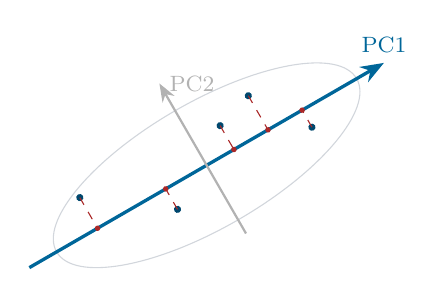
\begin{tikzpicture}[scale=1.0,>=Stealth]
  % tilted point cloud (rotated ellipse), PC1 along 30 deg
  \begin{scope}[rotate=30]
    \draw[rulec] (0,0) ellipse [x radius=2.2cm, y radius=0.8cm];
    % PC1 arrow along long axis
    \draw[->,tuwblue,very thick] (-2.6,0) -- (2.6,0) node[above,font=\footnotesize] {PC1};
    % PC2 orthogonal, discarded
    \draw[->,gray!60,thick] (0,-1.0) -- (0,1.2) node[right,font=\footnotesize] {PC2};
  \end{scope}
  % a few sample points (in rotated frame coords, drawn via scope)
  \begin{scope}[rotate=30]
    \foreach \px/\py in {-1.6/0.45, -0.6/-0.3, 0.4/0.35, 1.4/-0.25, 0.9/0.5} {
      \fill[tuwdark] (\px,\py) circle (1.3pt);
      % perpendicular onto PC1 (the x-axis of rotated frame)
      \draw[dashed,pitred,thin] (\px,\py) -- (\px,0);
      \fill[pitred] (\px,0) circle (1pt);
    }
  \end{scope}
\end{tikzpicture}
\end{center}
\sketchnote{Draw an elongated 2D point cloud. Draw an arrow through its long
axis (PC1). Drop a perpendicular from each point onto that line; the feet of
the perpendiculars are the 1D coordinates. PC2 is orthogonal and discarded.}
\end{algobox}

\begin{algobox}[Recursive subdivision -- mosaic / treemap sketch]
Both split a rectangle proportionally and recurse.
\begin{center}
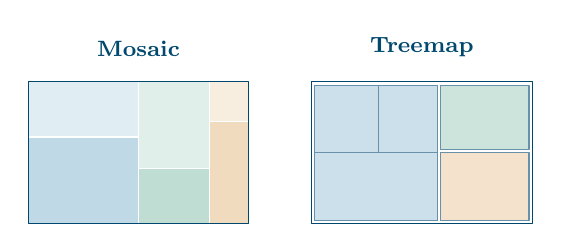
\begin{tikzpicture}[scale=1.0,line join=round]
  % --- Mosaic: width by A, then each column's height by B ---
  \begin{scope}
    \node[above,font=\footnotesize\bfseries,tuwdark] at (1.4,2.0) {Mosaic};
    % three columns of widths 1.4, 0.9, 0.5 (A proportions); total 2.8 wide, 1.8 tall
    % column 1
    \fill[tuwblue!25] (0,0) rectangle (1.4,1.1);
    \fill[tuwblue!12] (0,1.1) rectangle (1.4,1.8);
    % column 2
    \fill[keygreen!25] (1.4,0) rectangle (2.3,0.7);
    \fill[keygreen!12] (1.4,0.7) rectangle (2.3,1.8);
    % column 3
    \fill[examorange!25] (2.3,0) rectangle (2.8,1.3);
    \fill[examorange!12] (2.3,1.3) rectangle (2.8,1.8);
    % borders
    \draw[white,thin] (1.4,0)--(1.4,1.8) (2.3,0)--(2.3,1.8)
                      (0,1.1)--(1.4,1.1) (1.4,0.7)--(2.3,0.7) (2.3,1.3)--(2.8,1.3);
    \draw[tuwdark,thin] (0,0) rectangle (2.8,1.8);
  \end{scope}
  % --- Treemap: nested rectangles ---
  \begin{scope}[xshift=3.6cm]
    \node[above,font=\footnotesize\bfseries,tuwdark] at (1.4,2.0) {Treemap};
    \draw[tuwdark,thin] (0,0) rectangle (2.8,1.8);
    \fill[tuwblue!20] (0.04,0.04) rectangle (1.6,1.76);
    \fill[keygreen!20] (1.64,0.94) rectangle (2.76,1.76);
    \fill[examorange!20] (1.64,0.04) rectangle (2.76,0.9);
    % recurse inside first child
    \draw[tuwdark!60,thin] (0.04,0.04) rectangle (1.6,1.76);
    \draw[tuwdark!60,thin] (0.04,0.9) rectangle (0.85,1.76);
    \draw[tuwdark!60,thin] (0.04,0.04) rectangle (1.6,0.9);
    \draw[tuwdark!60,thin] (1.64,0.94) rectangle (2.76,1.76);
    \draw[tuwdark!60,thin] (1.64,0.04) rectangle (2.76,0.9);
  \end{scope}
\end{tikzpicture}
\end{center}
\sketchnote{Mosaic: split the full width by variable~A's proportions, then
split each resulting column's height by variable~B's conditional proportions;
tile area = joint frequency. Treemap: split the rectangle by the top-level
children's summed values, then recurse inside each child; leaf area = value.}
\end{algobox}

\begin{algobox}[Hexagon binning sketch]
\begin{center}
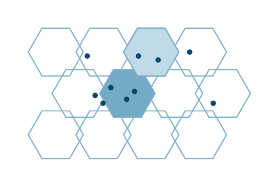
\begin{tikzpicture}[scale=1.0]
  % hexagon parameters: minimum size gives the diameter (point-to-point)
  \def\hs{0.7cm}     % hex minimum size
  \def\dx{0.606}     % horizontal spacing approx = 0.866*0.7
  \def\dy{0.525}     % vertical row offset = 0.75*0.7
  % grid of hexagons, offset rows; shade two by "count"
  \foreach \row in {0,1,2} {
    \foreach \col in {0,1,2,3} {
      \pgfmathsetmacro{\cx}{\col*0.866*0.7 + mod(\row,2)*0.433*0.7}
      \pgfmathsetmacro{\cy}{\row*0.525}
      % choose a couple of shaded ones
      \ifnum\row=1 \ifnum\col=1 \def\fc{tuwblue!55}\else\def\fc{none}\fi
      \else \ifnum\row=1 \def\fc{none}\else \def\fc{none}\fi \fi
      \node[regular polygon, regular polygon sides=6, draw=tuwblue!50, thin,
            minimum size=\hs, inner sep=0pt] at (\cx,\cy) {};
    }
  }
  % shade specific hexagons by count
  \node[regular polygon, regular polygon sides=6, draw=tuwblue!50, thin,
        fill=tuwblue!55, minimum size=\hs, inner sep=0pt]
        at ({1*0.866*0.7 + 0.433*0.7},{1*0.525}) {};
  \node[regular polygon, regular polygon sides=6, draw=tuwblue!50, thin,
        fill=tuwblue!25, minimum size=\hs, inner sep=0pt]
        at ({2*0.866*0.7},{2*0.525}) {};
  % scatter dots overlaid
  \foreach \px/\py in {0.5/0.5,0.7/0.6,0.9/0.45,1.0/0.55,0.6/0.4,
                       1.05/1.0,1.3/0.95,1.7/1.05,0.4/1.0,2.0/0.4} {
    \fill[tuwdark] (\px,\py) circle (1pt);
  }
\end{tikzpicture}
\end{center}
\sketchnote{Overlay a hexagonal grid on the scatterplot, count points per
hexagon, and fill each hexagon with a sequential colour by count. Replaces a
dense black blob with a readable density field.}
\end{algobox}

\begin{algobox}[KDE -- bandwidth sketch]
\begin{center}
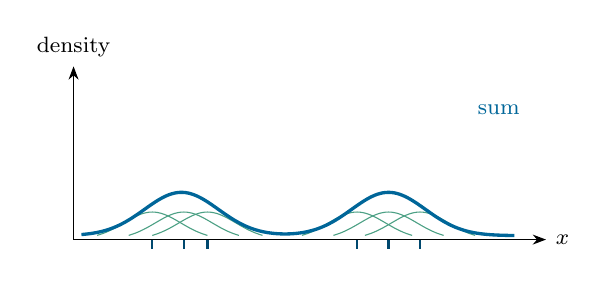
\begin{tikzpicture}[scale=1.0,>=Stealth]
  % axis
  \draw[->] (0,0) -- (6,0) node[right,font=\footnotesize] {$x$};
  \draw[->] (0,0) -- (0,2.2) node[above,font=\footnotesize] {density};
  % data points (ticks)
  \foreach \dx in {1.0,1.4,1.7,3.6,4.0,4.4} {
    \draw[tuwdark,thick] (\dx,0) -- (\dx,-0.12);
  }
  % small individual kernels (bumps) over each point
  \foreach \dx in {1.0,1.4,1.7,3.6,4.0,4.4} {
    \draw[keygreen!70,thin,smooth] plot[domain=\dx-0.7:\dx+0.7,samples=20]
      (\x, {0.35*exp(-((\x-\dx)*(\x-\dx))/(2*0.13))});
  }
  % bolder summed (good bandwidth) bimodal curve above
  \draw[tuwblue,very thick,smooth] plot[domain=0.1:5.6,samples=80]
    (\x, {0.55*exp(-((\x-1.37)*(\x-1.37))/(2*0.22))
          + 0.55*exp(-((\x-4.0)*(\x-4.0))/(2*0.22)) + 0.05});
  \node[tuwblue,font=\footnotesize] at (5.4,1.65) {sum};
\end{tikzpicture}
\end{center}
\sketchnote{Place a small bump (kernel) on each data point on the x-axis and
sum them into a smooth curve. Show three curves: tiny bandwidth (spiky,
overfit), good bandwidth (smooth bimodal), huge bandwidth (one flat hump,
oversmoothed).}
\end{algobox}

\begin{algobox}[Force-directed layout sketch]
\begin{center}
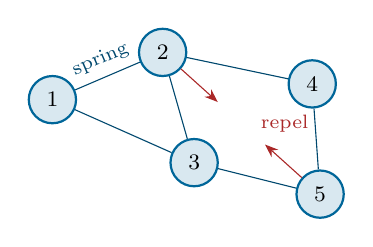
\begin{tikzpicture}[scale=1.0,>=Stealth,
    nd/.style={circle,draw=tuwblue,fill=tuwblue!15,thick,minimum size=6mm,inner sep=0pt,font=\footnotesize}]
  % five nodes
  \node[nd] (a) at (0,1.4) {1};
  \node[nd] (b) at (1.4,2.0) {2};
  \node[nd] (c) at (1.8,0.6) {3};
  \node[nd] (d) at (3.3,1.6) {4};
  \node[nd] (e) at (3.4,0.2) {5};
  % edges (one labelled spring)
  \draw[tuwdark] (a) -- node[above,font=\scriptsize,sloped] {spring} (b);
  \draw[tuwdark] (a) -- (c);
  \draw[tuwdark] (b) -- (c);
  \draw[tuwdark] (b) -- (d);
  \draw[tuwdark] (d) -- (e);
  \draw[tuwdark] (c) -- (e);
  % repulsion arrows (push apart) between two non-adjacent nodes
  \draw[->,pitred,thin] (b) -- ($(b)!0.35!(e)$);
  \draw[->,pitred,thin] (e) -- ($(e)!0.35!(b)$);
  \node[pitred,font=\scriptsize] at ($(b)!0.5!(e)+(0.55,0)$) {repel};
\end{tikzpicture}
\end{center}
\sketchnote{Nodes as charged particles repel each other; edges act as springs
pulling connected nodes together. Iterate until the energy settles. Draw a
small graph with well-separated nodes and short, roughly equal-length edges,
clusters visibly grouped.}
\end{algobox}

\begin{algobox}[Layered (Sugiyama) layout sketch]
\begin{center}
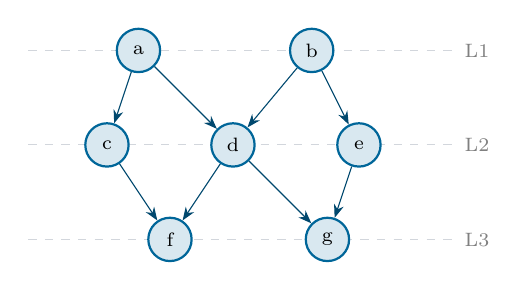
\begin{tikzpicture}[scale=1.0,>=Stealth,
    nd/.style={circle,draw=tuwblue,fill=tuwblue!15,thick,minimum size=5.5mm,inner sep=0pt,font=\scriptsize}]
  % three layer baselines (dashed)
  \foreach \y/\lbl in {2.4/L1, 1.2/L2, 0/L3} {
    \draw[dashed,rulec] (-0.4,\y) -- (5.0,\y);
    \node[gray,font=\scriptsize] at (5.3,\y) {\lbl};
  }
  % layer 1
  \node[nd] (a) at (1.0,2.4) {a};
  \node[nd] (b) at (3.2,2.4) {b};
  % layer 2
  \node[nd] (c) at (0.6,1.2) {c};
  \node[nd] (d) at (2.2,1.2) {d};
  \node[nd] (e) at (3.8,1.2) {e};
  % layer 3
  \node[nd] (f) at (1.4,0) {f};
  \node[nd] (g) at (3.4,0) {g};
  % downward edges, minimal crossings
  \draw[->,tuwdark] (a) -- (c);
  \draw[->,tuwdark] (a) -- (d);
  \draw[->,tuwdark] (b) -- (e);
  \draw[->,tuwdark] (b) -- (d);
  \draw[->,tuwdark] (c) -- (f);
  \draw[->,tuwdark] (d) -- (f);
  \draw[->,tuwdark] (d) -- (g);
  \draw[->,tuwdark] (e) -- (g);
\end{tikzpicture}
\end{center}
\sketchnote{Draw horizontal layers (rows). Place each node in a layer by its
topological rank; route all edges downward; reorder nodes within layers to
minimize crossings; insert dummy nodes for edges spanning multiple layers.}
\end{algobox}

\begin{algobox}[Counterfactual explanation sketch]
\begin{center}
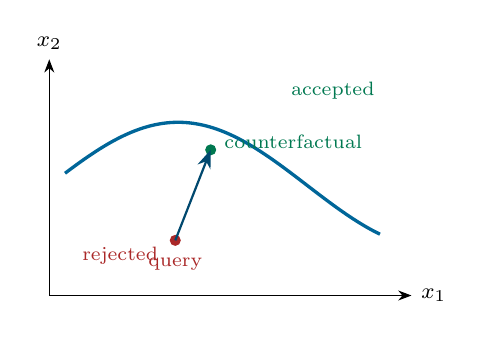
\begin{tikzpicture}[scale=1.0,>=Stealth]
  % feature space axes
  \draw[->] (0,0) -- (4.6,0) node[right,font=\footnotesize] {$x_1$};
  \draw[->] (0,0) -- (0,3.0) node[above,font=\footnotesize] {$x_2$};
  % curved decision boundary
  \draw[tuwblue,very thick,smooth] plot[domain=0.2:4.2,samples=60]
    (\x, {1.4 + 0.8*sin((\x*55)) });
  % region labels
  \node[pitred,font=\scriptsize] at (0.9,0.5) {rejected};
  \node[keygreen,font=\scriptsize] at (3.6,2.6) {accepted};
  % query point (rejected side)
  \fill[pitred] (1.6,0.7) circle (2pt);
  \node[pitred,font=\scriptsize,below] at (1.6,0.6) {query};
  % counterfactual: nearest point across boundary
  \fill[keygreen] (2.05,1.85) circle (2pt);
  \node[keygreen,font=\scriptsize,right] at (2.1,1.95) {counterfactual};
  % arrow from query to counterfactual
  \draw[->,tuwdark,thick] (1.6,0.7) -- (2.05,1.85);
\end{tikzpicture}
\end{center}
\sketchnote{Plot the decision boundary in feature space with the query point on
the ``rejected'' side. The counterfactual is the nearest point across the
boundary; draw the short arrow from query to that point -- the minimal,
sparse change that flips the outcome.}
\end{algobox}

\begin{algobox}[Partial dependence sketch]
\begin{center}
\begin{tikzpicture}[scale=1.0,>=Stealth]
  \draw[->] (0,0) -- (5.0,0) node[right,font=\footnotesize] {feature value};
  \draw[->] (0,0) -- (0,2.6) node[above,font=\footnotesize,align=center] {avg.\\prediction};
  % smooth response curve (rising then plateau)
  \draw[tuwblue,very thick,smooth] plot[domain=0.2:4.6,samples=60]
    (\x, {0.4 + 1.7/(1+exp(-2.2*(\x-2.2)))});
\end{tikzpicture}
\end{center}
\sketchnote{x-axis = one feature's value, y-axis = average model prediction.
For each grid value of the feature, set it for all rows, predict, and average.
Plot the resulting curve; its slope shows the feature's marginal effect.}
\end{algobox}

\section{List-Question Quick Reference}
\label{sec:lists}

Memorizable lists for the ``enumerate'' question type. Each item has a brief
gloss; in the exam, give the list and a one-line gloss per item.

% ---------------------------------------------------------------------
\subsection{Raw-data issues in data tables}
\begin{itemize}[leftmargin=1.4em]
  \item \term{Missing values} -- empty cells / NA; need imputation or removal.
  \item \term{Errors / outliers} -- typos, sensor faults, impossible values.
  \item \term{Duplicates} -- repeated records inflate counts.
  \item \term{Inconsistent units / formats} -- km vs.\ miles, date formats.
  \item \term{Inconsistent encoding} -- ``M''/``Male''/``1'' for same category.
  \item \term{Wrong data types} -- numbers stored as text, categorical as int.
  \item \term{Mixed granularity} -- rows at different aggregation levels.
  \item \term{Non-tidy structure} -- values in column names, multiple variables
        per column.
  \item \term{Skew / heavy tails / scale differences} -- may need log or
        normalization.
  \item \term{Imbalanced classes} -- distorts colour/area perception.
\end{itemize}

% ---------------------------------------------------------------------
\subsection{Factors affecting scalability}
\begin{itemize}[leftmargin=1.4em]
  \item \term{Number of data items} (rows) -- overplotting, slow rendering.
  \item \term{Number of dimensions / attributes} -- curse of dimensionality,
        too many axes/panels.
  \item \term{Number of categories} -- exhausts distinguishable colours/shapes.
  \item \term{Display resolution / screen pixels} -- pixel budget limits marks.
  \item \term{Human perception} -- limited channels, pre-attentive capacity
        (\term{perceptual scalability}).
  \item \term{Rendering / computation budget} -- frame rate, memory.
  \item \term{Interaction latency} -- query/response time
        (\term{interactive scalability}).
\end{itemize}

% ---------------------------------------------------------------------
\subsection{Sources of latency}
\begin{itemize}[leftmargin=1.4em]
  \item \term{Data transfer / network} -- moving data to the client.
  \item \term{Querying / aggregation} -- on-the-fly computation over big data.
  \item \term{Rendering} -- drawing many marks each frame.
  \item \term{Layout computation} -- e.g.\ force-directed iterations, DR.
  \item \term{Disk / IO} -- loading from storage.
  \item \term{Interaction round-trip} -- client$\leftrightarrow$server latency
        on brush/filter.
\end{itemize}

% ---------------------------------------------------------------------
\subsection{Aesthetic criteria for graph drawing}
\begin{itemize}[leftmargin=1.4em]
  \item \term{Minimize edge crossings.}
  \item \term{Uniform edge length} / minimize total edge length.
  \item \term{Even / symmetric node distribution}; display symmetries.
  \item \term{Angular resolution} -- large angles between edges at a node.
  \item \term{Minimize edge bends}; few orthogonal bends.
  \item \term{Avoid node/edge overlap.}
  \item \term{Cluster separation} -- communities visually grouped.
  \item \term{Consistent flow direction} (for directed/layered graphs).
  \item \term{Preserve the mental map} across changes (dynamic graphs).
\end{itemize}

% ---------------------------------------------------------------------
\subsection{Overplotting fixes that need no preprocessing}
\begin{itemize}[leftmargin=1.4em]
  \item \term{Transparency (alpha blending)} -- density shows through.
  \item \term{Smaller marks / thinner lines.}
  \item \term{Open glyphs} (outlines instead of filled).
  \item \term{Jitter} -- small random offset to separate coincident points.
  \item \term{Subsampling on the fly} (draw a random subset).
\end{itemize}
\begin{keybox}[Contrast]
Binning/hexbin, KDE, aggregation, and dimensionality reduction \emph{do} need
preprocessing -- do not list them as ``no-preprocessing'' fixes.
\end{keybox}

% ---------------------------------------------------------------------
\subsection{Model-agnostic AI interpretability methods}
\begin{itemize}[leftmargin=1.4em]
  \item \term{Partial dependence plots (PDP)} -- average marginal effect of a
        feature.
  \item \term{Individual conditional expectation (ICE)} -- per-instance PDP
        curves.
  \item \term{Permutation feature importance} -- accuracy drop when a feature
        is shuffled.
  \item \term{LIME} -- local surrogate from input perturbations.
  \item \term{SHAP} -- Shapley-value attribution of the prediction.
  \item \term{Counterfactual explanations} -- minimal change to flip outcome.
  \item \term{Local surrogate / global surrogate models.}
  \item \term{Accumulated local effects (ALE)} -- like PDP but robust to
        correlated features.
\end{itemize}

% ---------------------------------------------------------------------
\subsection{Techniques to visualize set-typed data}
\begin{itemize}[leftmargin=1.4em]
  \item \term{Venn / Euler diagrams} -- overlapping regions; poor beyond 3--4
        sets.
  \item \term{UpSet plots} -- matrix of intersections with bar charts; scales
        to many sets.
  \item \term{Set membership matrix} -- rows = elements, columns = sets.
  \item \term{Linear / radial set diagrams} (LineSets, Kelp diagrams, BubbleSets)
        -- overlays on a spatial layout.
  \item \term{Aggregate bar charts} of set / intersection sizes.
  \item \term{Parallel sets} -- flows between categorical set memberships.
\end{itemize}

% ---------------------------------------------------------------------
\subsection{Methods for validation of visual encoding and/or interaction design}
\begin{itemize}[leftmargin=1.4em]
  \item \term{Controlled experiment / user study} -- measure time \& accuracy.
  \item \term{Qualitative usability study} / think-aloud.
  \item \term{Expert review / heuristic evaluation.}
  \item \term{Case studies} with domain experts in the field.
  \item \term{Computational / algorithmic benchmarks} -- e.g.\ quality metrics
        (stress, class consistency, scagnostics).
  \item \term{Crowdsourced experiments} (e.g.\ MTurk) for many participants.
  \item \term{Analytical evaluation} against perceptual theory
        (expressiveness/effectiveness).
  \item \term{Log analysis} of real usage; A/B tests.
\end{itemize}

% ---------------------------------------------------------------------
\subsection{Typical dependent variables in user studies}
\begin{itemize}[leftmargin=1.4em]
  \item \term{Task completion time} (speed).
  \item \term{Accuracy / error rate} (correctness).
  \item \term{Confidence} ratings.
  \item \term{Subjective preference / satisfaction.}
  \item \term{Cognitive load} (e.g.\ NASA-TLX).
  \item \term{Insights found} / recall / memorability.
  \item \term{Eye-tracking measures} (fixations, scan path).
\end{itemize}

\section{Practice Questions with Model Answers}
\label{sec:practice}

Worked practice questions spanning all nine question types. Cover the question,
attempt your own answer, then check the model answer.

% =====================================================================
\begin{qbox}[Practice Q1 -- Literacy: confusion matrix (T/F)]
A 4-class action-recognition confusion matrix (rows = true class, columns =
predicted) has rows boxing, handwaving, jogging, running. Row sums are 100.
Diagonals: boxing 98, handwaving 95, jogging 60, running 80. Cell
(boxing,\,handwaving) $=0$; cell (jogging,\,running) $=30$.
Mark each True/False:
(1)~Boxing is never confused with handwaving.
(2)~Jogging is the hardest class to classify.
(3)~Jogging is most often confused with running.
(4)~Running is classified perfectly.

\medskip\noindent\textbf{Model answer.}
(1)~\term{True} -- cell is 0.
(2)~\term{True} -- smallest diagonal (60/100) = lowest recall.
(3)~\term{True} -- its largest off-diagonal cell (30) is the running column.
(4)~\term{False} -- diagonal 80, so 20\% misclassified. Always trace the exact
cell; remember rows are the true classes.
\end{qbox}

% =====================================================================
\begin{qbox}[Practice Q2 -- Algorithms: counterfactual (T/F)]
A loan model rejects an applicant. Mark which statements about \emph{counterfactual
explanations} are correct:
(1)~A good counterfactual changes as few features as possible.
(2)~There is exactly one counterfactual per instance.
(3)~Counterfactuals are model-agnostic and need no access to model internals.
(4)~The counterfactual should be plausible / actionable (e.g.\ not ``reduce age
by 10 years'').

\medskip\noindent\textbf{Model answer.}
Correct: \term{(1), (3), (4)}.
(2) is \term{False} -- many counterfactuals can exist (Rashomon effect); good
methods report close, sparse, plausible ones. (3) holds because counterfactuals
only query input$\to$output behaviour.
\end{qbox}

% =====================================================================
\begin{qbox}[Practice Q3 -- Strategy: 10M traffic-accident records]
A table has 10 million European traffic-accident records: (ID, longitude,
latitude, year). Design an interactive web visualization to explore the
distribution \emph{spatially and temporally}. How would you preprocess?

\medskip\noindent\textbf{Model answer (5-step template).}
\begin{enumerate}[leftmargin=1.4em]
  \item \term{Data type \& task.} Tall (10M rows) spatio-temporal point data;
        task = explore spatial and temporal distribution and their interaction.
  \item \term{Preprocessing / scalability.} The challenge is twofold:
        \emph{perceptual scalability} (10M points overplot any map) and
        \emph{interactive scalability} (raw queries are too slow). Solution:
        \term{spatial binning} (hexbin grid or aggregate to NUTS regions) and
        \term{temporal binning} (by year), with counts pre-aggregated into a
        \term{data cube} over (space-bin $\times$ year) for $O(1)$ slicing.
        Both spatial \emph{and} temporal binning are required.
  \item \term{Visual encoding.} Two views. Spatial: \term{choropleth} (regions)
        or \term{hexbin map}, marks = area cells, channel = colour by accident
        count using a \term{sequential} colour map. Temporal: \term{line chart}
        (or histogram), marks = line/bars, channel = position (x = year,
        y = count).
  \item \term{Interaction.} \term{Linked (coordinated) views}: \term{brush}
        a year range on the temporal chart to update the map, and \term{brush}
        regions on the map to filter the temporal chart (cross-filtering);
        plus zoom/pan and \term{details-on-demand} on hover.
  \item \term{Justify vs.\ alternatives.} Binned map beats raw scatter (no
        overplotting); data cube beats live aggregation (low latency);
        sequential beats rainbow (perceptually ordered). KDE on raw 10M points
        would be too slow / ineffective.
\end{enumerate}
\textit{Deductions to avoid: not naming the scalability challenge; no linked
views; only spatial or only temporal binning; missing marks/channels; rainbow
colour map; no mention of aggregation/data cube.}
\end{qbox}

% =====================================================================
\begin{qbox}[Practice Q4 -- Validation: user study for scatterplot class encodings]
Design a user study to evaluate the effectiveness of visual encodings of
classes/sets in \emph{static} scatterplots.

\medskip\noindent\textbf{Model answer.}
\term{Hypothesis (H1):} colour-coded classes yield faster and more accurate
class-separation judgments than shape-coded classes; \term{H2:} effectiveness
degrades as the number of classes grows.
\term{IV:} class encoding (colour / shape / colour+shape) and \#classes
(3 / 6 / 9).
\term{DV:} task completion time, accuracy/error rate, confidence, preference.
\term{Controlled:} number of points, degree of overlap, point size, display,
task wording, training.
\term{Confounds:} colour-vision deficiency (screen participants), learning/order
effects (counterbalance with a Latin square), fatigue.
\term{Design:} within-subjects, e.g.\ 24 participants; tasks = ``which class is
denser here?'' / ``find the outlier of class~X''; analyze with repeated-measures
ANOVA. Report effect sizes.
\end{qbox}

% =====================================================================
\begin{qbox}[Practice Q5 -- Critique: rainbow choropleth]
A regional-unemployment-rate map uses the rainbow (jet) colour scale. Critique
it and suggest a fix.

\medskip\noindent\textbf{Model answer.}
Problems: (i)~\term{rainbow is not perceptually ordered} -- viewers cannot rank
hues, so high vs.\ low is ambiguous; (ii)~\term{not perceptually uniform} --
equal data steps produce unequal perceived steps (false boundaries at
yellow/cyan); (iii)~\term{not colour-blind safe}; (iv)~mixes hue and lightness,
causing \term{channel interference}; (v)~rate (a magnitude) should use an
ordered channel. Fix: a \term{single-hue (or ColorBrewer) sequential} map
ordered by lightness; consider a \term{diverging} map if comparing against a
national-average reference. Also watch simultaneous contrast between adjacent
regions and the hidden choropleth bias toward large-area regions
(consider rate per capita / a cartogram).
\end{qbox}

% =====================================================================
\begin{qbox}[Practice Q6 -- Alternatives: parallel coordinates vs.\ SPLOM]
The same 8-dimensional dataset is shown as parallel coordinates (PCC) and as a
scatterplot matrix (SPLOM). Compare them.

\medskip\noindent\textbf{Model answer.}
\begin{itemize}[leftmargin=1.4em]
  \item \term{Dimension scalability:} PCC = one axis per dimension (handles many
        dims in one view); SPLOM = $O(d^2)$ panels (64 here), shrinking fast.
  \item \term{Task fit:} SPLOM shows \emph{all pairwise} correlations directly;
        PCC shows \emph{multivariate profiles, clusters, outliers} and
        correlation only between \emph{adjacent} axes.
  \item \term{Clutter:} PCC suffers heavy line overplotting on tall data;
        SPLOM suffers point overplotting per panel.
  \item \term{Ordering:} PCC depends strongly on \term{axis order}
        (non-adjacent relations hidden); SPLOM is order-insensitive.
  \item \term{Interaction:} PCC benefits from brushing + axis reordering; SPLOM
        from linked brushing across panels.
\end{itemize}
Recommendation: SPLOM for pairwise-correlation tasks at moderate $d$; PCC for
profile/cluster/outlier exploration at higher $d$ (with reorderable axes).
\end{qbox}

% =====================================================================
\begin{qbox}[Practice Q7 -- Transfer/sketch: array $\to$ histogram + boxplot]
Given the array $\{4, 5, 5, 6, 6, 6, 7, 8, 20\}$, sketch a histogram and a
boxplot.

\medskip\noindent\textbf{Model answer.}
Sorted $n=9$: median $=6$ (5th value); lower half $\{4,5,5,6\}\Rightarrow$
Q1$=5$; upper half $\{7,8,20\}\Rightarrow$ Q3$=8$; IQR$=3$; upper fence
$=8+1.5\cdot3=12.5\Rightarrow 20$ is an \term{outlier}; whisker max (non-outlier)
$=8$.
\begin{center}
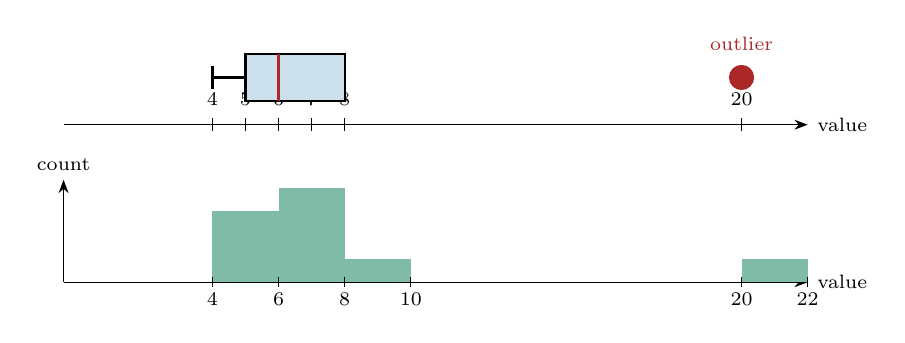
\begin{tikzpicture}[font=\scriptsize, x=0.42cm, y=1cm]
  % ---- boxplot (top) ----
  % axis 0..22 at y=2
  \draw[->,>=Stealth] (-0.5,2) -- (22,2) node[right] {value};
  \foreach \x in {4,5,6,7,8,20}
    \draw (\x,1.92) -- (\x,2.08) node[above=1pt] {\x};
  % whiskers from 4 to 5 and 8 to 8 (max non-outlier = 8)
  \draw[thick] (4,2.6) -- (5,2.6); % lower whisker line
  \draw[thick] (4,2.45) -- (4,2.75); % lower cap
  % box 5..8
  \draw[thick, fill=tuwblue!20] (5,2.3) rectangle (8,2.9);
  % median at 6
  \draw[thick, pitred] (6,2.3) -- (6,2.9);
  % upper whisker (box top = 8 = whisker max, draw small cap)
  \draw[thick] (8,2.45) -- (8,2.75);
  % outlier at 20
  \fill[pitred] (20,2.6) circle (0.16cm);
  \node[pitred, above=2pt] at (20,2.75) {outlier};
  % ---- histogram (bottom), bins width 2 ----
  % bins: [4,6):{4,5,5}=3 ; [6,8):{6,6,6,7}=4 ; [8,10):{8}=1 ; [20,22):{20}=1
  \draw[->,>=Stealth] (-0.5,0) -- (22,0) node[right] {value};
  \draw[->,>=Stealth] (-0.5,0) -- (-0.5,1.3) node[above] {count};
  \fill[keygreen!50] (4,0) rectangle (6,0.9);
  \fill[keygreen!50] (6,0) rectangle (8,1.2);
  \fill[keygreen!50] (8,0) rectangle (10,0.3);
  \fill[keygreen!50] (20,0) rectangle (22,0.3);
  \foreach \x in {4,6,8,10,20,22}
    \draw (\x,-0.06) -- (\x,0.06) node[below=2pt] {\x};
\end{tikzpicture}
\end{center}
\sketchnote{Boxplot: box from 5 to 8, median line at 6, lower whisker to 4,
upper whisker to 8, a separate dot at 20 marked as outlier. Histogram (bins of
width 2): tall bar around 5--6, smaller bars at 4 and 7--8, an isolated low bar
near 20 -- right-skewed.}
\end{qbox}

% =====================================================================
\begin{qbox}[Practice Q8 -- Mapping: scatterplot point $\to$ PCC polyline]
A scatterplot of (weight, mpg) highlights one outlier car: high weight, low mpg.
Mark the same car in a parallel-coordinates plot whose axes are, left to right,
mpg, weight, horsepower.

\medskip\noindent\textbf{Model answer.}
Recover its values: low on mpg, high on weight (horsepower unknown from the
scatter, but heavy cars are typically high). The car's \term{polyline} is the
one that is \term{low on the mpg axis and high on the weight axis} (and, for a
heavy car, high on horsepower). Trace the single line crossing those positions
and highlight it.
\begin{center}
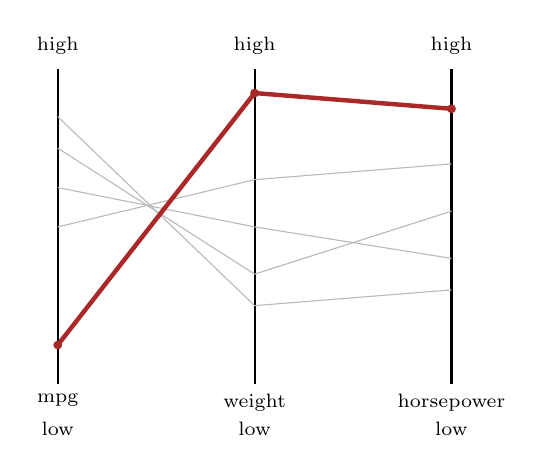
\begin{tikzpicture}[font=\scriptsize]
  % three vertical axes at x=0,2.5,5 ; y from 0 (low) to 4 (high)
  \foreach \x/\lab in {0/mpg, 2.5/weight, 5/horsepower}{
    \draw[thick] (\x,0) -- (\x,4);
    \node[below] at (\x,0) {\lab};
    \node[above=2pt] at (\x,4) {high};
    \node[below=10pt] at (\x,0) {low};
  }
  % faded background lines
  \draw[gray!55] (0,3.0) -- (2.5,1.4) -- (5,2.2);
  \draw[gray!55] (0,2.5) -- (2.5,2.0) -- (5,1.6);
  \draw[gray!55] (0,3.4) -- (2.5,1.0) -- (5,1.2);
  \draw[gray!55] (0,2.0) -- (2.5,2.6) -- (5,2.8);
  % highlighted outlier: low mpg, high weight, high horsepower
  \draw[ultra thick, pitred] (0,0.5) -- (2.5,3.7) -- (5,3.5);
  \fill[pitred] (0,0.5) circle (1.6pt) (2.5,3.7) circle (1.6pt) (5,3.5) circle (1.6pt);
\end{tikzpicture}
\end{center}
\sketchnote{Three vertical axes; one bold polyline starting low on mpg, rising
to the top of the weight axis, staying high on horsepower; other lines faded.}
\end{qbox}

% =====================================================================
\begin{qbox}[Practice Q9 -- MCQ: t-SNE properties]
Which statements about t-SNE are correct?
(a)~It is a linear projection.
(b)~Perplexity balances attention to local vs.\ global structure.
(c)~Distances between well-separated clusters are quantitatively meaningful.
(d)~Different random seeds can give different layouts.

\medskip\noindent\textbf{Model answer.} Correct: \term{(b), (d)}.
(a) is false (nonlinear); (c) is false (between-cluster distances and cluster
sizes are \emph{not} reliable). t-SNE is stochastic, so set a seed for
reproducibility.
\end{qbox}

% =====================================================================
\begin{qbox}[Practice Q10 -- MCQ: PCA vs.\ UMAP]
Pick the correct pairings.
(a)~PCA axes are interpretable directions of maximum variance.
(b)~UMAP is deterministic.
(c)~UMAP's \texttt{n\_neighbors} trades local detail for global structure.
(d)~PCA can capture nonlinear manifolds.

\medskip\noindent\textbf{Model answer.} Correct: \term{(a), (c)}.
(b) false -- UMAP is stochastic. (d) false -- PCA is linear; use t-SNE/UMAP/MDS
or kernel PCA for nonlinear structure.
\end{qbox}

% =====================================================================
\begin{qbox}[Practice Q11 -- MCQ: force-directed layout]
Which hold for force-directed graph layout?
(a)~It is deterministic regardless of initialization.
(b)~It models edges as springs and nodes as mutually repelling charges.
(c)~Naive computation is $O(n^2)$ per iteration; Barnes--Hut approximates it.
(d)~It guarantees the global minimum-energy layout.

\medskip\noindent\textbf{Model answer.} Correct: \term{(b), (c)}.
(a) false -- the result depends on the random initial placement. (d) false --
it can settle in a local minimum.
\end{qbox}

% =====================================================================
\begin{qbox}[Practice Q12 -- List: overplotting fixes with no preprocessing]
List simple solutions to overplotting that require \emph{no} data preprocessing.

\medskip\noindent\textbf{Model answer.}
\term{Transparency (alpha)}, \term{smaller marks}, \term{open glyphs},
\term{jitter}, \term{on-the-fly subsampling}. (Hexbin, KDE, aggregation, and
DR are effective but \emph{do} require preprocessing, so they do not count.)
\end{qbox}

% =====================================================================
\begin{qbox}[Practice Q13 -- Algorithms: sketch 1D PCA]
Sketch the 1D PCA projection of an elongated 2D cloud tilted at about
$30^{\circ}$.

\medskip\noindent\textbf{Model answer.}
\begin{center}
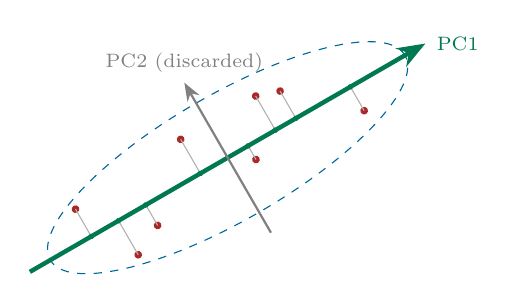
\begin{tikzpicture}[font=\scriptsize, rotate=30]
  % elongated cloud tilted 30 deg (whole picture rotated)
  \draw[tuwblue, dashed] (0,0) ellipse (2.6cm and 0.8cm);
  % PC1 arrow along long axis (x), PC2 short axis (y)
  \draw[->,>=Stealth, ultra thick, keygreen] (-2.9,0) -- (2.9,0) node[right] {PC1};
  \draw[->,>=Stealth, thick, gray] (0,-1.1) -- (0,1.1) node[above] {PC2 (discarded)};
  % data points and their perpendicular projections (feet) onto PC1
  \foreach \px/\py in {-2.0/0.4, -1.2/-0.3, -0.4/0.5, 0.3/-0.2, 1.0/0.4, 1.8/-0.35, -1.6/-0.5, 0.7/0.5}{
    \fill[pitred] (\px,\py) circle (1.4pt);
    \draw[gray!60, thin] (\px,\py) -- (\px,0);
    \fill[keygreen] (\px,0) circle (1.0pt);
  }
\end{tikzpicture}
\end{center}
\sketchnote{Draw the tilted elliptical cloud. Draw PC1 as an arrow along its
long axis (max variance). Project each point perpendicularly onto PC1; the feet
of those perpendiculars are the 1D coordinates. PC2 (orthogonal, short axis) is
discarded.}
PCA is linear and deterministic; PC1 captures the most variance.
\end{qbox}

% =====================================================================
\begin{qbox}[Practice Q14 -- List: model-agnostic interpretability methods]
Name model-agnostic methods to interpret an ML model.

\medskip\noindent\textbf{Model answer.}
\term{PDP} (average marginal effect), \term{ICE} (per-instance curves),
\term{permutation feature importance}, \term{LIME} (local surrogate),
\term{SHAP} (Shapley attribution), \term{counterfactual explanations},
\term{ALE plots}, and global \term{surrogate models}. All treat the model as a
black box, querying only inputs$\to$outputs.
\end{qbox}


\end{document}
